\documentclass[hess, manuscript]{copernicus}
%DIF LATEXDIFF DIFFERENCE FILE
%DIF DEL /home/adam/Downloads/climate_et/doc/paper/vpd_et_paper_hess.tex   Thu Feb 28 23:52:23 2019
%DIF ADD ./vpd_et_paper_hess.tex                                           Thu Feb 28 19:07:07 2019

\usepackage{makecell} \usepackage{multirow} %AM for tables
\usepackage{hyperref}
\usepackage[title]{appendix}
\usepackage{booktabs}
\usepackage{longtable}

\newcommand{\appropto}{\mathrel{\vcenter{
      \offinterlineskip\halign{\hfil$##$\cr
        \propto\cr\noalign{\kern2pt}\sim\cr\noalign{\kern-2pt}}}}}
%DIF PREAMBLE EXTENSION ADDED BY LATEXDIFF
%DIF UNDERLINE PREAMBLE %DIF PREAMBLE
\RequirePackage[normalem]{ulem} %DIF PREAMBLE
\RequirePackage{color}\definecolor{RED}{rgb}{1,0,0}\definecolor{BLUE}{rgb}{0,0,1} %DIF PREAMBLE
\providecommand{\DIFaddtex}[1]{{\protect\color{blue}\uwave{#1}}} %DIF PREAMBLE
\providecommand{\DIFdeltex}[1]{{\protect\color{red}\sout{#1}}}                      %DIF PREAMBLE
%DIF SAFE PREAMBLE %DIF PREAMBLE
\providecommand{\DIFaddbegin}{} %DIF PREAMBLE
\providecommand{\DIFaddend}{} %DIF PREAMBLE
\providecommand{\DIFdelbegin}{} %DIF PREAMBLE
\providecommand{\DIFdelend}{} %DIF PREAMBLE
%DIF FLOATSAFE PREAMBLE %DIF PREAMBLE
\providecommand{\DIFaddFL}[1]{\DIFadd{#1}} %DIF PREAMBLE
\providecommand{\DIFdelFL}[1]{\DIFdel{#1}} %DIF PREAMBLE
\providecommand{\DIFaddbeginFL}{} %DIF PREAMBLE
\providecommand{\DIFaddendFL}{} %DIF PREAMBLE
\providecommand{\DIFdelbeginFL}{} %DIF PREAMBLE
\providecommand{\DIFdelendFL}{} %DIF PREAMBLE
%DIF END PREAMBLE EXTENSION ADDED BY LATEXDIFF
%DIF PREAMBLE EXTENSION ADDED BY LATEXDIFF
%DIF HYPERREF PREAMBLE %DIF PREAMBLE
\providecommand{\DIFadd}[1]{\texorpdfstring{\DIFaddtex{#1}}{#1}} %DIF PREAMBLE
\providecommand{\DIFdel}[1]{\texorpdfstring{\DIFdeltex{#1}}{}} %DIF PREAMBLE
%DIF END PREAMBLE EXTENSION ADDED BY LATEXDIFF

\begin{document}

\title{When does vapor pressure deficit drive or reduce
  evapotranspiration?}
\Author[1]{Adam}{Massmann}
\Author[1]{Pierre}{Gentine}
\Author[1,2]{Changjie}{Lin}


\affil[1]{Department of Earth and Environmental Engineering,
  Columbia University, New York, NY 10027}
\affil[2]{State Key Laboratory of Hydroscience and Engineering, Department of Hydraulic
  Engineering, Tsinghua University, Beijing, CN 100084}

\runningtitle{When does VPD drive or reduce ET?}

\runningauthor{A. Massmann}

\correspondence{Adam Massmann (akm2203@columbia.edu)}


\firstpage{1}

\maketitle

\begin{abstract}
Increasing vapor pressure deficit (VPD) increases atmospheric demand
for water, and vapor pressure deficit is expected to rise with
increasing greenhouse gases. While increased evapotranspiration (ET)
in response to increased atmospheric demand seems intuitive, plants
are capable of reducing ET in response to increased VPD by closing
their stomata, in an effort to conserve water. Here we examine which
effect dominates response to increasing VPD: atmospheric demand and
increases in ET, or plant physiological response (stomata closure) and
decreases in ET. We use Penman-Monteith, combined with semi-empirical
optimal stomatal regulation theory and underlying water use
efficiency, to develop a theoretical framework for understanding how
ET responds to increases in VPD. \DIFdelbegin %DIFDELCMD <

%DIFDELCMD < %%%
\DIFdel{The theory suggests that for most }\DIFdelend \DIFaddbegin \DIFadd{The theoretical ET response to VPD
over a range of reasonable }\DIFaddend environmental conditions and plant
\DIFdelbegin \DIFdel{types, plant physiological response dominates and ET decreases with
increasing VPD . Plants that are evolved or bred to prioritize primary
production over water conservation (e.g.
crops) exhibit a higher
likelihood of atmospheric demand-driven response (ET increasing). However for forest, grass, savannah, and shrub plant types, ET more frequently decreases than increases with rising VPD. This work
serves as an example of }\DIFdelend \DIFaddbegin \DIFadd{characteristics varies from a strong decrease in ET in response to
increasing VPD (water conservative) to a strong increase in ET in
response to VPD (water intensive), highlighting the diversity of plant
water regulation strategies.
}

\DIFadd{The ET response varies due to: 1) climate, with tropical and temperate
climates more likely to exhibit a positive ET response to increasing
VPD than boreal and arctic climates; 2) photosynthesis strategy, with
C3 plants more likely to exhibit a positive ET response than C4
plants; and 3) due to plant type, with crops more likely to exhibit a
positive ET response, and shrubs and gymniosperm trees more likely to
exhibit a negative ET response. These results, derived from previous
literature connecting plant parameters to plant and climate
characteristics, highlight }\DIFaddend the utility of our simplified framework for
\DIFdelbegin \DIFdel{disentangling land-atmosphere feedbacks, including
the characterization of ET response in an atmospherically drier,
enriched CO$_2$ world.
}%DIFDELCMD <

%DIFDELCMD < %%%
\DIFdelend \DIFaddbegin \DIFadd{understanding complex land atmosphere systems in terms of idealized
scenarios in which evapotranspiration responds to VPD only. This
response is otherwise challenging to assess in an environment where
many processes co-evolve together.
}\DIFaddend \end{abstract}

\introduction
Vapor pressure deficit (VPD) is expected to rise over continents in
the future due to the combination of increased temperature and,
depending on region, decreased relative humidity
\citep{Byrne_2013}. Increases in VPD increase the atmospheric demand
for evapotranspirated water \citep{Penman_1948, Monteith_1965}, but
also \DIFdelbegin \DIFdel{stress plant stomata \mbox{%DIFAUXCMD
\citep{Leuning_1990, MEDLYN_2011}}%DIFAUXCMD
}\DIFdelend \DIFaddbegin \DIFadd{reduce stomatal conductance through stomatal closure
\mbox{%DIFAUXCMD
\citep{Rawson1977, Leuning_1990, Mott2007, Damour2010,
MEDLYN_2011}}%DIFAUXCMD
. Understanding the net evapotranspiration (ET) response
to these two opposing effects of changes in VPD is crucial for
assessing the impact of environmental VPD perturbations on the water
cycle}\DIFaddend .

The opposing effects of increased atmospheric demand and higher
stomatal \DIFdelbegin \DIFdel{stress }\DIFdelend \DIFaddbegin \DIFadd{closure }\DIFaddend lead to two possible perspectives for how \DIFdelbegin \DIFdel{evapotranspiration (ET ) }\DIFdelend \DIFaddbegin \DIFadd{ET }\DIFaddend responds
to shifts in VPD. The first, a hydrometeorological perspective, is
that higher VPD increases atmospheric demand for water from the land
surface, and this drives an increase in \DIFdelbegin \DIFdel{evapotranspiration (ET
). This perspective is particularly
relevant because potential evapotranspiration (PET), which is used in
many drought indices and hydrometeorological studies
\mbox{%DIFAUXCMD
\citep[e.g.,][]{Heim_2002, Scheff_2015}}%DIFAUXCMD
, typically only quantifies
changes in atmospheric demand and fails to account for ecosystem
response \mbox{%DIFAUXCMD
\citep{Swann_2016}}%DIFAUXCMD
. In reality}\DIFdelend \DIFaddbegin \DIFadd{ET
\mbox{%DIFAUXCMD
\citep{Penman_1948}}%DIFAUXCMD
. However}\DIFaddend , plants' stomata have evolved to
optimally regulate the exchange of water and carbon, and tend to
partially close in response to increased atmospheric dryness
\DIFdelbegin \DIFdel{\mbox{%DIFAUXCMD
\citep{Farquhar_1978, Ball_1987, Leuning_1990, MEDLYN_2011}}%DIFAUXCMD
}\DIFdelend \DIFaddbegin \DIFadd{\mbox{%DIFAUXCMD
\citep{Farquhar_1978, Ball_1987, Leuning_1990, Katul_2009,
MEDLYN_2011}}%DIFAUXCMD
}\DIFaddend . This leads to a plant physiology perspective, in which
an increase in VPD \DIFdelbegin \DIFdel{,
particularly in well-watered soil conditions, }\DIFdelend may actually correspond to a decrease in ET because
of stomatal closure \citep[e.g.][]{Rigden_2017}.  In other words, the
question ``When does VPD drive or reduce ET?'' can be related to
whether plant regulation or atmospheric demand dominates \DIFaddbegin \DIFadd{the }\DIFaddend ET
response.

The ET response to changes in VPD alters water partitioning between
the soil and atmosphere. If ecosystem plant response reduces ET with
atmospheric drying then soil moisture will be better conserved. This
represents a sensible evolutionary strategy to cope with aridity: save
water for periods when atmospheric demand for water is relatively low,
and atmospheric carbon can be accessed with a relatively smaller cost
in water loss. If instead stomata were fully passive \citep [similar
to soil pores, e.g. ][]{Or_2013}, increased atmospheric aridity would
strongly reduce soil moisture \citep{Berg_2017}. This could further
increase aridity as low soil moisture levels increases the Bowen
ratio, leading to increased temperature and atmospheric drying
\DIFdelbegin \DIFdel{\mbox{%DIFAUXCMD
\citep[][]{Bouchet_1963, Morton_1965, Brutsaert_1999, Ozdogan_2006,
  Salvucci_2013, Gentine_2016, Berg_2016}}%DIFAUXCMD
}\DIFdelend \DIFaddbegin \DIFadd{\mbox{%DIFAUXCMD
\citep[][]{Bouchet_1963, Morton_1965, Brutsaert_1999, Ozdogan_2006,
Salvucci_2013, Gentine_2016, Berg_2016, Zhou_2019}}%DIFAUXCMD
}\DIFaddend . Therefore, passive
regulation and a lack of soil moisture conservation does not seem to
be a sensible strategy for plants from an evolutionary
standpoint. \DIFdelbegin %DIFDELCMD <

%DIFDELCMD < %%%
\DIFdel{As a counterpoint, one may argue that increases in ET with increasing
VPD could increase the likelihood of precipitation
\mbox{%DIFAUXCMD
\citep[e.g.,][]{Findell_2011}}%DIFAUXCMD
. However, increases in ET do not always
guarantee an increased likelihood of precipitation, which depending on
environmental conditions could cause a decrease in the likelihood of
precipitation \mbox{%DIFAUXCMD
\citep[][]{Gentine_2013}}%DIFAUXCMD
. Furthermore, any increases in
precipitation are likely to be non-local, such that plants
giving up
water to the atmosphere are not guaranteed to reap the benefits of
water returned from the atmosphere to the soil. Using this subjective
logic, from an ecosystem evolutionary perspective, water stored in
soil seems to be worth much more than the chance of water returned as
precipitation}\DIFdelend \DIFaddbegin \DIFadd{This simplified logic explains generally why plants
evolved to respond to VPD, but also excludes many details and special
cases (e.g. plant to plant interaction and highly specialized
photosynthesis strategies like Crassulacean acid metabolism
photosynthesis)}\DIFaddend .

We can use intuition about plant water conservation strategy to
hypothesize about ET response to changes in VPD. Plants and ecosystems
that evolved to conserve water, such as arid shrubs\DIFdelbegin \DIFdel{or savannah}\DIFdelend , should be more
likely to reduce ET with increasing VPD, and plants that have evolved
or have been engineered to \DIFdelbegin \DIFdel{care little about water
}\DIFdelend \DIFaddbegin \DIFadd{prioritize carbon gain over water
conservation}\DIFaddend , such as crops, will be more likely to increase ET with
increasing VPD. Atmospheric conditions must matter as well. At the
ecosystem scale, there are limits to plant water conservation
strategies. As atmospheric demand for water (VPD) increases,
ecosystems \DIFdelbegin \DIFdel{should }\DIFdelend \DIFaddbegin \DIFadd{may }\DIFaddend begin to reach their water conservation limits and
might not be able to entirely limit ET flux to the atmosphere. At this
stage any further increase in VPD will most likely drive a (limited)
increase in ET, because the increase in atmospheric demand for water
overwhelms the limited plant response to conserve water.

The objective of the present manuscript is to use reasonable
approximations \DIFaddbegin \DIFadd{established in prior research }\DIFaddend as a tool to develop \DIFdelbegin \DIFdel{intuition for plant response }\DIFdelend \DIFaddbegin \DIFadd{a
framework for understanding plant responses }\DIFaddend to atmospheric drying and
\DIFdelbegin \DIFdel{evaluate }\DIFdelend \DIFaddbegin \DIFadd{the }\DIFaddend the VPD dependence of ET \DIFdelbegin \DIFdel{. This
intuition }\DIFdelend \DIFaddbegin \DIFadd{while keeping other variables fixed. This
framework }\DIFaddend will aid interpretation of observations, full complexity
models, and facilitate the disentanglement of complex land-atmosphere
feedbacks. In \DIFaddbegin \DIFadd{particular, our approach has applications for
understanding climate change impacts, given expected increases in VPD
with rising temperature.  In }\DIFaddend the past, similar \DIFaddbegin \DIFadd{simplified }\DIFaddend approaches
were used to understand interactions between stomatal conductance,
evapotranspiration and the environment \DIFdelbegin \DIFdel{\mbox{%DIFAUXCMD
\citep[e.g.,][]{Jarvis_1986, Mcnaughton_1991}}%DIFAUXCMD
. However , at
the time researchers ' understanding of the form of VPD's effect on
plant physiology was limited, so they could not
explore }\DIFdelend \DIFaddbegin \DIFadd{\mbox{%DIFAUXCMD
\citep[e.g.,][]{Jarvis_1984,
Jarvis_1986, Mcnaughton_1991}}%DIFAUXCMD
. However these researchers did not
explore explicitly }\DIFaddend the sensitivity of ET to VPD, including VPD's
effect on stomatal conductance and plant function.

\DIFdelbegin \DIFdel{Recent results have drastically improved }\DIFdelend \DIFaddbegin \DIFadd{Approaching the problem of ET response to VPD is aided by recent
results drastically improving }\DIFaddend our understanding of VPD's impact on
physiology, especially at the leaf level. \citet{MEDLYN_2011}
developed a model for leaf-scale stomatal conductance ($g_s$),
including VPD response, by combining an optimal photosynthesis theory
\DIFdelbegin \DIFdel{\mbox{%DIFAUXCMD
\citep{Cowan_1977} }%DIFAUXCMD
}\DIFdelend \DIFaddbegin \DIFadd{\mbox{%DIFAUXCMD
\citep{Cowan_1977, Katul_2009, Katul_2010} }%DIFAUXCMD
}\DIFaddend with an empirical approach,
and extended use of this model to the ecosystem scale in
\citet{Medlyn_2017}. Additionally, \citet{Zhou_2014} demonstrated that
a quantity underlying water use efficiency $\left(uWUE = \frac{GPP\;
\sqrt{VPD}}{ET}\right)$ properly captures a constant relationship
between GPP, ET, and VPD over a diurnal cycle at the ecosystem
scale. uWUE is also \DIFdelbegin \DIFdel{remarkably }\DIFdelend \DIFaddbegin \DIFadd{relatively }\DIFaddend well conserved in the growing season
across space and time, within a \DIFdelbegin \DIFdel{PFT
}\DIFdelend \DIFaddbegin \DIFadd{plant functional type (PFT)
}\DIFaddend \citep{Zhou_2015}.  While stomatal conductance parameterizations and
uWUE greatly simplify complex plant physiological processes, they
 still capture \DIFdelbegin \DIFdel{leading order }\DIFdelend ecosystem behavior for vegetated surfaces
\citep{Medlyn_2017, Zhou_2014}, and are \DIFdelbegin \DIFdel{novel }\DIFdelend \DIFaddbegin \DIFadd{useful }\DIFaddend tools to transparently
develop intuition for the behavior of complex \DIFdelbegin \DIFdel{, multiscale
ecohydrologic }\DIFdelend \DIFaddbegin \DIFadd{land-atmosphere }\DIFaddend systems.

In this manuscript, we leverage uWUE and recent developments in
stomatal conductance parameterizations \citep{MEDLYN_2011} \DIFaddbegin \DIFadd{with a
Penman-Monteith framework
}(\DIFadd{hereafter PM, }{\DIFadd{Penman1948,
Monteith1965}}) \DIFaddend to derive the theoretical one-way response of ET to VPD
with other environmental variables properly controlled for, i.e. we
develop a framework for evaluating the partial derivative of ET with
respect to VPD. \DIFdelbegin \DIFdel{For the first time, }\DIFdelend \DIFaddbegin \DIFadd{It is useful to disconnect the impact of VPD from
other variables as VPD is known to increase dramatically with future
climate and limit ET more than soil moisture \mbox{%DIFAUXCMD
\citep{Novick_2016}}%DIFAUXCMD
, but
disentangling VPD effects from soil moisture effects has been
difficult in previous research, given their co-variability
\mbox{%DIFAUXCMD
\citep[][]{Lin_2018, Zhou_2019}}%DIFAUXCMD
.  We are
able to disentangle the effect of VPD on ET because }\DIFaddend we explicitly
include VPD's full effect on stomatal conductance, including its
\DIFdelbegin \DIFdel{leading order }\DIFdelend impact on photosynthesis. \DIFdelbegin \DIFdel{Our theory is
validated and tested at multiple eddy-covariance stations spanning
various climates and plant functional types.
}%DIFDELCMD <

%DIFDELCMD < %%%
\section{\DIFdel{Materials and Methods}}
%DIFAUXCMD
\addtocounter{section}{-1}%DIFAUXCMD
\subsection{\DIFdel{Data}}
%DIFAUXCMD
\addtocounter{subsection}{-1}%DIFAUXCMD
%DIFDELCMD < %DIFDELCMD < \label{data}%%%
%DIFDELCMD < %%%
\DIFdel{We use both meteorological and eddy-covariance data from the FLUXNET2015
database (data available at }%DIFDELCMD < \sloppy
%DIFDELCMD < \url{https://fluxnet.fluxdata.org/data/fluxnet2015-dataset/} \sloppy%%%
\DIFdel{)
,
including all Tier 1 sites with at least four years of data and
observations of the variables described in the
methods section (Sect.
\ref{methods}). Sixty-six sites met these requirements, and were grouped
into nine plant functional types (PFT) according to the International
Geosphere-Biosphere Programme vegetation classification scheme
\mbox{%DIFAUXCMD
\citep{Loveland_1999}}%DIFAUXCMD
: cropland (CRO), grass (GRA), deciduous broadleaf
forest (DBF), evergreen broadleaf forest (EBF), evergreen needleleaf
forest (ENF), mixed forest (MF), closed shrub (CSH), savannah (SAV), and
woody savannah (WSA) (site locations and citations are in Fig.
\ref{map_fig} and Appendix \ref{flux_sites}, respectively). }%DIFDELCMD <

%DIFDELCMD < \begin{figure}[h]
%DIFDELCMD <   \centering 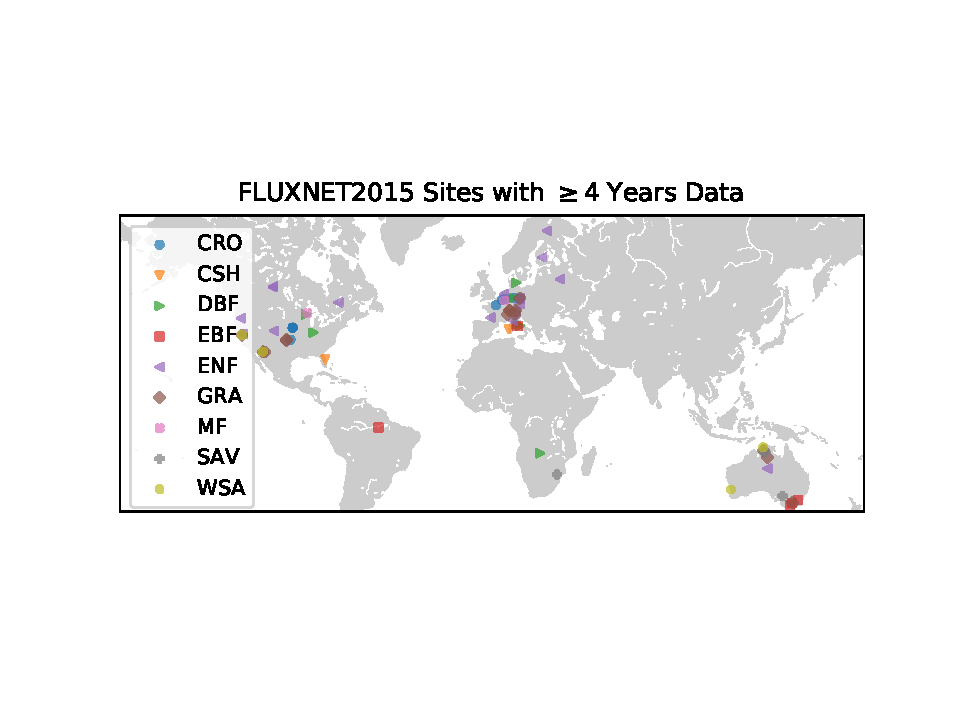
\includegraphics[trim={0 3cm 0 3cm}, clip]{./map.pdf}
%DIFDELCMD <   %%%
%DIFDELCMD < \caption{%
{%DIFAUXCMD
\DIFdelFL{Plant functional type and location of FLUXNET2015 sites
    used in this analysis.}}
  %DIFAUXCMD
%DIFDELCMD < \label{map_fig}
%DIFDELCMD < \end{figure}
%DIFDELCMD <

%DIFDELCMD < %%%
\DIFdel{The purpose of this study is to examine ecosystem response to
atmospheric drying, }\DIFdelend \DIFaddbegin \DIFadd{The use of an energy balance framework (PM)
allows us to include in our analysis the effects of the energy cost of
evaporating water from a surface, which is an important factor in the
natural environment, compared to prescribed in situ environmental
conditions. This is relevant because previous research }\DIFaddend focusing on the
\DIFdelbegin \DIFdel{growing season. To accomplish
this, }\DIFdelend \DIFaddbegin \DIFadd{leaf scale \mbox{%DIFAUXCMD
\citep{Rawson1977, Turner1984, Oren1999, Damour2010,
Mott2013} }%DIFAUXCMD
does not consistently or analogously include the energetic
constraints on evapotranspiration under which ecosystems operate. The
leaf-scale results agree that stomatal conductance decreases in
response to VPD \mbox{%DIFAUXCMD
\citep{Oren1999, Damour2010}}%DIFAUXCMD
, which we expect to be
true for an ecosystem as well. However leaf scale results also
indicate that transpiration usually increases with increasing VPD in a
concave downward shape \mbox{%DIFAUXCMD
\citep[e.g.,][]{Rawson1977, Turner1984,
Mott2013}}%DIFAUXCMD
, which may not be true for ET at the ecosystem scale once
energetic constraints on ET are included in the analysis.  Our
approach allows us to estimate the expected ET response to VPD at the
ecosystem scale, including the effects of surface energy balance
constraints, and assess how ecosystem ET response to VPD deviates from
previous leaf scale analyses.
}

\DIFadd{This manuscript presents the range of possible ecosystem-scale ET
responses to VPD, given parameters previously established in peer
reviewed literature. Additionally, }\DIFaddend we \DIFdelbegin \DIFdel{filter and quality control the data using a similar procedure
as \mbox{%DIFAUXCMD
\cite{Zhou_2015}}%DIFAUXCMD
:
}%DIFDELCMD < \begin{itemize}
 \begin{itemize} %DIFAUXCMD
%DIFDELCMD < \item %%%
\item%DIFAUXCMD
\DIFdel{Only measured or highest (``good'') quality gapfilled data,
  according to quality control flags, are used. }%DIFDELCMD < \item %%%
\item%DIFAUXCMD
\DIFdel{To isolate the growing season, we only use days in which the
  average Gross Primary Productivity (GPP) exceeds 10\% of the
  observed 95th percentile of GPP for a given site. GPP is calculated
  using the nighttime respiration partitioning method.  }%DIFDELCMD < \item %%%
\item%DIFAUXCMD
\DIFdel{We remove days with rain and the day following to avoid issues
  with rain interception and sensor saturation at high relative
  humidity (\mbox{%DIFAUXCMD
\cite{Medlyn_2017}}%DIFAUXCMD
).
}
 \end{itemize} %DIFAUXCMD
%DIFDELCMD < \end{itemize}
%DIFDELCMD < %%%
\DIFdel{Additionally, as in \mbox{%DIFAUXCMD
\citet{Lin_2018}}%DIFAUXCMD
, we restrict data to the daytime, which is identified when downwelling shortwave radiation is greater
than 50 W m$^{-2}$ and sensible heat flux is greater than 5 W
m$^{-2}$.
To reduce the chance of sensor saturation at high relative
humidity, we remove all time steps for which VPDis less than .01 kPa, and to reduce errors at low windspeeds we remove all periods with wind
magnitudes less than 0.5 m s$^{-1}$. Timesteps with negative observed
GPP or ET are also removed, and we aggregate half hourly data to
hourly averages to reduce noise \mbox{%DIFAUXCMD
\citep{Lin_2018}}%DIFAUXCMD
. After these quality
control procedures,
400, 983 upscaled hourly observations remain}\DIFdelend \DIFaddbegin \DIFadd{explore the sensitivity of the
ET-VPD relationship to stomatal model and framework choice,
highlighting the importance of: 1) future research on stomatal
conductance and ecosystem scale modeling, and 2) thoughtful selection
of photosynthesis and stomatal conductance models in more
sophisticated land surface and earth system models}\DIFaddend .


\DIFdelbegin \subsection{\DIFdel{Methods}}
%DIFAUXCMD
\addtocounter{subsection}{-1}%DIFAUXCMD
\DIFdelend \DIFaddbegin \section{\DIFadd{Methods}}
\DIFaddend \label{methods}
The Penman-Monteith equation \citep [hereafter PM,][]{Penman_1948,
  Monteith_1965} estimates ET as a function of observable atmospheric
variables and surface conductances:
% \begin{linenomath*}
  \begin{equation}
    \label{orig_pen}
    ET = \frac{\Delta R_{net} + g_a \rho_a c_p VPD}{\Delta + \gamma(1 + \frac{g_a}{g_s})},
  \end{equation}
% \end{linenomath*}
  where $\Delta$ is the change in saturation vapor pressure with
  temperature, given by Clausius-Clapeyron
  ($\frac{d \; e_s}{d \; T}$), $R_{net}$ is the net radiation minus
  ground heat flux, $g_a$ is aerodynamic conductance, $\rho_a$ is air
  density, $c_p$ is specific heat of air at constant pressure,
  $\gamma$ is the psychometric constant, and $g_s$ is the stomatal
  conductance (Table \ref{definitions}). \DIFaddbegin \DIFadd{The issue with PM is that
  $g_s$ is a function of carbon uptake, which is has a strong
  functionally relation to ET through stomatal function. Therefore,
  when PM is formulated in terms of $g_s$, it is an implicit function
  of ET itself rather than an explicit function of ET. Here we will
  derive a new form of PM in which ET is an explicit function of plant
  parameters and environmental conditions, and use it to assess the
  ecosystem scale response to VPD (by taking a partial derivative).
}\DIFaddend

\begin{table}
  \caption{Definition of symbols and variables, with citation for how
    values are calculated, if applicable.}
  \label{definitions}
  \centering \footnotesize
  \begin{tabular}{l c c c}
    \hline
    Variable & Description & Units & Citation \\
    \hline
    $e_s$  & saturation vapor pressure & Pa  & - \\
    $T$  & temperature  & K & - \\
    $P$  & pressure & Pa  & - \\
    $\Delta$  & $\frac{\partial e_s}{\partial T}$ & Pa K$^{-1}$ & - \\
    $R_{net}$  & net radiation at land surface minus ground heat flux & W m$^{-2}$   & - \\
    $g_a$  & aerodynamic conductance & m s$^{-1}$  & \citet{Shuttleworth_2012} \\
    $\rho_a$  & air density & kg m$^{-3}$  & - \\
    $c_p$  & specific heat capacity of air at constant pressure & J K$^{-1}$ kg$^{-1}$ & - \\
    $VPD$  & vapor pressure deficit & Pa  & - \\
    $\gamma$  & psychometric constant & Pa K$^{-1}$   & - \\
    \DIFdelbeginFL \DIFdelFL{$g_{s-leaf}$  }%DIFDELCMD < & %%%
\DIFdelFL{leaf-scale stomatal conductance }%DIFDELCMD < & %%%
\DIFdelFL{m s$^{-1}$  }%DIFDELCMD < & %%%
\DIFdelFL{\mbox{%DIFAUXCMD
\citet{MEDLYN_2011} }%DIFAUXCMD
}%DIFDELCMD < \\
%DIFDELCMD <     %%%
\DIFdelendFL $g_{s}$  &  stomatal conductance & m s$^{-1}$
                                   & \citet{Medlyn_2017} \\
    \DIFdelbeginFL \DIFdelFL{$g_{1-leaf}$  }%DIFDELCMD < & %%%
\DIFdelFL{leaf-scale slope parameter }%DIFDELCMD < & %%%
\DIFdelFL{Pa$^{0.5}$
                                   }%DIFDELCMD < & %%%
\DIFdelFL{\mbox{%DIFAUXCMD
\citet{MEDLYN_2011} }%DIFAUXCMD
}%DIFDELCMD < \\
%DIFDELCMD <     %%%
\DIFdelendFL $g_{1}$  & ecosystem-scale slope parameter & Pa$^{0.5}$ & \citet{Medlyn_2017} \\
    $R$ & universal gas constant & J mol$^{-1}$ K$^{-1}$ & - \\
    $R_{air}$ & gas constant of air & J  K$^{-1}$ kg$^{-1}$ & - \\
    $\sigma$ & uncertainty parameter & -& - \\
    $c_a$ & CO$_2$ concentration & $\mu$ mol CO$_2$ mol$^{-1}$ air& - \\
    \DIFdelbeginFL \DIFdelFL{$\lambda$ }\DIFdelendFL \DIFaddbeginFL \DIFaddFL{$\lambda = \frac{\partial \; transpiration}{\partial\; CO_2\; assimilation}$ }\DIFaddendFL & marginal water cost of leaf carbon & mol H$_2$O mol$^{-1}$ CO$_2$ & - \\
    $\Gamma$ & CO$_2$ compensation point & - & - \\
    $\Gamma^*$ & CO$_2$ compensation point without dark respiration &
                                                                      - & - \\
    \DIFaddbeginFL \DIFaddFL{GPP }& \DIFaddFL{gross primary production }& \DIFaddFL{$\mu$-mol C s$^{-1}$ m$^{-2}$ }& \DIFaddFL{-
    }\\
    \DIFaddFL{ET }& \DIFaddFL{evapotranspiration }& \DIFaddFL{W m$^{-2}$ }& \DIFaddFL{- }\\
   \DIFaddFL{uWUE }& \DIFaddFL{underlying water use efficiency }& \DIFaddFL{$\mu$-mol C Pa$^{0.5}$
                                            J$^{-1}$ ET  }&
                                                           \DIFaddFL{\mbox{%DIFAUXCMD
\citet{Zhou_2015} }%DIFAUXCMD
}\\
    \DIFaddendFL \hline
  \end{tabular}
\end{table}


\citet{MEDLYN_2011} developed a model for stomatal conductance ($g_s$)
by combining an optimal photosynthesis theory \citep{Cowan_1977} with
an empirical approach, which describes the dependence of $g_s$ to
VPD. \DIFdelbegin \DIFdel{This resulted in the following model for
leaf-scale stomatal conductance}\DIFdelend \DIFaddbegin \DIFadd{They also extended this model to the ecosystem scale
\mbox{%DIFAUXCMD
\citep{Medlyn_2017}}%DIFAUXCMD
}\DIFaddend :

% \begin{linenomath*}
  \begin{equation}
    g\DIFdelbegin \DIFdel{_{s-leaf} }\DIFdelend \DIFaddbegin \DIFadd{_s }\DIFaddend = \DIFdelbegin \DIFdel{g_0 + }\DIFdelend \DIFaddbegin \DIFadd{\frac{R \,T}{P} \; }\DIFaddend 1.6 \left(1 + \DIFdelbegin \DIFdel{\frac{g_{1-leaf}}{\sqrt{VPD}}}\DIFdelend \DIFaddbegin \DIFadd{\frac{g_1}{\sqrt{VPD}}}\DIFaddend \right) \DIFdelbegin \DIFdel{\frac{A}{c_a}}\DIFdelend \DIFaddbegin \DIFadd{\frac{GPP}{c_a}}\DIFaddend ,
    \DIFdelbegin %DIFDELCMD < \label{leaf_medlyn}
%DIFDELCMD <   %%%
\DIFdelend \DIFaddbegin \label{medlyn}
  \DIFaddend \end{equation}
% \end{linenomath*}
\DIFdelbegin \DIFdel{where $g_{1-leaf}$ is a leaf-scale }\DIFdelend \DIFaddbegin

  \DIFadd{where $g_{1}$ is a VPD }\DIFaddend ``slope'' parameter, \DIFdelbegin \DIFdel{A is the net
CO$_2$ assimilation rate}\DIFdelend \DIFaddbegin \DIFadd{GPP is the ecosystem
  scale gross primary production}\DIFaddend , and $c_a$ is the atmospheric CO$_2$
  concentration at the \DIFdelbegin \DIFdel{leaf surface}\DIFdelend \DIFaddbegin \DIFadd{canopy}\DIFaddend . \cite{MEDLYN_2011} relate the slope
  parameter (\DIFdelbegin \DIFdel{$g_{1-leaf}$}\DIFdelend \DIFaddbegin \DIFadd{$g_{1}$}\DIFaddend ) to physical parameters as:
% \begin{linenomath*}
\DIFdelbegin %DIFDELCMD < %DIFDELCMD < \label{slope}%%%
%DIFDELCMD <   %%%
\DIFdelend \DIFaddbegin

  \DIFaddend \begin{equation}
    g\DIFdelbegin \DIFdel{_{1-leaf} = }\DIFdelend \DIFaddbegin \DIFadd{_{1}  \propto }\DIFaddend \sqrt{\frac{3 \, \Gamma^* \,
        \lambda}{1.6}},\footnote{Note this expression has units of of
      (mmol mol$^{-1}$)$^{1/2}$, but this can be converted to
      Pa$^{1/2}$ using the ideal gas law.}
    \DIFaddbegin \label{slope}
  \DIFaddend \end{equation}
% \end{linenomath*}

where $\Gamma^*$ is the CO$_2$ compensation point for photosynthesis
(without dark respiration), and $\lambda$ is the marginal water cost
of leaf carbon
(\DIFdelbegin \DIFdel{$\frac{\partial \; \text{transpiration}}{\partial \; A}$)
}\DIFdelend \DIFaddbegin \DIFadd{$\frac{\partial \; \text{transpiration}}{\partial \; CO_2 assimilation}$)
\mbox{%DIFAUXCMD
\citep{Farquhar_1980, Katul_2009}}%DIFAUXCMD
}\DIFaddend . So,
\DIFdelbegin \DIFdel{$g_{1-leaf}$ }\DIFdelend \DIFaddbegin \DIFadd{$g_{1}$ }\DIFaddend is a leaf-scale term reflecting the trade-off of water for
carbon uptake. The higher \DIFdelbegin \DIFdel{$g_{1-leaf}$}\DIFdelend \DIFaddbegin \DIFadd{$g_{1}$}\DIFaddend , the more open the stomata and
the more they release water in exchange for carbon.


\DIFdelbegin \DIFdel{The Medlyn model for stomatal conductance has been shown to behave
very well across PFTs \mbox{%DIFAUXCMD
\citep[][]{Lin_2015}}%DIFAUXCMD
, and has been successfully
adopted to ecosystem scale analysis in \mbox{%DIFAUXCMD
\citet{Medlyn_2017}}%DIFAUXCMD
. In units
of m s$^{-1}$, the ecosystem scale stomatal conductance is:
}%DIFDELCMD <

%DIFDELCMD < %%%
%DIF <  \begin{linenomath*}
  \begin{displaymath}
    \DIFdel{g_s = \frac{R \,T}{P} \; 1.6 \left(1 + \frac{g_1}{\sqrt{VPD}}\right) \frac{GPP}{c_a},
    %DIFDELCMD < \label{medlyn}%%%
  }\end{displaymath}
%DIFAUXCMD
%DIF <  \end{linenomath*}
%DIFDELCMD <

%DIFDELCMD < %%%
\DIFdel{where GPP is the ecosystem scale gross primary production, and $g_1$
is an ecosystem scale analogue to $g_{1-leaf}$. We solve for $g_1$
following \mbox{%DIFAUXCMD
\citet{Medlyn_2017} }%DIFAUXCMD
(Eq. (5)), and take the median $g_1$
value to be representative of each PFT (Table \ref{pft}) instead of the mean to avoid extra weighting of rare outliers.
}%DIFDELCMD <

%DIFDELCMD < \begin{table}
%DIFDELCMD <   %%%
%DIFDELCMD < \caption{%
{%DIFAUXCMD
\DIFdelFL{Plant functional types, their abbreviation, calculated
    Medlyn coefficient, and calculated uWUE. uWUE from
    \mbox{%DIFAUXCMD
\citet{Zhou_2015}}%DIFAUXCMD
, including the observed standard deviation, is
    shown for comparison. Note that uWUE from \mbox{%DIFAUXCMD
\citet{Zhou_2015} }%DIFAUXCMD
is
    calculated from a different set of sites, and that units are
    converted such that the quantities work with Equations 1-8 and the
    variables defined Table \ref{definitions}.}}
  %DIFAUXCMD
%DIFDELCMD < \small
%DIFDELCMD <   %DIFDELCMD < \label{pft}%%%
%DIFDELCMD <   \centering
%DIFDELCMD <   \begin{tabular}{l c c @{\qquad} c c}
%DIFDELCMD <     \hline
%DIFDELCMD <     \multirow{2}[3]{*}{Abbreviation} & \multirow{2}[3]{*}{PFT} & \multirow{2}[3]{*}{$g_1$ (Pa$^{0.5}$)} & \multicolumn{2}{c}{uWUE ($\mu$-mol [C] Pa$^{0.5}$ J$^{-1}$ [ET])}  \\
%DIFDELCMD <     \cmidrule{4-5}
%DIFDELCMD <

%DIFDELCMD <                                      & & & %%%
\DIFdelFL{fitted }%DIFDELCMD < & %%%
\DIFdelFL{\mbox{%DIFAUXCMD
\citet{Zhou_2015} }%DIFAUXCMD
}%DIFDELCMD < \\
%DIFDELCMD <

%DIFDELCMD <     \hline
%DIFDELCMD <     %%%
\DIFdelFL{CRO }%DIFDELCMD < & %%%
\DIFdelFL{Crops  }%DIFDELCMD < & %%%
\DIFdelFL{140.67 }%DIFDELCMD < & %%%
\DIFdelFL{2.85 }%DIFDELCMD < & %%%
\DIFdelFL{3.80 $\pm$ 1.01 }%DIFDELCMD < \\
%DIFDELCMD < %%%
\DIFdelFL{DBF }%DIFDELCMD < & %%%
\DIFdelFL{Deciduous Forest  }%DIFDELCMD < & %%%
\DIFdelFL{117.26 }%DIFDELCMD < & %%%
\DIFdelFL{2.96 }%DIFDELCMD < & %%%
\DIFdelFL{3.12 $\pm$ 0.52 }%DIFDELCMD < \\
%DIFDELCMD < %%%
\DIFdelFL{EBF }%DIFDELCMD < & %%%
\DIFdelFL{Evergreen Broadleaf Forest  }%DIFDELCMD < & %%%
\DIFdelFL{101.92 }%DIFDELCMD < & %%%
\DIFdelFL{3.12 }%DIFDELCMD < & %%%
\DIFdelFL{N/A }%DIFDELCMD < \\
%DIFDELCMD < %%%
\DIFdelFL{SAV }%DIFDELCMD < & %%%
\DIFdelFL{Savannah  }%DIFDELCMD < & %%%
\DIFdelFL{96.07 }%DIFDELCMD < & %%%
\DIFdelFL{2.79 }%DIFDELCMD < & %%%
\DIFdelFL{N/A }%DIFDELCMD < \\
%DIFDELCMD < %%%
\DIFdelFL{GRA }%DIFDELCMD < & %%%
\DIFdelFL{Grass  }%DIFDELCMD < & %%%
\DIFdelFL{145.56 }%DIFDELCMD < & %%%
\DIFdelFL{2.13 }%DIFDELCMD < & %%%
\DIFdelFL{2.68 $\pm$ 0.61 }%DIFDELCMD < \\
%DIFDELCMD < %%%
\DIFdelFL{MF }%DIFDELCMD < & %%%
\DIFdelFL{Mixed Forest }%DIFDELCMD < & %%%
\DIFdelFL{79.23 }%DIFDELCMD < & %%%
\DIFdelFL{3.68 }%DIFDELCMD < & %%%
\DIFdelFL{2.99 $\pm$ 0.62 }%DIFDELCMD < \\
%DIFDELCMD < %%%
\DIFdelFL{WSA }%DIFDELCMD < & %%%
\DIFdelFL{Woody Savannah  }%DIFDELCMD < & %%%
\DIFdelFL{117.36 }%DIFDELCMD < & %%%
\DIFdelFL{2.22 }%DIFDELCMD < & %%%
\DIFdelFL{2.88 $\pm$ 0.38 }%DIFDELCMD < \\
%DIFDELCMD < %%%
\DIFdelFL{ENF }%DIFDELCMD < & %%%
\DIFdelFL{Evergreen Needleleaf Forest  }%DIFDELCMD < & %%%
\DIFdelFL{100.54 }%DIFDELCMD < & %%%
\DIFdelFL{2.73 }%DIFDELCMD < & %%%
\DIFdelFL{3.30 $\pm$ 0.91 }%DIFDELCMD < \\
%DIFDELCMD < %%%
\DIFdelFL{CSH }%DIFDELCMD < & %%%
\DIFdelFL{Closed Shrub  }%DIFDELCMD < & %%%
\DIFdelFL{75.08 }%DIFDELCMD < & %%%
\DIFdelFL{2.82 }%DIFDELCMD < & %%%
\DIFdelFL{2.18 $\pm$ 0.44 }%DIFDELCMD < \\
%DIFDELCMD <

%DIFDELCMD <     \hline
%DIFDELCMD <   \end{tabular}
%DIFDELCMD < \end{table}
%DIFDELCMD <

%DIFDELCMD < %%%
\DIFdelend While Eq. (\DIFdelbegin \DIFdel{3}\DIFdelend \DIFaddbegin \DIFadd{\ref{medlyn}}\DIFaddend ) can be used in PM (Eq. (1)), it will make
analytical work with the function intractable because \DIFdelbegin \DIFdel{$GPP$ }\DIFdelend \DIFaddbegin \DIFadd{GPP }\DIFaddend is
functionally related to ET itself. Additionally, a perturbation to VPD
should induce a physiological plant response that will alter GPP and
cause an indirect change in stomatal conductance, in addition to the
direct effect of VPD in Eq. (\ref{medlyn}). Therefore, in order to
derive the \DIFaddbegin \DIFadd{full plant }\DIFaddend response of ET to VPD, we must account for the
functional relationship between GPP, ET, and VPD, and its effect on
stomatal conductance. We can use aforementioned semi-empirical results
of \citet{Zhou_2015}\DIFaddbegin \DIFadd{, which were inspired optimal photosynthesis
theory, }\DIFaddend as a tool to approach this problem. \citet{Zhou_2015}, showed
that underlying Water Use Efficiency (uWUE):

% \begin{linenomath*}
  \begin{equation}
    uWUE = \frac{GPP \cdot \sqrt{VPD}}{ET}
    \label{uwue}
  \end{equation}
% \end{linenomath*}

  is relatively constant across time \DIFdelbegin \DIFdel{and moisture conditions }\DIFdelend within a plant functional type,
  and correctly captures a constant relationship between GPP, ET and
  VPD over a diurnal cycle \DIFaddbegin \DIFadd{during the growing season
  }\DIFaddend \citep{Zhou_2014}. The theoretical derivation of the square root VPD
  dependence in \DIFdelbegin \DIFdel{$uWUE$
}\DIFdelend \DIFaddbegin \DIFadd{uWUE }\DIFaddend leverages the same assumptions used in
  \cite{MEDLYN_2011} to derive the square-root VPD dependence of the
  stomatal conductance model (Eq.  (\ref{medlyn})).  We can use uWUE
  to remove the $GPP$ dependence from $g_s$ in a way that makes PM
  analytically tractable:

% \begin{linenomath*}
  \begin{equation}
    g_s = \frac{R \, T}{P} 1.6 \left(1 + \frac{g_1}{\sqrt{VPD}}\right) \frac{uWUE \; ET}{c_a \; \sqrt{VPD}}.
    \label{new_g_s}
  \end{equation}
% \end{linenomath*}

Plugging Eq. (\ref{new_g_s}) into Eq. (\ref{orig_pen}) and
rearranging gives a new explicit expression for PM, in which
dependence on $GPP$ is removed:

% \begin{linenomath*}
  \begin{equation}
    ET = \frac{\Delta R_{net} + \frac{g_a\; P}{T} \left( \frac{ c_p VPD}{R_{air}} -  \frac{\gamma c_a \sqrt{VPD} }{ R \; 1.6\; \text{ uWUE } (1 + \frac{g_1}{\sqrt{VPD}})} \right) }{ \Delta + \gamma}
    \label{et}
  \end{equation}
% \end{linenomath*}

  By accounting for photosynthesis changes in ecosystem conductance,
  with Eq. (\ref{et}) we have \DIFdelbegin \DIFdel{derived for the first time, using }\DIFdelend \DIFaddbegin \DIFadd{used }\DIFaddend recent results
  \citep[][]{MEDLYN_2011, Zhou_2014, Zhou_2015, Medlyn_2017} \DIFdelbegin \DIFdel{, }\DIFdelend \DIFaddbegin \DIFadd{to derive
  }\DIFaddend ET explicitly as function of environmental variables and two
  plant-specific constants, the slope parameter ($g_1$), and uWUE\DIFdelbegin \DIFdel{, both
reflecting }\DIFdelend \DIFaddbegin \DIFadd{. For
  the first time we have removed the implicit dependence of ET on
  itself through the stomatal conductance term, and we have also
  replaced the added complexity of a stomatal conductance reduction
  factor and a photosynthesis model with a single parameter (uWUE). Both
  the plant parameters reflect }\DIFaddend water conservation strategy.The
  slope parameter is related to the willingness of stomata to trade
  water for CO$_2$ and to keep stomata open \DIFaddbegin \DIFadd{(carbon cost in terms of
  water))}\DIFaddend . uWUE is a semi-empirical ecosystem-scale constant related
  to how WUE changes with VPD (specifically $VPD^{-1/2}$). It is also
  roughly proportional to physical constants:

\[uWUE \appropto \sqrt{\frac{c_a - \Gamma}{1.6 \lambda}},\]

where $\Gamma$ is the CO$_2$ compensation point \citep[Eq. (5)
in][]{Zhou_2014}. So uWUE is related to atmospheric CO$_2$
concentration and compensation point, and is inversely proportional to
the marginal water cost of leaf carbon \DIFaddbegin \DIFadd{($\lambda$)}\DIFaddend . \DIFdelbegin %DIFDELCMD <

%DIFDELCMD < %%%
\DIFdel{Given eddy-covariance FLUXNET2015 data (Sect. \ref{data}), every
term in our new version of PM (Eq. }\DIFdelend \DIFaddbegin \DIFadd{This relationship
with $\lambda$ ($\propto \lambda^{-1/2}$) is important as it is the inverse of g$_1$'s
relationship with $\lambda$ }\DIFaddend (\DIFdelbegin \DIFdel{\ref{et})) is observed, except
for uWUE, which we fit by calculating its expectation, given the model
and FLUXNET2015 data.
}%DIFDELCMD <

%DIFDELCMD < %%%
\DIFdel{However, eddy-covariance data are inherently noisy so we include a
measure of uncertainty in our analysis. To account for observational
error, as well as model uncertainty (e.g. temporal and spatial
variations of uWUE and $g_1$), we introduce an uncertainty parameter
$\sigma$ modifying uWUE
:
}%DIFDELCMD <

%DIFDELCMD < %%%
%DIF <  \begin{linenomath*}
  \begin{displaymath}
    \DIFdel{ET = \frac{\Delta R_{net} + \frac{g_a\; P}{T} \left( \frac{ c_p VPD}{R_{air}} -  \frac{\gamma c_a \sqrt{VPD} }{ R \; 1.6\; \sigma \; \text{ uWUE } (1 + \frac{g_1}{\sqrt{VPD}})} \right) }{ \Delta + \gamma}
    \label{et_sigma}
  }\end{displaymath}
%DIFAUXCMD
%DIF <  \end{linenomath*}
\DIFdelend \DIFaddbegin \DIFadd{$\propto \sqrt{\lambda}$). So, uWUE
should increase as $\lambda$ decreases, and g$_1$ should decrease as
$\lambda$ decreases.
}\DIFaddend

\DIFdelbegin \DIFdel{Now, from each FLUXNET2015 observation (i.
e. for each hourly
observation at every time step}\DIFdelend \DIFaddbegin \DIFadd{With Eq. (\ref{et}}\DIFaddend ) we can \DIFdelbegin \DIFdel{evaluate $\sigma$:
}%DIFDELCMD <

%DIFDELCMD < %%%
%DIF <  \begin{linenomath*}
  \begin{displaymath}
    \DIFdel{\sigma = - \frac{g_a \gamma c_a \sqrt{VPD} L_v P }{ \left(\text{ ET } ( \Delta + \gamma) - \Delta R_{net} - g_a \rho_a c_p VPD\right) 1.6 \; R\; T\; \text{ uWUE } (1 + \frac{g_1}{\sqrt{VPD}})},
    %DIFDELCMD < \label{sigma}%%%
  }\end{displaymath}
%DIFAUXCMD
%DIF <  \end{linenomath*}
%DIFDELCMD <

%DIFDELCMD < %%%
\DIFdel{So, with this uncertainty analysis we can evaluate departure from
our theory in observations, as a departure of $\sigma$ from unity. The
variability of $\sigma$ across sites and time provides a measure of
uncertainty in our model, assumptions, as well as in the FLUXNET2015
observations themselves. The variability of $\sigma$ then propagates
 any uncertainty through to our }\DIFdelend \DIFaddbegin \DIFadd{take the }\DIFaddend partial derivative of \DIFdelbegin \DIFdel{Eq.
(\ref{et_sigma}) }\DIFdelend \DIFaddbegin \DIFadd{ET }\DIFaddend with respect
to VPD \DIFaddbegin \DIFadd{to understand whether VPD drives or reduces ecosystem-scale ET}\DIFaddend :

% \begin{linenomath*}
  \begin{equation}
    \frac{\partial \;  ET}{\partial \; VPD} = \frac{2\; g_a \;
      P}{T(\Delta + \gamma)}   \left(\frac{ c_p}{R_{air}} -
      \DIFdelbegin \DIFdel{\frac{\gamma c_a }{1.6 \; R\; \sigma \; \text{ uWUE }} }\DIFdelend \DIFaddbegin \DIFadd{\frac{\gamma c_a }{1.6 \; R\; \; \text{ uWUE }} }\DIFaddend \left(
        \frac{2 g_1 + \sqrt{VPD}}{2 (g_1 + \sqrt{VPD})^2}\right)
    \right)\DIFaddbegin \DIFadd{,
    }\DIFaddend \label{d_et}
  \end{equation}
% \end{linenomath*}

  \DIFdelbegin \DIFdel{With Eq. (\ref{d_et}) we have an }\DIFdelend \DIFaddbegin \DIFadd{providing }\DIFaddend analytical framework for ecosystem response to
  atmospheric demand \DIFdelbegin \DIFdel{perturbations }\DIFdelend with environmental conditions held
  fixed. There are a few subtleties to taking the derivative in
  Eq. (\ref{d_et}): $\Delta$ ($\frac{d e_{s}}{d T}$) and $VPD$ are
  functionally related, so while taking the derivative we evaluate
  $\frac{\partial \; ET}{\partial \; VPD} = \frac{\partial \; ET}
  {\partial \; e_s} \frac{\partial \; e_s}{\partial \; VPD}
  \Big|_{\text{RH fixed}} + \frac{\partial \; ET}{\partial \; RH}
  \frac{\partial \; RH}{\partial \; VPD} \Big|_{\text{$e_s$
      fixed}}$. $RH$ and $e_s$ are assumed to be approximately
  independent, which is supported by \DIFdelbegin \DIFdel{the }\DIFdelend data (not shown).

  This derivation relied either implicitly or explicitly on several
  assumptions. First, we assume that VPD at the leaf surface is the
  same as VPD at measurement height; physically this implies that
  leaves are perfectly coupled to the atmosphere. In reality, for some
  conditions and plant types the leaves can become decoupled from the
  boundary layer \citep{De_2017, Medlyn_2017}. \DIFdelbegin \DIFdel{Given our
  focus on }\DIFdelend \DIFaddbegin \DIFadd{Therefore, our
  derivation will be most applicable in times like }\DIFaddend the growing season
  \DIFdelbegin \DIFdel{, which is usually characterized by }\DIFdelend \DIFaddbegin \DIFadd{(when we also expect uWUE to be most valid), when }\DIFaddend relatively high
  insolation \DIFdelbegin \DIFdel{inducing }\DIFdelend \DIFaddbegin \DIFadd{induces }\DIFaddend instability and convective boundary layers, \DIFaddbegin \DIFadd{and
  }\DIFaddend we would expect the surface to be generally well coupled. An
  additional assumption in the formulation of \DIFdelbegin \DIFdel{$uWUE$ }\DIFdelend \DIFaddbegin \DIFadd{uWUE }\DIFaddend \citep{Zhou_2014,
    Zhou_2015} and \citet{Medlyn_2017}'s stomatal conductance model is
  that direct soil evaporation \DIFdelbegin \DIFdel{(E) }\DIFdelend contributions to ET remain small
  relative to transpiration\DIFdelbegin \DIFdel{(T). This }\DIFdelend \DIFaddbegin \DIFadd{. Again, this }\DIFaddend should be more true during
  the growing season. The ratio of \DIFdelbegin \DIFdel{E to T }\DIFdelend \DIFaddbegin \DIFadd{evaporation to transpiration }\DIFaddend may
  increase immediately after rainfall events due to high soil moisture
  and ponding, but VPD is generally low anyways during these
  times. However, some plant types allow for systematically larger
  contributions of \DIFdelbegin \DIFdel{E }\DIFdelend \DIFaddbegin \DIFadd{evaporation }\DIFaddend in ET, particularly those with sparse
  canopies and smaller relative amounts of transpiration. We therefore
  might expect that the theory will be most applicable to forest PFTs,
  which will be most strongly coupled to the boundary layer due to
  larger surface roughness, and will also generally have the highest
  ratios of transpiration to evaporation. Finally, \DIFdelbegin \DIFdel{for the goal
of developing PFT-wide intuition, }\DIFdelend we assume that
  $g_1$ and \DIFdelbegin \DIFdel{$uWUE$ are constant in space and time}\DIFdelend \DIFaddbegin \DIFadd{uWUE are constant with respect to the conceptual VPD
  perturbation}\DIFaddend . Both quantities have been shown to be \DIFdelbegin \DIFdel{well
conserved over space and time within a PFT relative to inter-PFT
variability. However, we would expect them to vary somewhat with }\DIFdelend \DIFaddbegin \DIFadd{relatively
  constant with respect to changes in VPD \mbox{%DIFAUXCMD
\citep{Franks_2017,
    Zhou_2014}}%DIFAUXCMD
. These parameters will however vary with plant species
  and characteristics \mbox{%DIFAUXCMD
\citep[e.g. wood density, ][]{Lin_2015}}%DIFAUXCMD
, as well
  as }\DIFaddend environmental conditions including \DIFdelbegin \DIFdel{very low }\DIFdelend soil water content \DIFdelbegin \DIFdel{,
temperature, and
  with intra-PFT plant-specific characteristics like
wood density for tree PFTs \mbox{%DIFAUXCMD
\citep{Lin_2015}}%DIFAUXCMD
. Given these strong
assumptions made with the goal of understanding broad, leading order
plant behaviors, we take the extra care of including and analyzing
uncertainty (Sect. \ref{testing})and examining sensitivity to the
exponent of the VPD response (Sect. \ref{functional_form}) .
}%DIFDELCMD <

%DIFDELCMD < %%%
\DIFdel{We note one final comment on our derivation which is
  relevant for
drought indices. If we approximate $c_a$ at a global mean CO$_2$
concentration, then the
  RHS of Eq. (\ref{et}) is fully defined
using commonly available weather station data and the constants
published here. This makes Eq. (\ref{et}) useful in addition to PET in drought indices and
  hydrometeorological analysis for vegetated
surfaces. Equation (\ref{et}) better reflects the physics of water
exchange at the land surface and would only require fitting of uWUE
and $g_1$, and can also account for changes in CO$_2$ concentration
(assuming some relationship between $\lambda$ }\DIFdelend and
  \DIFdelbegin %DIFDELCMD < [%%%
\DIFdel{CO$_2$}%DIFDELCMD < ]%%%
\DIFdel{) , which is missing
in other drought indices such as }\DIFdelend \DIFaddbegin \DIFadd{temperature \mbox{%DIFAUXCMD
\citep{Lin_2015, Manzoni2013}}%DIFAUXCMD
. Exploring possible soil
  moisture (in)dependence of the plant parameters (g$_1$ and uWUE) is
  particularly interesting because soil moisture only enters the
  partial derivative directly through these plant parameters. If }\DIFaddend the
  \DIFdelbegin \DIFdel{Palmer Drought Severity Index
(PDSI) \mbox{%DIFAUXCMD
\citep{Swann_2016, Lemordant_2016, Lemordant_2018}}%DIFAUXCMD
. Lastly, all
code and data used in this analysis, including those used to generate
the figures and
   tables, are publicly available at
}%DIFDELCMD < \url{https://github.com/massma/climate\_et}%%%
\DIFdel{. %DIF < \hyperref[https://github.com/massma/climate\_et]{https://github.com/massma/climate_et}.
}%DIFDELCMD <

%DIFDELCMD < %%%
\section{\DIFdel{Results and Discussion}}
%DIFAUXCMD
\addtocounter{section}{-1}%DIFAUXCMD
%DIFDELCMD < %DIFDELCMD < \label{results}%%%
%DIFDELCMD < %%%
\DIFdelend \DIFaddbegin \DIFadd{plant parameters are weak functions of soil moisture then the theory
  can be directly applied to a broader range of conceptual VPD
  scenarios, including observed compound events between high VPD and
  low soil moisture \mbox{%DIFAUXCMD
\citep{Zhou_2019}}%DIFAUXCMD
. Supplementary material for this
  manuscript explores the soil moisture dependence of the plant
  parameters, but excessive noise and inconsistencies preclude
  conclusions about the nature of any dependence. We provide it in
  case it is of interest to the reader, and to motivate future
  research.
}\DIFaddend

   \DIFdelbegin \DIFdel{By construction, the variability in the $\sigma$ term (}\DIFdelend \DIFaddbegin \DIFadd{Because Eq. (\ref{d_et}) is a partial derivative, it's utility is as a
   conceptual model for the change in ET in response to VPD with all
   other variables held fixed. This provides is a useful tool for
   identifying the effect of VPD on ET through atmospheric demand and
   plant response, and allows a practitioner to disentangle
   complicated feedbacks when many quantities co-vary. However users
   of }\DIFaddend Eq. (\DIFdelbegin \DIFdel{\ref{sigma})) contains all model and observational uncertainties. For
an observation that perfectly matches our model and constant uWUE
assumption, $\sigma$ will be one. Therefore, for our assumptions and framework to be reasonable $\sigma$ should be close to 1. An
additional concern is that $\sigma$ may in fact be correlated with
   $VPD$, in which case the dependence would need to be accounted for
   when taking the derivative. Fortunately, there is a very weak
dependence of $\sigma$ on VPD in their joint distribution, and
$\sigma$ is indeed close to unity i. e. $O(1)$ (Fig.
\ref{joint_vpd_sigma}). Given this weak dependence and the distribution of $\sigma$ we have confidence in our model framework and the
  data quality.
}\DIFdelend \DIFaddbegin \DIFadd{\ref{d_et}) should take care that their interpretation
   matches the assumptions inherent in a partial derivative. For
   example, results will only be as valid as the assumption that g$_1$
   and uWUE (and by extension $\lambda$) are fixed with respect to the
   user's conceptual change in VPD. Care must also be taken with
   possible indirect effects associated with a change in VPD: for
   example, a change in ET induced by a change in VPD can cause a
   change in surface temperature, which would drive a change in net
   radiation. These types of indirect effects and feedbacks are not
   considered in Eq. (\ref{d_et}): temperature (a variable) is
   mathematically fixed.
}\DIFaddend

\DIFdelbegin %DIFDELCMD < \begin{figure}[h]
%DIFDELCMD <   \centering\includegraphics[width=0.75\textwidth]{./joint_vpd_sigma.pdf}
%DIFDELCMD <   %%%
%DIFDELCMD < \caption{%
{%DIFAUXCMD
\DIFdelFL{The joint distribution of $VPD$ and $\sigma$, with outliers
    removed (defined as lowest and highest 5\% of $\sigma$). $\sigma$
    exhibits a weak dependence on $VPD$, and $\sigma$ is $O(1)$ for
    the bulk of the observations.}}
  %DIFAUXCMD
%DIFDELCMD < \label{joint_vpd_sigma}
%DIFDELCMD < \end{figure}
%DIFDELCMD < %%%
\DIFdelend \DIFaddbegin \subsection{\DIFadd{Framing Eq. \ref{d_et} with previous research }}
\DIFaddend


  \DIFdelbegin \DIFdel{Before calculating the sensitivity of ET to VPD}\DIFdelend \DIFaddbegin \DIFadd{To account for both the variability in plant parameters and the
  environment}\DIFaddend , we will \DIFdelbegin \DIFdel{consider the functional form of }\DIFdelend \DIFaddbegin \DIFadd{systematically analyze how the ET response to
  VPD (}\DIFaddend Eq. (\ref{d_et})\DIFdelbegin \DIFdel{. There are two main terms: a
  ``scaling'' term , which modifies the magnitude but not }\DIFdelend \DIFaddbegin \DIFadd{) varies. Eq. (\ref{d_et}) includes a
  ``sign'' term that determines }\DIFaddend the sign of the \DIFdelbegin \DIFdel{ET response to VPD ($\frac{\partial \; ET}{\partial \; VPD}$)}\DIFdelend \DIFaddbegin \DIFadd{response in addition
  to magnitude}\DIFaddend :

\begin{equation}
  \DIFdelbegin \DIFdel{\frac{g_a \; P}{T(\Delta + \gamma)}}\DIFdelend \DIFaddbegin \label{sign}
  \DIFadd{\frac{c_p}{R_{air}} - \frac{\gamma c_a }{1.6 \; R\; \text{ uWUE }} }\left( \DIFadd{\frac{2 g_1 + \sqrt{VPD}}{2 (g_1 + \sqrt{VPD})^2}}\right)\DIFaddend ,
\end{equation}

and a ``\DIFaddbegin \DIFadd{scaling'' term multiplying the ``}\DIFaddend sign'' term\DIFdelbegin \DIFdel{, which determines whether ET increases or
decreases with VPD (i.e. atmospheric demand driven or physiologically
controlled)}\DIFdelend :

\begin{equation}
  \DIFdelbegin %DIFDELCMD < %DIFDELCMD < \label{sign}%%%
%DIFDELCMD <   %%%
\DIFdel{\frac{c_p}{R_{air}} - \frac{\gamma c_a }{1.6 \; R\; \text{ uWUE }} }%DIFDELCMD < \left( %%%
\DIFdel{\frac{2 g_1 + \sqrt{VPD}}{2 (g_1 + \sqrt{VPD})^2}}%DIFDELCMD < \right)%%%
\DIFdelend \DIFaddbegin \DIFadd{\frac{g_a \; P}{T(\Delta + \gamma)}}\DIFaddend .
\end{equation}
\DIFdelbegin \DIFdel{All variables are positive, so the relative magnitude between the
first term and the second term in the sign term (Eq. (\ref{sign}))
will determine whether ET increases or decreases with increasing
VPD . If the second term is larger then plant control dominates and ET
decreases with increasing VPD. However, if the first termis larger,
then atmospheric demand dominates and ET increases with increasing
VPD.
}\DIFdelend

\DIFdelbegin \subsection{\DIFdel{Functional Form of the Sign Term}}
%DIFAUXCMD
\addtocounter{subsection}{-1}%DIFAUXCMD
%DIFDELCMD < \label{sign_term}
%DIFDELCMD < %%%
\DIFdel{First, we explore the variables within the sign term to gain better
intuition on the driver of either the increase or reduction of ET with VPD. CO$_2$ concentration ($c_a$) and the psychometric constant
($\gamma$)are relatively constant over the dataset considered here so
that the variability is dominated by $\sigma$ }\DIFdelend \DIFaddbegin \DIFadd{In the ``sign term'' most of the quantities are relatively constant,
except for VPD and the plant parameters g$_1$ and uWUE. In the scaling
term, most of the terms are relatively constant with the exception of
aerodynamic conductance ($g_a$) and temperature (especially its effect
through $\Delta$). To determine the range of probable ET responses to
VPD we will systematically vary these parameters according to Table
\ref{param_varying}, while all other parameters are held fixed (Table
\ref{param_fixed}). Physical variables ($g_a$, $T$) }\DIFaddend and \DIFdelbegin \DIFdel{$VPD$. uWUE could
vary with soil moisture but has been shown to be relatively constant
\mbox{%DIFAUXCMD
\citep{Zhou_2015}}%DIFAUXCMD
. This then means that the sign term only depends on
VPD for a given PFT and is approximately just a function of $VPD$. We
can further determine a critical threshold separating an increase from
a decrease in ET , i.e. the threshold $VPD_{crit}$ such that the
derivative vanishes $\frac{\partial \; ET}{\partial \; VPD} = 0$:
}%DIFDELCMD < \small
%DIFDELCMD < %%%
%DIF <  \begin{linenomath*}
  \begin{displaymath}
    \DIFdel{VPD_{crit} = \frac{R_{air}}{4 c_p} \left( \frac{\gamma c_a}{1.6\; R \;  uWUE} + \sqrt{\frac{\gamma c_a}{1.6\; R \;  uWUE}\left( \frac{\gamma c_a}{1.6\; R \;  uWUE} + 8 g_1 \frac{c_p}{R_{air}}\right)} - 4 g_1 \frac{c_p}{R_{air}} \right),
    \label{vpd_min_et}
  }\end{displaymath}
%DIFAUXCMD
%DIF <  \end{linenomath*}
  %DIFDELCMD < \normalsize
%DIFDELCMD < %%%
\DIFdelend \DIFaddbegin \DIFadd{plant
physiological parameters (g$_1$, uWUE) are varied according to
literature-based expectations for a range of growing season conditions
and plant types \mbox{%DIFAUXCMD
\citep{Zhou_2015, Medlyn_2017}}%DIFAUXCMD
. Using this previous
literature we can connect the effect of varying plant parameters to
specific plant types and characteristics.
}\DIFaddend

\DIFdelbegin \DIFdel{noting that $VPD_{crit}$ mostly depends on the PFT parameters uWUE
  and $g_1$, and only varies weakly with climate as most other parameters related to the environment are nearly constant. The
  calculated value of $VPD_{crit}$ for each PFT is shown in Table
\ref{vpd_crit}. For any values of $VPD$ less than $VPD_{crit}$, ET
  will decrease with increasing VPD
  ($\frac{\partial \; ET}{\partial \; VPD} < 0$), and for values of
  $VPD$ greater than $VPD_{crit}$, ET will increase with increasing
  VPD ($\frac{\partial \; ET}{\partial \; VPD} > 0$) . In other words,
  ecosystems regulate and mitigate evaporative losses up to the VPD
  limit, $VPD_{crit}$, above which atmospheric demand is just too high
  to be entirely compensated by stomatal and ecosystem regulation. We
  note however that even though ET increases again above the critical
  threshold, $VPD_{crit}$, ET is still much lower than potential
  evaporation as stomata are still strongly regulating vapor fluxes to
the atmosphere. However, even in the absence of soil pore
  evaporation ET cannot go completely to zero at high VPD, because
  stomata are still slightly open to
perform some photosynthesis
  \mbox{%DIFAUXCMD
\citep{Ball_1987, Leuning_1990, MEDLYN_2011}}%DIFAUXCMD
.
In addition, upward
  xylem transport is necessary to
maintain phloem transport, as well
  as nutrient transport and thus carbon allocation \mbox{%DIFAUXCMD
\citep{De_2013,
    Nikinmaa_2013, Ryan_2014}}%DIFAUXCMD
.
}\DIFdelend \DIFaddbegin \DIFadd{All code and data used in this analysis, including those used to
generate the figures and tables, are publicly available at
}\url{https://github.com/massma/climate\_et}\DIFadd{.
%DIF > \hyperref[https://github.com/massma/climate\_et]{https://github.com/massma/climate_et}.
}\DIFaddend

\begin{table}
  \caption{\DIFdelbeginFL \DIFdelFL{Values }\DIFdelendFL \DIFaddbeginFL \DIFaddFL{Variable quantities in the ET response to VPD. Each value
    is varied to determine the effect }\DIFaddendFL of \DIFdelbeginFL \DIFdelFL{$VPD_{crit}$, where
    $\frac{\partial \; ET}{\partial \; VPD} = 0$, evaluated at PFT
    average values for $R_{air}$, $\gamma$, }\DIFdelendFL \DIFaddbeginFL \DIFaddFL{a range of expected plant }\DIFaddendFL and
    \DIFdelbeginFL \DIFdelFL{$c_a$}\DIFdelendFL \DIFaddbeginFL \DIFaddFL{environmental conditions on ET response to VPD}\DIFaddendFL . \DIFdelbeginFL \DIFdelFL{PFT-specific
    constants ($g_1$, uWUE) are }\DIFdelendFL \DIFaddbeginFL \DIFaddFL{A citation is
    }\DIFaddendFL provided in \DIFdelbeginFL \DIFdelFL{Table \ref{pft}}\DIFdelendFL \DIFaddbeginFL \DIFaddFL{cases where the quantities are directly derived from
    previous literature. Conceptually, min}\DIFaddendFL . \DIFdelbeginFL \DIFdelFL{For
    }\DIFdelendFL values \DIFaddbeginFL \DIFaddFL{are extracted from
    literature to correspond to approximately the 15th percentile }\DIFaddendFL of
    \DIFdelbeginFL \DIFdelFL{$VPD$ less than $VPD_{crit}$}\DIFdelendFL \DIFaddbeginFL \DIFaddFL{observed conditions during the growing season}\DIFaddendFL , \DIFdelbeginFL \DIFdelFL{$\frac{\partial \; ET}{\partial \; VPD}$ will be negative}\DIFdelendFL \DIFaddbeginFL \DIFaddFL{med. values
    correspond to approximately the 50th percentile}\DIFaddendFL , and \DIFdelbeginFL \DIFdelFL{for
    }\DIFdelendFL \DIFaddbeginFL \DIFaddFL{max. }\DIFaddendFL values
    \DIFdelbeginFL \DIFdelFL{of $VPD$ greater than $VPD_{crit}$,
    $\frac{\partial \; ET}{\partial \; VPD}$ will be positive}\DIFdelendFL \DIFaddbeginFL \DIFaddFL{correspond to approximately the 85th percentile}\DIFaddendFL .}
  \DIFaddbeginFL \label{param_varying}
  \DIFaddendFL \centering
  \begin{tabular}{l c c c c c}
    \hline
    \DIFdelbeginFL \DIFdelFL{PFT }\DIFdelendFL \DIFaddbeginFL \DIFaddFL{Symbol }\DIFaddendFL & \DIFdelbeginFL \DIFdelFL{$R_{air}$ }\DIFdelendFL \DIFaddbeginFL \DIFaddFL{units }[\DIFaddFL{units in citation}] \DIFaddendFL & \DIFdelbeginFL \DIFdelFL{$c_a$ (ppm) }\DIFdelendFL \DIFaddbeginFL \DIFaddFL{min  }\DIFaddendFL & \DIFdelbeginFL \DIFdelFL{$\gamma$  }\DIFdelendFL \DIFaddbeginFL \DIFaddFL{med }\DIFaddendFL & \DIFdelbeginFL \textbf{\DIFdelFL{$VPD_{crit}$ (Pa)}} %DIFAUXCMD
\DIFdelendFL \DIFaddbeginFL \DIFaddFL{max
    }& \DIFaddFL{citation  }\DIFaddendFL \\
    \hline
    \DIFdelbeginFL \DIFdelFL{CRO }%DIFDELCMD < & %%%
\DIFdelFL{288.6 }%DIFDELCMD < & %%%
\DIFdelFL{376.1 }%DIFDELCMD < & %%%
\DIFdelFL{65.2 }\DIFdelendFL \DIFaddbeginFL \DIFaddFL{g$_1$ }\DIFaddendFL & \DIFdelbeginFL \textbf{\DIFdelFL{812.8}}  %DIFAUXCMD
%DIFDELCMD < \\
%DIFDELCMD < %%%
\DIFdelFL{DBF }\DIFdelendFL \DIFaddbeginFL \DIFaddFL{Pa$^{1/2}$ }[\DIFaddFL{kPa$^{1/2}$}] \DIFaddendFL & \DIFdelbeginFL \DIFdelFL{288.7 }\DIFdelendFL \DIFaddbeginFL \DIFaddFL{63.25 }[\DIFaddFL{2.00}] \DIFaddendFL & \DIFdelbeginFL \DIFdelFL{379.5 }\DIFdelendFL \DIFaddbeginFL \DIFaddFL{126.49 }[\DIFaddFL{4.00}] \DIFaddendFL & \DIFdelbeginFL \DIFdelFL{63.3 }\DIFdelendFL \DIFaddbeginFL \DIFaddFL{189.74 }[\DIFaddFL{6.00}] \DIFaddendFL & \DIFdelbeginFL \textbf{\DIFdelFL{1300.0}}  %DIFAUXCMD
\DIFdelendFL \DIFaddbeginFL \DIFaddFL{Fig. 2, 7; \mbox{%DIFAUXCMD
\citet{Medlyn_2017} }%DIFAUXCMD
}\DIFaddendFL \\
\DIFdelbeginFL \DIFdelFL{EBF }%DIFDELCMD < & %%%
\DIFdelFL{288.3 }%DIFDELCMD < & %%%
\DIFdelFL{366.4 }%DIFDELCMD < & %%%
\DIFdelFL{61.5 }\DIFdelendFL \DIFaddbeginFL \DIFaddFL{uWUE }\DIFaddendFL & \DIFdelbeginFL \textbf{\DIFdelFL{1130.9}}  %DIFAUXCMD
%DIFDELCMD < \\
%DIFDELCMD < %%%
\DIFdelFL{SAV }\DIFdelendFL \DIFaddbeginFL \DIFaddFL{$\mu$-mol C Pa$^{0.5}$ J$^{-1}$ ET }[\DIFaddFL{g C hPa$^{1/2}$ kg$^{-1}$ H$_2$O}] \DIFaddendFL & \DIFdelbeginFL \DIFdelFL{288.8 }\DIFdelendFL \DIFaddbeginFL \DIFaddFL{2.33 }[\DIFaddFL{6.99}] \DIFaddendFL & \DIFdelbeginFL \DIFdelFL{374.2 }\DIFdelendFL \DIFaddbeginFL \DIFaddFL{3.17 }[\DIFaddFL{9.52}] \DIFaddendFL & \DIFdelbeginFL \DIFdelFL{66.6 }\DIFdelendFL \DIFaddbeginFL \DIFaddFL{4.01 }[\DIFaddFL{12.05}] \DIFaddendFL & \DIFdelbeginFL \textbf{\DIFdelFL{3502.6}}  %DIFAUXCMD
\DIFdelendFL \DIFaddbeginFL \DIFaddFL{Table 4; \mbox{%DIFAUXCMD
\citet{Zhou_2015} }%DIFAUXCMD
}\DIFaddendFL \\
\DIFdelbeginFL \DIFdelFL{GRA }\DIFdelendFL \DIFaddbeginFL \DIFaddFL{T }\DIFaddendFL & \DIFdelbeginFL \DIFdelFL{288.4 }\DIFdelendFL \DIFaddbeginFL \DIFaddFL{$^o$C }\DIFaddendFL & \DIFdelbeginFL \DIFdelFL{379.1 }\DIFdelendFL \DIFaddbeginFL \DIFaddFL{10.00 }\DIFaddendFL & \DIFdelbeginFL \DIFdelFL{60.6 }\DIFdelendFL \DIFaddbeginFL \DIFaddFL{20.00 }\DIFaddendFL & \DIFdelbeginFL \textbf{\DIFdelFL{2943.6}}  %DIFAUXCMD
%DIFDELCMD < \\
%DIFDELCMD < %%%
\DIFdelFL{MF }\DIFdelendFL \DIFaddbeginFL \DIFaddFL{30.00 }\DIFaddendFL & \DIFdelbeginFL \DIFdelFL{288.2 }\DIFdelendFL \DIFaddbeginFL \DIFaddFL{- }\\
\DIFaddFL{g$_a$ }\DIFaddendFL & \DIFdelbeginFL \DIFdelFL{384.1 }\DIFdelendFL \DIFaddbeginFL \DIFaddFL{m/s }\DIFaddendFL & \DIFdelbeginFL \DIFdelFL{63.5 }\DIFdelendFL \DIFaddbeginFL \DIFaddFL{0.015 }\DIFaddendFL & \DIFdelbeginFL \textbf{\DIFdelFL{1530.1}}  %DIFAUXCMD
%DIFDELCMD < \\
%DIFDELCMD < %%%
\DIFdelFL{WSA }\DIFdelendFL \DIFaddbeginFL \DIFaddFL{0.035 }\DIFaddendFL & \DIFdelbeginFL \DIFdelFL{288.4 }\DIFdelendFL \DIFaddbeginFL \DIFaddFL{0.055 }\DIFaddendFL & \DIFdelbeginFL \DIFdelFL{376.0 }\DIFdelendFL \DIFaddbeginFL \DIFaddFL{- }\\

    \hline
  \end{tabular}
\end{table}

\begin{table}
  \caption{\DIFaddFL{Quantities that are fixed in the ET response to VPD
    (relative to those in Table \ref{param_varying}).}}
  \label{param_fixed}
  \centering
  \begin{tabular}{l c c}
    \hline
    \DIFaddFL{Symbol }\DIFaddendFL & \DIFdelbeginFL \DIFdelFL{64.6 }\DIFdelendFL \DIFaddbeginFL \DIFaddFL{units }\DIFaddendFL & \DIFdelbeginFL \textbf{\DIFdelFL{5234.9}}  %DIFAUXCMD
\DIFdelendFL \DIFaddbeginFL \DIFaddFL{value }\DIFaddendFL \\
    \DIFdelbeginFL \DIFdelFL{ENF }\DIFdelendFL \DIFaddbeginFL \\ \hline
    \DIFaddFL{P }\DIFaddendFL & \DIFdelbeginFL \DIFdelFL{288.1 }\DIFdelendFL \DIFaddbeginFL \DIFaddFL{Pa }\DIFaddendFL & \DIFdelbeginFL \DIFdelFL{379.2 }\DIFdelendFL \DIFaddbeginFL \DIFaddFL{100000.00 }\\
\DIFaddFL{$\gamma$ }\DIFaddendFL & \DIFdelbeginFL \DIFdelFL{60.5 }\DIFdelendFL \DIFaddbeginFL \DIFaddFL{Pa K$^{-1}$ }\DIFaddendFL & \DIFdelbeginFL \textbf{\DIFdelFL{2443.6}}  %DIFAUXCMD
\DIFdelendFL \DIFaddbeginFL \DIFaddFL{64.50 }\DIFaddendFL \\
\DIFdelbeginFL \DIFdelFL{CSH }\DIFdelendFL \DIFaddbeginFL \DIFaddFL{R$_{air}$ }\DIFaddendFL & \DIFdelbeginFL \DIFdelFL{289.0 }\DIFdelendFL \DIFaddbeginFL \DIFaddFL{J  K$^{-1}$ kg$^{-1}$ }\DIFaddendFL & \DIFdelbeginFL \DIFdelFL{383.6 }\DIFdelendFL \DIFaddbeginFL \DIFaddFL{288.00 }\\
\DIFaddFL{c$_a$ }\DIFaddendFL & \DIFdelbeginFL \DIFdelFL{67.5 }\DIFdelendFL \DIFaddbeginFL \DIFaddFL{$\mu$ mol CO$_2$ mol$^{-1}$ air }\DIFaddendFL & \DIFdelbeginFL \textbf{\DIFdelFL{5399.0}}  %DIFAUXCMD
\DIFdelendFL \DIFaddbeginFL \DIFaddFL{400.00 }\DIFaddendFL \\

    \hline
  \end{tabular}
\DIFdelbeginFL %DIFDELCMD < \label{vpd_crit}
%DIFDELCMD < %%%
\DIFdelendFL \end{table}

\DIFdelbegin \DIFdel{Differences in $VPD_{crit}$ are exclusively determined by uWUE and the
slope parameter ($g_1$) related to the plant functional type. A larger
uWUE means a smaller $VPD_{crit}$, and an ET response to increases VPD
that is more likely to be positive. At first glance this result is
somewhat counter-intuitive; we expect that plants with a higher water
use efficiency would be more water conservative. However, in reality
uWUEdetermines how $WUE$ changes with VPD:
}%DIFDELCMD <

%DIFDELCMD < %%%
\[\DIFdel{WUE = \frac{GPP}{ET} = \frac{uWUE}{\sqrt{VPD}}.}\]
%DIFAUXCMD
\[\DIFdel{\frac{\partial \; WUE}{\partial \; VPD} = -\frac{uWUE}{2 \;
    VPD^{3/2}}}\]
%DIFAUXCMD
%DIFDELCMD <

%DIFDELCMD < %%%
\DIFdel{So, plants with a higher uWUE will have a greater }\textit{\DIFdel{decrease}} %DIFAUXCMD
\DIFdel{in
ecosystem-scale $WUE$ in response to increases in VPD. This decrease
in $WUE$ causes more water loss per unit carbon gain, and explains the relationship between high uWUE and high likelihood of increases of ET in response to increasing atmospheric drying (increases in VPD
).
}%DIFDELCMD <

%DIFDELCMD < %%%
\DIFdel{A tendency towards increasing ET response with increasing VPD can also
be caused by a high slope parameter ($g_1$), characteristic of plants
that at the leaf scale are more willing to trade water for access to
atmospheric CO$_2$. Plants that are less conservative will be thus be
more likely to increase ET with increasing VPD. Both the
aforementioned effects (large uWUE, $g_1$) can amplify each other, and
generally conspire to shift the sign term towards a positive value for a given PFT.
}\DIFdelend \DIFaddbegin \section{\DIFadd{Results}}
\label{results}
\DIFaddend

\DIFdelbegin \DIFdel{This effect of uWUE and $g1$ on the sign term is most apparent by
comparing two extreme PFTs: water intensive crops (CRO) and water
conservative closed shrub (CSH). CRO has higher slope parameter and a
slightly higher uWUE ($g_1 = 140.7$ Pa$^{1/2}$; $2.85$ $\mu$-mol }%DIFDELCMD < [%%%
\DIFdel{C}%DIFDELCMD < ]
%DIFDELCMD < %%%
\DIFdel{Pa$^{0.5}$ J$^{-1}$ }%DIFDELCMD < [%%%
\DIFdel{ET}%DIFDELCMD < ]%%%
\DIFdel{) compared to CSH ($g1 = 75.1 \, Pa^{1/2}$}\DIFdelend \DIFaddbegin \DIFadd{By varying four parameters (g$_a$, T, uWUE}\DIFaddend , \DIFdelbegin \DIFdel{$uWUE=2.82$ $\mu$-mol }%DIFDELCMD < [%%%
\DIFdel{C}%DIFDELCMD < ] %%%
\DIFdel{Pa$^{0.5}$ J$^{-1}$ }%DIFDELCMD < [%%%
\DIFdelend \DIFaddbegin \DIFadd{g$_1$) at three different
values (Table \ref{param_varying}) we generate nine different values
for the scaling term, nine different curves (as a function of VPD) for
the sign term, and 81 different curves for the }\DIFaddend ET \DIFdelbegin %DIFDELCMD < ]%%%
\DIFdel{). These differences
in PFT parameters cause opposite }\DIFdelend \DIFaddbegin \DIFadd{response to VPD
($\frac{\partial \; ET}{\partial \; VPD}$). To aid visualization we
can examine a subset of nine of these 81 curves, defined by the
minimum, median and maximum values for both the scaling and sign term
(Figure \ref{full}). The range of }\DIFaddend ET responses to \DIFdelbegin \DIFdel{changes in VPD between CRO and CSH. ET theoretically }\DIFdelend \DIFaddbegin \DIFadd{VPD vary from those
where ET almost }\DIFaddend always decreases with increasing VPD \DIFdelbegin \DIFdel{for the more water
conservativeCSH, while ET frequently }\DIFdelend \DIFaddbegin \DIFadd{(water
conservative), to those where ET almost always }\DIFaddend increases with
increasing VPD \DIFdelbegin \DIFdel{for the more water intensiveCRO (Fig.
\ref{idealized_sign}). CROs evolved or were bred to prioritize GPP and
yield and are thus not water conservative. They are very willing to
trade water for photosynthesis and productivity, despite changes in
VPD, while CSH are very unwilling to trade water for more
photosynthesis}\DIFdelend \DIFaddbegin \DIFadd{(water intensive). Additionally, for some parameters
whether ET will increase or decrease with increasing VPD depends on
atmospheric demand (Figure \ref{full})}\DIFaddend .

\begin{figure}
  \centering \DIFdelbeginFL %DIFDELCMD < \includegraphics{./idealized_sign.pdf}
%DIFDELCMD <   %%%
\DIFdelendFL \DIFaddbeginFL \includegraphics{./fully_idealized.pdf}
  \DIFaddendFL \caption{The functional form of \DIFdelbeginFL \DIFdelFL{the sign term, with $\sigma$ held
    fixed at 1, and all terms except VPD set to PFT averages. For
    comparison, the observed range of VPD }\DIFdelendFL \DIFaddbeginFL \DIFaddFL{$\frac{\partial \; ET}{\partial
      \; VPD}$ }\DIFaddendFL for \DIFdelbeginFL \DIFdelFL{each PFT is plotted
    below the x-axis. Stars denote 25th, 50th, and 75th percentiles}\DIFdelendFL \DIFaddbeginFL \DIFaddFL{minimum}\DIFaddendFL , \DIFaddbeginFL \DIFaddFL{median }\DIFaddendFL and \DIFdelbeginFL \DIFdelFL{the range of the line spans the 5th-95th percentiles of
    observed VPD. Vertical black lines denote the location }\DIFdelendFL \DIFaddbeginFL \DIFaddFL{maximum values }\DIFaddendFL of \DIFdelbeginFL \DIFdelFL{$VPD_{crit}$ for each PFT, with }\DIFdelendFL \DIFaddbeginFL \DIFaddFL{both }\DIFaddendFL the \DIFdelbeginFL \DIFdelFL{exception of CSH }\DIFdelendFL \DIFaddbeginFL \DIFaddFL{sign
    term }\DIFaddendFL and \DIFdelbeginFL \DIFdelFL{WSA, for which
    $VPD_{crit}$ is off-scale}\DIFdelendFL \DIFaddbeginFL \DIFaddFL{the scaling term}\DIFaddendFL .}
  \DIFdelbeginFL %DIFDELCMD < \label{idealized_sign}
%DIFDELCMD < %%%
\DIFdelendFL \DIFaddbeginFL \label{full}
\DIFaddendFL \end{figure}

\DIFdelbegin \DIFdel{As expected, the slope parameter ($g_1$) is a primary determinant of the VPD dependence for the sign term shown in Fig.
\ref{idealized_sign}. Plants that are more conservative (small $g_1$)
will tend to reduce ET with increasing VPD, and will be very effective
at reducing ET, especially at low VPD. However, at very high VPD, gradients in vapor pressure at the leaf scale will become very strong
as stomata reach their limits of closure in response to VPD
(parameterized with $g_1$). As a result, ET response will begin to
asymptote towards a constant ecosystem-scale values as leaf-scale
response to VPD asymptotes towards zero.  Therefore, plants with a low
$g_1$ will have the largest VPD dependence of ET response because the
difference in ET response at low VPD (leaf stomatal response
dominates) and high VPD (VPD gradient dominates) is largest. This is apparent in the strong VPD dependence of CSH, which has the lowest
slope parameter ($g_1=75.1$ Pa$^{1/2}$) (Fig. \ref{idealized_sign}) .
}\DIFdelend \DIFaddbegin \begin{figure}
  \centering \includegraphics{./fully_idealized_sign.pdf}
  \caption{\DIFaddFL{The functional form of $\frac{\partial \; ET}{\partial
      \; VPD}$ evaluated at the median value of the scaling term, for
    varying values of g$_1$ and uWUE as given in Table \ref{param_varying}.}}
  \label{sign}
\end{figure}
\DIFaddend

\DIFdelbegin \DIFdel{To summarize our theoretical insights (Fig. \ref{idealized_sign} and
Table \ref{vpd_crit})
, CROs are the least water conservative and have
the strongest overall tendency to increase ET
with increasing VPD ,
while CSH are the most water conservative and have the strongest
tendency to
decrease ET with increasing VPD, as well as the strongest
}\DIFdelend \DIFaddbegin \DIFadd{Examining the sign term independent of the scaling term illuminates
the role of the two plant parameters, g$_1$ and uWUE, in determining
the degree to which the response is water conservative
($\frac{\partial \; ET}{\partial \; VPD} < 0$) or water intensive
($\frac{\partial \; ET}{\partial \; VPD} > 0$) (Figure \ref{sign})
. Higher g$_1$ and uWUE shift the curve towards increasing ET
responses with VPD (water intensive), and smaller g$_1$ values lead to
a higher non-linear }\DIFaddend VPD dependence of \DIFdelbegin \DIFdel{response. Fig. \ref{idealized_sign} clearly shows,
according to our theory, that for all PFTs except for crops there is
frequent occurrence of a negative (plant dominating) ET response to
increases in VPD. Therefore,
plants are able in most atmospheric
conditions to reduce ET in response to increased VPD and thus to
reduce water loss. To better illustrate this, the ranges of observed
environmental VPDs at the FLUXNET sites are plotted parallel to the
x-axis. For CSH and WSA, VPD is always less than VPD$_{crit}$ (off
scale) so that the plant response dominates in typical environmental
conditions, emphasizing the water conservative strategy of those
plants. For CRO on the other hand, VPD is higher than VPD$_{crit}$ for
more than 50\% of observations, emphasizing that those plants operate
with an aggressive water usage strategy, are water intensive and were
actually engineered for photosynthesis rather than water saving. For
DBF, EBF, MF, GRA, and SAV more than half of the observed VPD are less
than VPD$_{crit}$, i.e. in
conditions where plant response
dominates. SAV has a more water conservative response than the forest,
grass, and crop plan types , but still responds by increasing ET with increasing VPD for about a quarter of observations, due to the high aridity (VPD) of the SAV ecoclimate. It is also important to note that
for all PFTs, even when atmospheric demand dominates, ET response to
VPD is still far more negative than it would be for potential
evaporation $\partial PET/\partial VPD$, i.e. atmospheric demand only,
emphasizing that there is still a strong regulation of evaporative
flux by stomata and though the plant xylem. The sign term in the PET
case would just be a constant ($\frac{c_p}{R_{air}} \approx 3.5$),
which is far larger than any part of the curves for any PFT. Plants
are always regulating water exchange from the land surface, even when
they reach the limits of they ability to do so}\DIFdelend \DIFaddbegin \DIFadd{the response. However care
should be exercised when interpreting the range of ET responses,
because g$_1$ and uWUE should generally be anti-correlated due to
their dependencies on $\lambda$. As $\lambda$ increases, g$_1$ should
increase and uWUE should decrease. Because high and low values of uWUE
and g$_1$ were determined independently from each other in
previous literature, plant types with anomalously high or low values
for }\textit{\DIFadd{both}} \DIFadd{g$_1$ and uWUE should be relatively rare}\DIFaddend .

\DIFdelbegin \subsection{\DIFdel{Functional Form of the Scaling Term}}
%DIFAUXCMD
\addtocounter{subsection}{-1}%DIFAUXCMD
%DIFDELCMD < \label{scale_term}
%DIFDELCMD < %%%
\DIFdel{While the above discussion of the sign of
$\frac{\partial \; ET}{\partial \; VPD}$ is important to answer our
question of when ET response increases or decreases with VPD,
understating the overall magnitude of the ET response is important to
soil-plant-atmosphere water budgeting. So we now more closely examine
the terms that affect how the sign term is scaled:
}%DIFDELCMD <

%DIFDELCMD < %%%
\begin{displaymath}
  \DIFdel{\frac{g_a \; P}{T(\Delta + \gamma)}.
}\end{displaymath}
%DIFAUXCMD
\DIFdelend \DIFaddbegin \begin{figure}
  \centering \includegraphics{./fully_idealized_scaling.pdf}
  \caption{\DIFaddFL{The functional form of $\frac{\partial \; ET}{\partial
      \; VPD}$ evaluated at the median value of the sign term, for
    varying values of g$_a$ and T as given in Table \ref{param_varying}.}}
  \label{scaling}
\end{figure}
\DIFaddend

\DIFdelbegin \DIFdel{$\frac{P}{T}$ is an air-density term, which varies little compared to
aerodynamic conductance and Clausius-Clapeyron ($\Delta$). The
psychometric constant ($\gamma$) is also relatively constant, so }\DIFdelend \DIFaddbegin \DIFadd{Examining }\DIFaddend the scaling term \DIFdelbegin \DIFdel{should be primarily a function of aerodynamic conductance
and temperature, through the Clausius-Clapeyron relationship
}\DIFdelend \DIFaddbegin \DIFadd{independent of the sign term shows how
aerodynamic conductance (communication between the atmosphere and the
surface) and temperature (controls the efficiency of energy conversion
to latent heat through }\DIFaddend $\Delta$\DIFdelbegin \DIFdel{. This is as expected, given that the }\DIFdelend \DIFaddbegin \DIFadd{), amplify or suppress the plant
response represented in the sign term (Figure \ref{scaling}). Both
lower temperatures and higher }\DIFaddend aerodynamic conductance \DIFdelbegin \DIFdel{represents the efficiency of exchange between the surface and the
atmosphere . As aerodynamic conductance increases, any plant response
will be communicated more strongly to the atmosphere (and vice-versa).
}%DIFDELCMD <

%DIFDELCMD < %%%
\DIFdel{$\Delta$'s presence in the
scaling term also matches physical
intuition. $\Delta$ (and also the approximately constant $\gamma$) control the efficiencies with which surface energy is converted to latent and sensible heat \mbox{%DIFAUXCMD
\citep{Monteith_1965}}%DIFAUXCMD
. The functional from of
$\Delta$ will be the same across PFTs, but the temperature range may
vary slightly. In contrast, aerodynamic conductance will vary strongly
with PFT due to the importance of surface roughness for aerodynamic
conductance. So most of the differences in scaling between PFT should
be in the aerodynamic conductance term.
}%DIFDELCMD <

%DIFDELCMD < %%%
\DIFdel{The control of the scaling term variability between PFTs by
aerodynamic conductance is confirmed by data (Fig.
\ref{scale_vary}). Differences between PFT are almost entirely due to
differences in aerodynamic conductance, rather than differences in
observed temperature ranges. The scaling term for the tree PFTs (DBF,
EBF, ENF, MF) is generally about double the scaling terms for other
PFTs which have lower surface roughness and generally smaller
aerodynamic conductance (GRA, CSH, CRO). The savannah (WSA, SAV) PFT's
scaling is somewhere between GRA, CSH, and CRO, and DBF, EBF, ENF, and MF, due to higher variability and surface roughness.
}%DIFDELCMD <

%DIFDELCMD < \begin{figure}
%DIFDELCMD <   %%%
%DIF <  \centering
  %DIFDELCMD < \centerline{\includegraphics[width=1.2\textwidth]{./idealized_scale.pdf}}
%DIFDELCMD <   %%%
%DIFDELCMD < \caption{%
{%DIFAUXCMD
\DIFdelFL{Primary sources of variability for the scaling term, as a
    function of PFT. The 5th-95th percentile range of temperature is
    plotted at the 5th, 25th, 50th, 75th, and 95th percentiles of
    aerodynamic conductance, as observed for each PFT.}}
  %DIFAUXCMD
%DIFDELCMD < \label{scale_vary}
%DIFDELCMD < \end{figure}
%DIFDELCMD <

%DIFDELCMD < %%%
\DIFdel{Within each PFT, the scaling term variability is controlled both by
environmental temperature and aerodynamic conductance variability
(Fig. \ref{scale_vary}). While the observed variability of the
aerodynamic conductance contributes more to
the scaling term
variability than temperature, the temperature contribution is
non-negligible. Specifically, the scaling term is generally larger at
low temperatures when latent heat is relatively inefficient at moving
energy away from the surface. This effect amplifies the role of
aerodynamic conductance variability at low temperatures.
}%DIFDELCMD <

%DIFDELCMD < %%%
\DIFdel{To summarize, variability between PFTs is mostly controlled by
systematic differences in aerodynamic
conductance , due to differences
in surface roughness between each PFT, and possibly to a lesser extent
wind conditions. In contrast, variability within PFT is also
controlled by temperature, through Clausius-Clapeyron. But,
aerodynamic conductance variability generally impacts the scaling term
more than temperature, even within PFTs}\DIFdelend \DIFaddbegin \DIFadd{lead to
amplified ET response to VPD, with the variability of aerodynamic
conductance resulting in a slightly higher variability of ET response
relative to temperature}\DIFaddend .

\DIFdelbegin \subsection{\DIFdel{Bulk statistics of ET response to VPD}}
%DIFAUXCMD
\addtocounter{subsection}{-1}%DIFAUXCMD
%DIFDELCMD < \label{stats_sec}
%DIFDELCMD < %%%
\DIFdelend \DIFaddbegin \section{\DIFadd{Discussion}}
\label{discussion}
\DIFaddend

\DIFdelbegin \DIFdel{In this section we consider direct observations of ET response with
eddy-covariance data, while including uncertainty with the $\sigma$
term (Sect. \ref{methods}). These observational results of ET
response (Table \ref{stats}) largely confirm our theoretical analysis, presented in the previous sections. For all PFTs, mean }\DIFdelend \DIFaddbegin \DIFadd{Interpreting both the derivation and results of this manuscript hinges
on an understanding and appreciation for the usefulness of partial
derivatives for understanding the behavior of complex systems in a
simplified framework. Our results are a conceptual tool for answering
the question, ``What is the }\DIFaddend ET response to \DIFdelbegin \DIFdel{increasing VPD is negative. However, ET response evaluated at the average of all variables (e.g. $\sigma$, $T$, $c_a$, $VPD$) is positive for CRO, and negative for all other PFTs. This difference in mean ET response as
compared to the ET response at mean environmental conditions is
due to
the non-linear nature of the response, in which negative responses are
generally larger magnitude than positive responses (Fig.
\ref{idealized_sign}). Therefore, both the mean ET response as well as
the ET response at mean environmental conditions matches our
expectations from the theory (Sect. \ref{sign_term}), with the
exception that CRO observations are shifted more towards a negative ET
response than we expect.
}%DIFDELCMD <

%DIFDELCMD < \begin{table}
%DIFDELCMD <   %%%
%DIFDELCMD < \caption{%
{%DIFAUXCMD
\DIFdelFL{Statistics of $\frac{\partial \; ET}{\partial \; VPD}$ as a
    function of PFT.}}
  %DIFAUXCMD
%DIFDELCMD < \centering
%DIFDELCMD <   \begin{tabular}{l c c c}
%DIFDELCMD <     \hline
%DIFDELCMD <     %%%
\DIFdelFL{PFT }%DIFDELCMD < & %%%
\DIFdelFL{$\overline{\frac{\partial \; ET}{\partial \; VPD}}$ }%DIFDELCMD < & %%%
\DIFdelFL{$\frac{\partial \; ET}{\partial \; VPD}\left(\overline{env}\right)$ }%DIFDELCMD < & %%%
\DIFdelFL{fraction $\frac{\partial \; ET}{\partial \; VPD} < 0.$ }%DIFDELCMD < \\
%DIFDELCMD <     \hline
%DIFDELCMD <     %%%
\DIFdelFL{CRO }%DIFDELCMD < & %%%
\DIFdelFL{-0.041 }%DIFDELCMD < & %%%
\DIFdelFL{0.014 }%DIFDELCMD < & %%%
\DIFdelFL{0.513 }%DIFDELCMD < \\
%DIFDELCMD < %%%
\DIFdelFL{DBF }%DIFDELCMD < & %%%
\DIFdelFL{-0.110 }%DIFDELCMD < & %%%
\DIFdelFL{-0.017 }%DIFDELCMD < & %%%
\DIFdelFL{0.618 }%DIFDELCMD < \\
%DIFDELCMD < %%%
\DIFdelFL{EBF }%DIFDELCMD < & %%%
\DIFdelFL{-0.108 }%DIFDELCMD < & %%%
\DIFdelFL{-0.013 }%DIFDELCMD < & %%%
\DIFdelFL{0.634 }%DIFDELCMD < \\
%DIFDELCMD < %%%
\DIFdelFL{SAV }%DIFDELCMD < & %%%
\DIFdelFL{-0.038 }%DIFDELCMD < & %%%
\DIFdelFL{-0.031 }%DIFDELCMD < & %%%
\DIFdelFL{0.650 }%DIFDELCMD < \\
%DIFDELCMD < %%%
\DIFdelFL{GRA }%DIFDELCMD < & %%%
\DIFdelFL{-0.072 }%DIFDELCMD < & %%%
\DIFdelFL{-0.022 }%DIFDELCMD < & %%%
\DIFdelFL{0.690 }%DIFDELCMD < \\
%DIFDELCMD < %%%
\DIFdelFL{MF }%DIFDELCMD < & %%%
\DIFdelFL{-0.131 }%DIFDELCMD < & %%%
\DIFdelFL{-0.070 }%DIFDELCMD < & %%%
\DIFdelFL{0.711 }%DIFDELCMD < \\
%DIFDELCMD < %%%
\DIFdelFL{WSA }%DIFDELCMD < & %%%
\DIFdelFL{-0.085 }%DIFDELCMD < & %%%
\DIFdelFL{-0.070 }%DIFDELCMD < & %%%
\DIFdelFL{0.766 }%DIFDELCMD < \\
%DIFDELCMD < %%%
\DIFdelFL{ENF }%DIFDELCMD < & %%%
\DIFdelFL{-0.180 }%DIFDELCMD < & %%%
\DIFdelFL{-0.102 }%DIFDELCMD < & %%%
\DIFdelFL{0.776 }%DIFDELCMD < \\
%DIFDELCMD < %%%
\DIFdelFL{CSH }%DIFDELCMD < & %%%
\DIFdelFL{-0.250 }%DIFDELCMD < & %%%
\DIFdelFL{-0.183 }%DIFDELCMD < & %%%
\DIFdelFL{0.943 }%DIFDELCMD < \\
%DIFDELCMD <

%DIFDELCMD <     \hline
%DIFDELCMD <   \end{tabular}
%DIFDELCMD <   %DIFDELCMD < \label{stats}%%%
%DIFDELCMD < \end{table}
%DIFDELCMD <

%DIFDELCMD < %%%
\DIFdel{Regarding the
frequency of negative and positive ET response, all PFTs
exhibit a decreasing ET response with increasing VPD (physiologically
controlled, water conservative response) for the majority of
observations. The more water conservative PFTs generally exhibit
higher frequency of negative ET response, especially when one factorsin the distribution of environmental VPD (e.g. SAV and
WSA grow in
more arid climates, Fig. \ref{idealized_sign}). In general the bulk
statistics match our theoretical expectations well, with the caveat
that inclusion of uncertainty shifts crops towards a slightly more
negative response to VPD, and shifts many of the other PFTs, which still
exhibit a high frequency of negative }\DIFdelend \DIFaddbegin \DIFadd{VPD with all other
quantities held fixed?'' This is useful, and we would argue is
critical, for understanding complex responses when many quantities are
varying simultaneously \mbox{%DIFAUXCMD
\citep{Zhou_2019}}%DIFAUXCMD
. If we cannot understand the
contribution of one term to observed variability, independent of other
confounding factors, there is little hope of disentangling and
understanding the relative role of many co-varying quantities in
determining observed variability.  Eq. (\ref{d_et}) explicitly
provides an estimate of the }\DIFaddend ET response to VPD, \DIFdelbegin \DIFdel{towards more frequent
occurrence of positive ET response than the theory and
Fig.
\ref{idealized_sign} would suggest. The bulk statistics motivate a
more thorough examination of the structure of uncertainty and more
sophisticated validation of our theory's performance against
observations. }%DIFDELCMD <

%DIFDELCMD < %%%
\subsection{\DIFdel{Validation of theory at eddy-covariance sites}}
%DIFAUXCMD
\addtocounter{subsection}{-1}%DIFAUXCMD
%DIFDELCMD < %DIFDELCMD < \label{testing}%%%
%DIFDELCMD < %%%
\DIFdel{We now compare more sophisticated distributions of the observed
response to our simplified theory (Sect. \ref{sign_term}) . The
observed distribution of the sign term, as compared to what the theory
would predict, is provided in Fig. \ref{test_sign}. Our goal was to capture the leading order behavior of the ET dependence on VPD . Given
the assumptions we made, and the uncertainties of flux tower
observations themselves, we expect a
relatively large amount of noise
when reproducing the derivatives of ET
. However, the data largely
reproduces our theoretical analysis.
}%DIFDELCMD <

%DIFDELCMD < \begin{figure}
%DIFDELCMD <   \centering
%DIFDELCMD <   \centerline{\includegraphics[width=1.2\textwidth]{./test_sign.pdf}}
%DIFDELCMD <   %%%
%DIFDELCMD < \caption{%
{%DIFAUXCMD
\DIFdelFL{Comparison of the sign term with model uncertainty included
    (box plots) to the sign term as calculated with simplifying
    assumptions (blue line, as in Fig. \ref{idealized_sign}). Each
    box plot corresponds to 5\% of the data, and the 5-95\% range of
    VPD is plotted.}}
  %DIFAUXCMD
%DIFDELCMD < \label{test_sign}
%DIFDELCMD < \end{figure}
%DIFDELCMD <

%DIFDELCMD < %%%
\DIFdel{This is particularly true for DBF and MF; the theory matches the
leading order behavior of the function when uncertainty is included, and the observations match the theory with the addition of noise. The
VPD dependence, given by the slope parameter ($g_1$), follows the
median values of each bin. Perhaps most importantly, the x-intercept,
and thus VPD$_{crit}$, matches nearly exactly between the theory and
the observations. Therefore the sign of }\DIFdelend \DIFaddbegin \DIFadd{given assumptions
about ecosystem plant characteristics through the parameters g$_1$ and
uWUE. Eq. (\ref{d_et}) is generic to external environmental factors
and the timescale over which a VPD response acts, and has a
straightforward conceptual interpretation. It provides the ET
response, given other quantities and parameters held fixed, subject to
the assumptions outlined in Sect. \ref{methods}. So, while the plant
parameters g$_1$ and uWUE may vary with plant species and
environmental conditions like soil moisture, we can still assess }\DIFaddend the
ET response to \DIFdelbegin \DIFdel{increases
in VPD should be well matched, subject to the unavoidable constraints
of noise, much of which comes from the observations themselves. The
uncertainty is non negligible; there are many observations in each bin
for which the the sign of observation is opposite the response
predicted by the theory, but to leading order our theory matches the
observations well}\DIFdelend \DIFaddbegin \DIFadd{VPD for a given ecosystem state, or for a given soil
moisture condition}\DIFaddend .

\DIFdelbegin \DIFdel{While CSH has a much different functional form of the sign term than
DBF and MF, CSH observations also match our theory to leading order, albeit with a bit more variability as a
function of VPD. Again, the
VPD dependence mostly determined from the slope parameter ($g_1$)
closely matches the medians in the observation bins. The
VPD-independent, strongly negative response is also captured. For CSH,
there is rare occurrence of observed positive ET response with VPD
($\approx 6$\%), even with uncertainty,
so the sign of the
observations almost always matches }\DIFdelend \DIFaddbegin \DIFadd{However, given that g$_1$ and uWUE can vary, and they both have a
large impact on the ET response (Figure \ref{full}, \ref{sign}), it is
useful to examine how these quantities vary in previous literature,
framed by our results on $\frac{\partial \; ET}{\partial \; VPD}$. In
\mbox{%DIFAUXCMD
\citet{Zhou_2015} }%DIFAUXCMD
most plant types have uWUE similar to our median
value, under which }\DIFaddend the sign of the \DIFdelbegin \DIFdel{theory, which
states that ET response should always be negative.
}%DIFDELCMD <

%DIFDELCMD < %%%
\DIFdel{Biases between the theory and observations are similar for ENF, WSA,
CRO and SAV. At low VPDthe theory and the observations match
well}\DIFdelend \DIFaddbegin \DIFadd{ET response depends on
VPD}\DIFaddend . However, \DIFdelbegin \DIFdel{at high VPD (upper 10-20\% of observations) the theory
is biased slightly towards positive response as compared to the
observations (Fig. \ref{test_sign}). For ENF this slight bias could
be explained by a negative bias in $g_1$. However, for WSA, CRO, and
SAV the observations in the highest VPD bins exhibit a downturn
towards more negative response , which cannot be captured by the
functional form of the sign term (Fig.
\ref{idealized_sign}). Therefore, to explain the observations one of
the variables in the sign term must change at extreme VPD(upper
10-20\%). The most likely candidate is $uWUE$, which we have assumed
constant to meet our goal of developing intuition for leading order
behavior, but might be expected to decrease at extremely low SWC. This extremely low SWC should be correlated with high VPDin very dry environments
through sensible heating increases \mbox{%DIFAUXCMD
\citep{Gentine_2016}}%DIFAUXCMD
. The theory
for EBF exhibits similar limitations as for ENF, WSA, and SAV, except
a larger portion of observations are biased negative as compared to the theory ($\approx$ 35\%, Fig. \ref{test_sign}). However, in
general, and specifically for non-extreme VPD (VPD  $< \approx$70-90th
percentiles), the theory matches the observations for the tree and
savannah plant typeswell.
}%DIFDELCMD <

%DIFDELCMD < %%%
\DIFdel{The theory for GRA suffers from similar, but much more severe,
limitations as for CRO,
WSA, and SAV. GRA observations are
characterized by a consistent trend back towards negative ET response
at higher VPD, which the functional form of our theory is incapable of
accounting for. As compared to CRO, WSA and SAV, the divergence
between the theory and the observations is far greater for GRA,
biasing 40-50\% of observations at higher VPD. In addition for the
potential for soil moisture to alter $uWUE$, there are other sources
of plant heterogeneity specific to GRA (and some extent CRO) that may
alter $uWUE$ (or $g_1$) or invalidate other assumptions made in the
methods section (Sect. \ref{methods}). We do not account for variability in plant height and surface roughness, or differences in
C3 vs C4 photosynthesis and water strategies, }\DIFdelend \DIFaddbegin \DIFadd{crops, which we expect to prioritize carbon uptake over
water conservation, have a higher uWUE value closer to our maximum
value. This higher uWUE results in a higher likelihood for an
increasing ET response to VPD, }\DIFaddend which \DIFaddbegin \DIFadd{matches intuition given that we
expect crops to keep stomata open for access to carbon, at the cost of
increased water loss during high VPD. Shrubs, and to a lesser extent
grass, have an uWUE closer to the minimum uWUE. For these plant types,
we would then expect a decrease of ET in response to VPD. It is
important to note that, while \mbox{%DIFAUXCMD
\citet{Zhou_2015} }%DIFAUXCMD
did not examine the
role of soil moisture for within plant-type variability of uWUE, }\DIFaddend we
might expect \DIFdelbegin \DIFdel{to
vary substantially across sites, years, and season for GRA. These
deficiencies could largely explain the inability of our theory to
exactly match the observations in croplands. For example, a superposition of sites with C3 plants (at low environmental VPD) and
C4 plants (at high environmental VPD)would explain the observed shift
back towards negative ET response at high VPD when all sites are
binned together, as in Fig. \ref{test_sign}. We hypothesize that the
theory would validate against observations much better if these
sources of variability were accounted for, at a cost of increased
complexity and analytical opacity}\DIFdelend \DIFaddbegin \DIFadd{some variation, especially in extreme cases when soil
water becomes a limiting factor (see supplementary material)}\DIFaddend .

\DIFdelbegin \DIFdel{While the above discussion shows that our theory has some limitations
when applied to some PFTs, especially for grasslands, it does well for
DBF, MF and CSH PFTs, and captures the response at non-extreme VPD
(VPD $< \approx$ 70th-90th percentiles) for
ENF, EBF, CRO, WSA, and SAV. In general, the leading order behavior
observed in the data is captured by the theory. Departures between our
theory and observations,
specifically at high VPD, could be explained
and conceptualized with shifts in $g_1$ }\DIFdelend \DIFaddbegin \DIFadd{\mbox{%DIFAUXCMD
\citet{Medlyn_2017}}%DIFAUXCMD
's results did not display the robust relationship
between plant type and }\DIFaddend and \DIFdelbegin \DIFdel{/or $uWUE$ due to site-specific plant type variability (e.g. more arid-adapted ecosystems
at more arid sites), or temporal variability for some environmental
conditions }\DIFdelend \DIFaddbegin \DIFadd{plant parameter (g$_1$) that was
demonstrated by \mbox{%DIFAUXCMD
\citet{Zhou_2015} }%DIFAUXCMD
for uWUE. Given that there is a
robust relationship between g$_1$ and plant type in \mbox{%DIFAUXCMD
\citet{Lin_2015}}%DIFAUXCMD
,
and that \mbox{%DIFAUXCMD
\citet{Zhou_2015}}%DIFAUXCMD
's ecosystem-scale results rely on the same
underlying theory as \mbox{%DIFAUXCMD
\citet{Medlyn_2017}}%DIFAUXCMD
's results, the ambiguous
results in \mbox{%DIFAUXCMD
\citet{Medlyn_2017} }%DIFAUXCMD
could be due to noise in ecosystem
scale observations, the consequences of imposing a model structure in
some of their g$_1$ estimations, or real ecosystem-scale within-plant
type variability }\DIFaddend (e.g. \DIFdelbegin \DIFdel{decreases in $uWUE$ at extremely low soil
moisture). To focus on general behavior and develop intuition for
PFT-scale response, we have ignored these sources of variability in
the present analysis}\DIFdelend \DIFaddbegin \DIFadd{multiple species impacting the relationship
within the eddy-covariance footprint). These differences between
leaf-scale behavior and ecosystem scale behavior highlight the
importance of understanding how and why slope parameters show
increased variability at the ecosystem scale, as argued by
\mbox{%DIFAUXCMD
\citet{Medlyn_2017}}%DIFAUXCMD
}\DIFaddend . However, \DIFdelbegin \DIFdel{any site-specific or temporal plant
functional variability that can be conceptualized with shifts to $g_1$
}\DIFdelend \DIFaddbegin \DIFadd{if we assume that there is some real
analogy between leaf scale results in \mbox{%DIFAUXCMD
\citet{Lin_2015} }%DIFAUXCMD
and ecosystem
scale behavior, }\DIFaddend and \DIFdelbegin \DIFdel{$uWUE$ can be analyzed with our framework. This opens a door to future analyses in which plant behavior in anomalous conditions
can be explained and analyzed using Eq. (\ref{et}).
}%DIFDELCMD <

%DIFDELCMD < %%%
\subsection{\DIFdel{Observed ET response to VPD}}
%DIFAUXCMD
\addtocounter{subsection}{-1}%DIFAUXCMD
%DIFDELCMD <

%DIFDELCMD < %%%
\DIFdel{Most of the results presented so far focus on the sign term, so now we
turn to observations of ET response with the scaling term included
(Fig. \ref{data_scatter}). Until now, in the interest of developing
leading order intuition for ET response, and to be conservative in our
acknowledgment of model and observational error, we've considered
$\sigma$ variability to be a measure of uncertainty. An alternative
viewpoint is that $\sigma \cdot uWUE$ represents spatial and temporal
variability of uWUE, which may be expected within bounds \mbox{%DIFAUXCMD
\citep[see
Table \ref{pft}, also ][]{Zhou_2015}}%DIFAUXCMD
. This is a less conservative
view; }\DIFdelend \DIFaddbegin \DIFadd{that }\DIFaddend some of the \DIFdelbegin \DIFdel{$\sigma \cdot uWUE$ variability will be }\DIFdelend \DIFaddbegin \DIFadd{ambiguity in \mbox{%DIFAUXCMD
\citet{Medlyn_2017}
}%DIFAUXCMD
is }\DIFaddend due to model and\DIFaddbegin \DIFadd{/or }\DIFaddend observational error, \DIFdelbegin \DIFdel{so by viewing $\sigma \cdot uWUE$ as
}\textit{\DIFdel{real}} %DIFAUXCMD
\DIFdel{variability we run the
risk of mistaking noise for
signal. However, the advantage of this viewpoint is that, from
\mbox{%DIFAUXCMD
\citet{Zhou_2014}}%DIFAUXCMD
, we have very high confidence that uWUE fit at the hourly timescale (as we do with $\sigma \cdot uWUE$) correctly
captures the relationship between ET,
  GPP, and
    VPD, and that our form
of PM introduces minimal error with its use of uWUE.
}%DIFDELCMD <

%DIFDELCMD < \begin{figure}
%DIFDELCMD <   \centering
%DIFDELCMD <   \centerline{\includegraphics[width=1.2\textwidth]{./data_scatter.png}}
%DIFDELCMD <   %%%
%DIFDELCMD < \caption{%
{%DIFAUXCMD
\DIFdelFL{Scatter plots of observed
    $\frac{\partial \; ET}{\partial \; VPD}$, including $\sigma$
    variability, as a function of PFT, temperature and VPD. Please
    note differences in the colorbar scale.}}
  %DIFAUXCMD
%DIFDELCMD < \label{data_scatter}
%DIFDELCMD < \end{figure}
%DIFDELCMD < %%%
\DIFdelend \DIFaddbegin \DIFadd{then we can use the
relationships between g$_1$ and plant characteristics defined by \mbox{%DIFAUXCMD
\citet{Lin_2015} }%DIFAUXCMD
to
frame the ET response to VPD. This is subject
to the strong caveat that we still do not fully understand g$_1$
behavior at the ecosystem scale. Extrapolating \mbox{%DIFAUXCMD
\citet{Lin_2015}}%DIFAUXCMD
's
results (e.g. Fig. 2) to the ecosystem scale would reveal the
following relationships between g$_1$ and plant types:
}\DIFaddend

\DIFdelbegin \DIFdel{Therefore, with the caveat that some of the signal presented in Fig.
\ref{data_scatter} may in fact be noise, we can interpret the observed
distribution of }\DIFdelend \DIFaddbegin  \begin{itemize}
  \item \DIFadd{C3 plants would have a generally higher g$_1$ than C4 plants,
  }\item \DIFadd{Crops would have a larger g$_1$ than shrubs, grass, and
    angiosperm trees, which have a higher g$_1$ than gymnosperm
    trees.
  }\item \DIFadd{Tropical and temperate climates would generally be
    characterized by plants with a higher g$_1$ than arctic and boreal
    climates.
} \end{itemize}
\DIFadd{For all of the above relationships, a higher g$_1$ means a higher
likelihood of a positive }\DIFaddend ET response to \DIFdelbegin \DIFdel{VPD. In general, the observed response
matches the intuitive theory. ET response to VPD shifts towards
positive values as VPD increases (atmospheric demand dominating). CRO
exhibit the highest occurrence of positive ET response, and the
observations confirm that CRO are the most water
intensive. CSH are
the most water conservative, with a strong negative response.
DBF,
EBF, ENF, MF, SAV and WSA are also water conservative, but show some
occurrence of positive }\DIFdelend \DIFaddbegin \DIFadd{increasing VPD (water
intensive), and a smaller VPD dependence of the ET response.
}

\DIFadd{Our theoretical results highlight the variability of }\DIFaddend ET
response to VPD \DIFdelbegin \DIFdel{, particularly at higher
observed VPD, as the theory predicts. GRA, while generally water conservative, does not match the theory well, with increasing frequency of
}\textit{\DIFdel{negative}} %DIFAUXCMD
\DIFdel{response at high VPD . This is as expected, given
previous discussion on how we might expect more inter-site and inter-year variability for GRA (Sect. \ref{testing}).
}%DIFDELCMD <

%DIFDELCMD < %%%
\DIFdel{Fig. \ref{data_scatter} also includes the impact of the scaling
term. For a given VPD , the magnitude of ET response does not vary
strongly with temperature, confirming that any impact of the scaling
term on the magnitude of the response is primarily due to
changes in aerodynamic conductance. Intuitively this is reasonable; aerodynamic
conductance will control how dominant balances at the land surface are
communicated to the boundary layer. While $\Delta$ controls the efficiency of energy conversion to latent heat, it appears this is a second order term, relative to $g_a$, for scaling ET response}\DIFdelend \DIFaddbegin \DIFadd{as a function of both climate  and plant
characteristics, especially water usage strategy. Whether an
ecosystem increases or decreases ET in response to VPD will vary
depending on vegetation and climate. Generalizations about ET response
to VPD therefore require thoughtful consideration of ecosystem
characteristics; statements such as ``ET increases with warming due to
increases in VPD'' may be false depending on the water conservation
strategy of a given ecosystem \mbox{%DIFAUXCMD
\citep{Lemordant_2018}}%DIFAUXCMD
}\DIFaddend .

\DIFdelbegin \DIFdel{As with Fig. \ref{test_sign}, Fig. \ref{data_scatter} matches our
expectation based on simplified theory. The sign term is most strongly
scaled by $g_a$, and in general the occurrence of positive ET response increases as VPD increases. The willingness with which a given plant type
evolved to use water dictates the occurrence of positive versus
negative ET response. Water conservative ecosystems are highly effective
at mitigating the effects of atmospheric demand, and can store water
for later use by reducing ET in response to increasing VPD. }%DIFDELCMD <

%DIFDELCMD < %%%
\subsection{\DIFdel{Limitations of theory: very dry soil moisture conditions}}
%DIFAUXCMD
\addtocounter{subsection}{-1}%DIFAUXCMD
%DIFDELCMD < \label{swc_section}
%DIFDELCMD < %%%
\DIFdel{In
formulating our theory with Penman Monteith, we implicitly did not
account for very dry soil moisture conditions. For the majority of
environmental conditions observed at the eddy covariance sites used
here, soil conditions were not
extremely dry so that we could assume a
constant uWUE and $g_1$. We posit that ecosystems will generally
optimize to host plants living in conditions which they evolved
for. However, in extreme conditions and drought scenarios soil water
content (SWC) could become the limiting factor for ET response to VPD,
which our theory does not account for. In addition, low soil moisture
conditions themselves increase VPD through land-atmosphere feedback
\mbox{%DIFAUXCMD
\citep[][]{Bouchet_1963, Morton_1965, Brutsaert_1999, Ozdogan_2006,
  Salvucci_2013, Gentine_2016, Berg_2016}}%DIFAUXCMD
. }%DIFDELCMD <

%DIFDELCMD < %%%
\DIFdel{Within our framework, any systematic bias due to the
failure to account for SWC's effects in very dry conditions should
manifest itself in a functional relationship between $\sigma$, our
uncertainty measure, and SWC, which is observed at the
FLUXNET
sites. Examining the relationship between $\sigma$ and SWC will test
to what extent our theory breaks down in very dry soil moisture
conditions.
}%DIFDELCMD <

%DIFDELCMD < %%%
\DIFdel{If we again view $\sigma \cdot uWUE$ as, in addition to a measure of
uncertainty, a short time-scale observation of uWUE, we would expect
$\sigma \cdot uWUE$ to decrease at low SWC. If $\sigma \cdot uWUE$ is
a very strong function of SWC, then our theory should be conditioned
more strongly on well watered soil conditions. If $\sigma \cdot uWUE$
is weakly a function of SWC, then our theory is more universal and
independent of soil moisture conditions.
}%DIFDELCMD <

%DIFDELCMD < %%%
\DIFdel{Indeed, for all PFTs, there is some slight dependence of $\sigma \cdot
uWUE$ on SWC, especially at low SWC (Fig. \ref{swc_boxplot}). The
portion of observations for which our theory is biased by
SWC-limitations varies by PFT, due to the nonlinear threshold at which
soil moisture availability limits plant function. For CRO, MF and DBF,
soil water content only matters for about the lowest 5\% of observations
(each box is 5\% of observations in Fig. \ref{swc_boxplot}). And, CRO,
relative to DBF, has a very weak dependence on soil moisture, which is
reflective of the high likelihood that CRO sites are optimally irrigated
and not water stressed, suggesting that observed departures from the
theory for CRO are due to other factors }\DIFdelend \DIFaddbegin \DIFadd{Additionally, the sensitivity of ET response to plant parameters
highlights the importance of understanding and developing stomatal
conductance models and parameters for the ecosystem scale. In
particular, why and how g$_1$ behavior at the leaf scale is not
analogous to the ecosystem scale must be understood. While the
derivation here was explicit about the assumption of a constant g$_1$
term with respect to the VPD perturbation, many sophisticated land
surface models and earth system models employing stomatal conductance
models make similar assumptions about the stationarity of VPD slope
terms \mbox{%DIFAUXCMD
\citep{Niu_2011, Franks_2017, Rogers_2017, Lawrence_2019}}%DIFAUXCMD
. Many
models will assume a constant VPD slope term }\DIFaddend (e.g. \DIFdelbegin \DIFdel{different photosynthesis
pathways; C3/C4) than soil moisture. For ENF, EBF, SAV, and WSA,
systematic SWC-induced biases in $\sigma \cdot uWUE$ emerge in about the
lowest 20-30\% of SWC conditions, although large variability in the
SWC-$(\sigma \cdot uWUE)$ relationship hampers interpretation for
WSA. CSH presents a special case: the limited number of sites (2) preclude comment on the exact PFT-wide relationship.
}%DIFDELCMD <

%DIFDELCMD < %%%
\DIFdel{In contrast to ENF, CRO, and DBF, for GRA the relationship between
$\sigma \cdot uWUE$ and SWC is more linear and affects a greater
portion of observations; about 60\% of observations. Clearly, for GRA
soil water frequently impacts plant function and alters ET response, and our theory is limited for the majority of environmental
conditions. It is therefore not surprising that our theory tested
poorly against the data for GRA, relative to to the
other PFTs
(Sect. \ref{testing}). For all other PFTs occurrence of soil
moisture impacts was rare enough to not manifest itself in bulk
statistics and figures.
}%DIFDELCMD <

%DIFDELCMD < \begin{figure}
%DIFDELCMD <   \centering
%DIFDELCMD <   \centerline{\includegraphics[width=1.2\textwidth]{./swc_boxplot.pdf}}
%DIFDELCMD <   %%%
%DIFDELCMD < \caption{%
{%DIFAUXCMD
\DIFdelFL{$\sigma \cdot uWUE$ as a function of PFT and SWC. Each box
    plot represents 5\% of all observations. Note that the highest
    10\% of SWC observations are excluded to better resolve variability in the much more narrow bins at lower SWC (e.g. SWC has long tails at high values).}}
  %DIFAUXCMD
%DIFDELCMD < \label{swc_boxplot}
%DIFDELCMD < \end{figure}
%DIFDELCMD <

%DIFDELCMD < %%%
\DIFdel{The observed dependence of $\sigma \cdot uWUE$ on SWC for GRA would
explain the deficiencies of our theory compared to the observations in
Fig. \ref{test_sign}, specifically the trend back towards
negative ET response at high VPD. Aforementioned feedbacks between
the land surface and the atmosphere, which are not accounted for due
to our focus on the one-way response of the land surface to atmospheric conditions, would cause high VPD to be correlated with low
SWC \mbox{%DIFAUXCMD
\citep[][]{Gentine_2016, Berg_2016}}%DIFAUXCMD
. So, at high VPD observations
of low SWC are more
likely, and this low SWC causes a lower uWUE
(Fig. \ref{swc_boxplot}). The lower uWUE at low SWC/high VPD then
leads to the observed downturn towards decreasing ET with increasing
VPD}\DIFdelend \DIFaddbegin \DIFadd{g$_1$) term within
a given plant functional type, and research derived from these models
often does not acknowledge limitations of this assumption, or the
difficulty in the literature with quantifying an ecosystem scale slope
parameter \mbox{%DIFAUXCMD
\citep{Medlyn_2017}}%DIFAUXCMD
. Given that something so fundamental as
the ET response to VPD varies strongly with g$_1$, we must invest more
in understanding g$_1$'s behavior at the ecosystem scale}\DIFaddend , and the
\DIFdelbegin \DIFdel{deviation between our theory (based on a constant uWUE
assumption) and observations. It is also perhaps not coincidental that
the portion of $\sigma \cdot uWUE$ affected by low soil moisture
observations is similar to the portion of observations that do not
match our theory at high VPD. Indeed, this may suggest that for all PFTs
except for GRA, coupling and feedbacks between SWC, VPD and plant
function are relatively rare. Future research will explore these relatively rare feedbacks in extreme conditions, which due to analytical intractability will require more opaque numerical analysis of many more complex processes, including boundary layer growth and state and their relationship to surface layer coupling and free-tropospheric lapse rates and humidity. }%DIFDELCMD <

%DIFDELCMD < %%%
\DIFdel{To summarize, our theory is limited by its inability to account for
soil water impacts on land surface response, and feedbacks between SWC
and VPD. Fortunately, for most PFTs SWC's effect on ET is relatively
rare ($<$30\% of observations) and does not manifest itself in the majority of observations and bulk statistics. However for GRA, SWC decreases water use efficiency for the majority of
the observations. Soil moisture effects explain the deficiencies of our theory in Sect. \ref{testing}, particularly for GRA. By
conceptualizing SWC effects as a change in $uWUE$ (and/or $g_1$) , it
will be possible for future analysis to explore the importance of soil
moisture on plant response to VPD, and feedbacks between plant
function, SWC, and VPD.
}%DIFDELCMD <

%DIFDELCMD < %%%
\subsection{\DIFdel{Functional form of ET dependence on VPD and its relation
  to the VPD exponent}}
%DIFAUXCMD
\addtocounter{subsection}{-1}%DIFAUXCMD
%DIFDELCMD < \label{functional_form}
%DIFDELCMD <

%DIFDELCMD < %%%
\DIFdel{The theory described in Sect. \ref{sign_term} indicates that for a given $uWUE$ and $g_1$, the ET dependence on VPD should be concave
upward, which is confirmed by eddy covariance data across most PFTs.
In other words, there should be some local minimum in ET at a
critical VPD$_{crit}$, assuming the scaling and plant terms  (e.g. aerodynamic
conductance, $\Delta$, $g_1$ }\DIFdelend \DIFaddbegin \DIFadd{efficacy of models using constant slope terms for ecosystem-scale
fluxes. Fortunately, our framework, }\DIFaddend and \DIFdelbegin \DIFdel{$uWUE$) are held fixed. This result warrants further
investigation, because to our knowledge no one has derived the theoretical }\DIFdelend \DIFaddbegin \DIFadd{the new approach of using
robust }\DIFaddend ecosystem-scale \DIFdelbegin \DIFdel{relationship between ET and VPD while
controlling for other environmental conditions. In particular, from
personal communication, there is an apparent lack of consensus over
whether the shape of the ET-VPD curve should be concave upward (our result) or concave downward in the absence of dramatic water stress. Given that understanding the ET-VPD
relationship of the one-way plant response is fundamental to
hypothesizing about any feedbacks between the land surface and the atmosphere, we analyze why our derived ET-VPD relationship is concave
upward, particularly with respect to }\DIFdelend \DIFaddbegin \DIFadd{ratios (uWUE) to remove the implicit dependence
of stomatal conductance on ET, is flexible enough to be applied to any
stomatal conductance model that contains a dependence on GPP.
}

\DIFadd{So far we have discussed the role of different parameters in
modulating the ET response. However, the form of the ET response is
imposed by our choice of stomatal conductance model. We now examine
how the stomatal model choice, and specifically }\DIFaddend the exponent of \DIFaddbegin \DIFadd{the
}\DIFaddend VPD dependence in \DIFdelbegin \DIFdel{$uWUE$ and the Medlyn unified }\DIFdelend \DIFaddbegin \DIFadd{the }\DIFaddend stomatal conductance model\DIFdelbegin \DIFdel{.
}%DIFDELCMD <

%DIFDELCMD < %%%
\DIFdelend \DIFaddbegin \DIFadd{, can impact the
general form of the ET-VPD relationship. }\DIFaddend There is a theoretical basis
for the square root VPD dependence in both the stomatal conductance
model and \DIFdelbegin \DIFdel{$uWUE$ }\DIFdelend \DIFaddbegin \DIFadd{uWUE }\DIFaddend based on the assumption that stomata behave to maximize
carbon gain while minimizing water loss, which observations also
generally support \citep{Lloyd_1991, MEDLYN_2011, Lin_2015, Zhou_2014,
  Zhou_2015, Medlyn_2017}. However, some purely empirical results that
fit the exponent of the VPD dependence to data have shown that it may
vary slightly from 1/2, suggesting that stomata, as well as
ecosystem-scale quantities based on stomata theory, may not always
function optimally \citep{Zhou_2015, Lin_2018}. Specifically with
regards to \DIFdelbegin \DIFdel{$uWUE$}\DIFdelend \DIFaddbegin \DIFadd{uWUE}\DIFaddend , one would not expect that this ecosystem scale WUE
quantity will respond to VPD exactly analogously to stomata. Direct
soil evaporation's contributions to ET should shift the exponent of
the VPD dependence\DIFdelbegin \DIFdel{, especially at
conditions of low GPP when we would expect a systematically larger
portion of direct soil evaporation contributions to ET, because we
would also expect lower amounts of transpiration at low GPP}\DIFdelend . \citet{Zhou_2015}'s results corroborate this: they
found a mean empirically fit exponential VPD dependence of 0.55,
varying slightly from the theoretically optimal value of of 0.5 for
AmeriFlux sites. \DIFdelbegin \DIFdel{Interpreting }\DIFdelend \citet{Lin_2018}'s results \DIFdelbegin \DIFdel{, which }\DIFdelend also show variance in the
empirical exponent of the VPD dependence \DIFdelbegin \DIFdel{of }\DIFdelend \DIFaddbegin \DIFadd{in }\DIFaddend the stomatal conductance
model, \DIFaddbegin \DIFadd{but interpretation of this variance }\DIFaddend is more difficult as
\citet{Lin_2018} do not handle \DIFdelbegin \DIFdel{GPP/A }\DIFdelend \DIFaddbegin \DIFadd{the GPP }\DIFaddend dependence of stomatal
conductance in a directly analogous manner to the optimal theory in
\citet{MEDLYN_2011} and \citet{Medlyn_2017}. Regardless, given that
these recent results on the relationship between VPD, GPP, and ET
\citep{MEDLYN_2011, Zhou_2014, Zhou_2015, Medlyn_2017} form the
backbone of our analysis and are what allowed us to derive an explicit
ET expression for the first time (Eq. (\ref{et})), we will analyze if
and how assumptions about the exponent of the VPD dependence \DIFdelbegin \DIFdel{impacts }\DIFdelend \DIFaddbegin \DIFadd{impact
}\DIFaddend the shape of the ET-VPD dependence. This analysis is also important to
understand whether the choice of stomatal conductance model alters the
fundamental behavior of the ET-VPD relationships, as many commonly
used models utilize a VPD exponent other than the 1/2 suggested by
optimal theory \citep[e.g. ][ which uses an exponent of
1]{Leuning_1990}. \DIFaddbegin \DIFadd{It is useful to understand how the choice of model
imposes the functional form of the ET-VPD relationship, given its
fundamental importance for land-atmosphere interactions.
}


\subsection{\DIFadd{Functional form of ET dependence on VPD and its relation
  to the VPD exponent}}
\label{functional_form}

\DIFadd{The results presented in Sect. \ref{results} indicates that for a
given uWUE and $g_1$, the ET dependence on VPD should be concave
upward. In other words, there should be some local minimum in ET at a
critical VPD$_{crit}$, assuming the scaling and plant terms
(e.g. aerodynamic conductance, $\Delta$, $g_1$ and uWUE) are held
fixed. This result warrants further investigation, because to our
knowledge no earlier work has derived the theoretical ecosystem-scale
relationship between ET and VPD in an energy balance framework, while
controlling for other environmental conditions. In particular there is
an apparent lack of consensus over whether the shape of the ET-VPD
curve should be concave upward (our result) or concave downward in the
absence of dramatic water stress. Given that understanding the ET-VPD
relationship of the one-way plant response is fundamental to
hypothesizing about any feedbacks between the land surface and the
atmosphere, we analyze why our derived ET-VPD relationship is concave
upward, particularly with respect to the exponent of VPD dependence in
uWUE and the Medlyn unified stomatal conductance model, as other
models and empirical results have suggested exponents varying from 1/2
\mbox{%DIFAUXCMD
\citep{Leuning_1990, Zhou_2015, Lin_2018}}%DIFAUXCMD
.
}\DIFaddend

By introducing $n$\DIFaddbegin \DIFadd{, the exponent of VPD in uWUE, }\DIFaddend and $m$\DIFaddbegin \DIFadd{, the exponent
of VPD in the stomatal conductance model, }\DIFaddend we can free our \DIFdelbegin \DIFdel{stomatal
conductance model }\DIFdelend \DIFaddbegin \DIFadd{theory }\DIFaddend from
assumptions about VPD dependence:
% \begin{linenomath*}
  \begin{equation}
    g_s = \frac{R \, T}{P} 1.6 \left(1 + \frac{g*}{VPD^m}\right) \frac{*WUE \; ET}{c_a \; VPD^n},
    \label{m_n}
  \end{equation}
% \end{linenomath*}
where:
\[*WUE = \frac{GPP}{ET}VPD^n,\] and $g*$ is a generic slope parameter
of units $VPD^m$. To determine how the exponent $n$ and $m$ alter the
shape of the ET-VPD dependence we find the roots of the second
derivative of ET, using Eq. (\ref{m_n}) for stomatal conductance
($g_s$), with respect to VPD:
\DIFaddbegin

\DIFaddend \begin{equation}
\frac{\partial^2 \; ET}{\partial \; VPD^2} = 0 \quad \forall \quad\frac{VPD^m}{g*} = \frac{m \left(m - 2 n - \sqrt{m^{2} - 4 m n + 2 m - 4 n^{2} + 4 n + 1} + 1\right)}{2 n \left(n - 1\right)} - 1.
\label{curves}
\end{equation}
\DIFaddbegin


\DIFaddend With this
result we have defined the family of curves separating concave up from
concave down ET solutions (Fig. \ref{concave}). These curves are
only functions of the exponent of the VPD dependence and a quantity we
call non-dimensional VPD ($VPD^m/g*$). Several important
relations reveal themselves from Eq. (\ref{curves}):

\begin{figure}
  \centering
  \centerline{\includegraphics[width=0.75\textwidth]{./concave.pdf}}
  \caption{ Solutions corresponding to inflection points between
    concave up and concave down ET-VPD curves (Eq. (\ref{curves}))
    for three specific scenarios. Solutions are defined in terms of a
    non-dimensional VPD ($VPD^m/g_*$), but to aide physical
    interpretation the horizontal axis is additionally provided in terms of dimensionalized VPD assuming $m=1/2$ and
    $g_*=110\; Pa^{1/2}$ (average of all PFT $g_1$). The vertical axis
    has a different interpretation depending on the solution
    curve. For the blue line ($m$ varying), it corresponds to $m$,
    for the orange line ($n$ varying) it corresponds to $n$, and for
    the green line it corresponds to the value of both $n$ and $m$
    ($n=m$). Regions of the parameter space that correspond to
    concave up and concave down results are labeled.}
  \label{concave}
\end{figure}

 \begin{itemize}
  \item For optimal behavior (n, m = 1/2) the ET-VPD curve will be
    concave up regardless of the magnitude of the plant constants
    $g_1$ and \DIFdelbegin \DIFdel{$uWUE$}\DIFdelend \DIFaddbegin \DIFadd{uWUE}\DIFaddend . Therefore, the general concave up nature of our
    results, given an assumption of optimal behavior, is insensitive
    to plant type.
  \item For all physically possible exponents of VPD dependence ($n,
    m$), whether the solution is concave up or concave down does not
    depend on \DIFdelbegin \DIFdel{$uWUE$}\DIFdelend \DIFaddbegin \DIFadd{uWUE}\DIFaddend .
  \item In general, increasing the exponent of VPD dependence \DIFaddbegin \DIFadd{for
    either $uWUE*$ or $g_*$ }\DIFaddend increases the likelihood of a concave down
    result. Additionally, as the exponent of VPD dependence increases
    from the optimum value of 1/2, whether the curve is concave upward
    or concave downward becomes a function of the plant specific slope
    parameter $g_*$, through non-dimensional VPD
    ($VPD^m/g_*$). Because the exponent of the VPD dependencies is
    capable of altering the fundamental shape of ET-VPD dependence,
    future research investment in understanding the exact VPD
    dependence of stomatal conductance, and further reconciliation of
    empirical and theoretical stomatal and ecosystem behavior should
    be prioritized.
 \end{itemize}
\DIFaddbegin

\DIFaddend While it is possible that in the future some other form of VPD
dependence is derived, at present \cite{MEDLYN_2011} and
\cite{Zhou_2014} \DIFdelbegin \DIFdel{firmly }\DIFdelend established n=m=1/2 as the most likely candidate
given current theory and empirical data. Additionally, we argue that a
concave up result matches physical intuition more than a concave down
result. Plants must maintain nutrient and sugar transport through the
phloem and xylem. To accomplish this, stomata must remain slightly
open \citep{De_2013, Nikinmaa_2013, Ryan_2014}. Furthermore, even if
complete stomatal closure were possible, cuticular water loss and [at
the ecosystem-scale] direct soil evaporation are still sources of ET
which increase with VPD, independent of stomatal closure. Therefore,
in the limit as VPD becomes large and we assume plants are exercising
all strategies to reduce ET, any further increase in VPD should result
in an increase in ET through cuticular water loss and/or direct soil
evaporation. This inevitable transition from conditions when stomata
respond strongly to VPD to conditions when stomata response is
asymptoting towards full closure would cause a concave up ET-VPD
curve, which is matched by \DIFdelbegin \DIFdel{the }\DIFdelend \DIFaddbegin \DIFadd{our }\DIFaddend theory. In short, plant response
becomes more limited as VPD increases, while atmospheric demand
monotonically increases with VPD, leading to the result that
atmospheric demand dominates plant response when atmospheric demand is
high.

This analysis allows us to understand the theoretical shape of the ET
response to VPD with environmental conditions held
fixed. Accomplishing this with purely statistical methods applied to
flux observations would be very difficult, given the relatively fast
time scale of plant response and the non-stationarity of [solar
forced] environmental conditions over the relatively coarse (half
hourly) flux estimates (which is required to obtain robust
eddy-covariance statistics). Our results on the shape of the ET-VPD
curve with environmental conditions held fixed can be built upon with
future work examining how changes in VPD and environmental conditions
(e.g. soil water storage) feedback upon one another. In the soil water
storage example, over very long time scales extremely high VPD
perturbations coupled with no precipitation could result in decreases
in soil water storage such that water becomes limiting. This could be
represented by an extension of our framework in which \DIFdelbegin \DIFdel{uWUE }\DIFdelend \DIFaddbegin \DIFadd{$\lambda$ }\DIFaddend is
allowed to decrease with decreasing \DIFdelbegin \DIFdel{SWC, as
observed in Sect. \ref{swc_section}}\DIFdelend \DIFaddbegin \DIFadd{soil water, increasing uWUE and
decreasing g$_1$}\DIFaddend . Here, we focus our results by \DIFdelbegin \DIFdel{assuming constant PFT-wide conditions }\DIFdelend \DIFaddbegin \DIFadd{framing them with
previous literature }\DIFaddend to build baseline intuition for ET-VPD dependence.
\DIFdelbegin \DIFdel{For most PFTs, the theory with plant function held
fixed matches the leading order behavior of the observations where
plant function varies (Sect. \ref{testing}).
}\DIFdelend


\conclusions
We derived a new form of Penman Monteith using the concept of
semi-empirical optimal stomatal regulation \citep{Lin_2015,
MEDLYN_2011} and near constant uWUE \citep{Zhou_2015} to remove the
implicit dependence of stomatal conductance on GPP and ET. With our
new form of Penman Monteith we developed a theory for when an
ecosystem will tend to reduce or increase ET with increasing VPD,
which we \DIFdelbegin \DIFdel{evaluated against a range of eddy-covariance data spanning
different climates and plant functional types}\DIFdelend \DIFaddbegin \DIFadd{framed using previous literature exploring the relationship
between plant parameters, plant types, and climate}\DIFaddend . The goal was to
\DIFdelbegin \DIFdel{capture
the leading order behavior of the system to gain some
intrinsic
knowledge for its behavior}\DIFdelend \DIFaddbegin \DIFadd{understand the range of possible ET responses to VPD and develop some
intuition for how the ET response may vary with plant types and
climate}\DIFaddend . This intuition can be used to disentangle land atmosphere
feedbacks in more complicated scenarios, and will aid interpretation
of observations and \DIFaddbegin \DIFadd{more }\DIFaddend sophisticated models.

\DIFdelbegin \DIFdel{Our theory suggests that for a majority of environmental conditions,
plants will tend to conserve water and reduce ET with increasing
VPD. Stomatal regulation and plant physiological response strongly
regulate ET, and this regulation varies by PFT. CROs are the least
water conservative, while DBF, EBF, SAV, GRA, MF, WSA, ENF and CSH are
progressively more }\DIFdelend \DIFaddbegin \DIFadd{ET response to VPD can vary from strongly }\DIFaddend water conservative (\DIFdelbegin \DIFdel{more likely to reduce ET
}\DIFdelend \DIFaddbegin \DIFadd{ET
decreasing }\DIFaddend in response to increasing VPD)\DIFdelbegin \DIFdel{. SAV and WSA exhibit positive ET }\DIFdelend \DIFaddbegin \DIFadd{, to strongly water intensive
(ET increasing in }\DIFaddend response to VPD\DIFdelbegin \DIFdel{not necessarily because of poor }\DIFdelend \DIFaddbegin \DIFadd{), which is indicative of the
diversity of possible plant }\DIFaddend water conservation strategies\DIFdelbegin \DIFdel{relative to other PFTs, but because of greater occurrence of high
atmospheric demand (VPD) relative to other PFTs. Observations of ET
response to VPD exhibit the
same general behavior as the theory, with
ET response becoming more positive (atmospheric demand dominating)as
environmental VPD increases within a PFT, and more negative for PFTs
that are adapted to arid conditions and prioritize water conservation
over primary production}\DIFdelend \DIFaddbegin \DIFadd{. Higher uWUE
and g$_1$ values increase the likelihood of a positive ET response,
while decreasing temperature and increasing g$_a$ amplify the
magnitude of the response. Previous literature \mbox{%DIFAUXCMD
\citep{Zhou_2015,
Lin_2015} }%DIFAUXCMD
suggests that crops, through association with higher g$_1$
and uWUE, are more likely to exhibit a positive ET response to
VPD. Shrubs (lower uWUE), C4 plants (lower g$_1$), gymnosperm trees
(lower g$_1$), and plants in arctic and boreal climates (lower g$_1$)
are more likely to exhibit a negative ET response to VPD. However
interpretation of g$_1$-induced variability is partially muddied by
ambiguity in applying leaf-scale estimations of g$_1$ to the ecosystem
scale \mbox{%DIFAUXCMD
\citep{Medlyn_2017}}%DIFAUXCMD
}\DIFaddend .

Our paper builds \DIFdelbegin \DIFdel{important }\DIFdelend intuition for how plants respond to VPD
perturbations. We show that given optimal stomatal function and fixed
environmental conditions, the ET-VPD dependence is theoretically
concave upward, with ET increasing with increasing VPD as VPD
increases past some critical value \DIFdelbegin \DIFdel{(Table \ref{vpd_crit})}\DIFdelend \DIFaddbegin \DIFadd{where $\frac{\partial \;
ET}{\partial \; VPD} = 0$}\DIFaddend . However future research should focus on
fully understanding the \DIFdelbegin \DIFdel{form of
stomatal }\DIFdelend \DIFaddbegin \DIFadd{functional form of }\DIFaddend VPD dependence, as this
\DIFaddbegin \DIFadd{concave up }\DIFaddend result is sensitive to the exponent of VPD dependence,
which we currently believe is 1/2 \DIFaddbegin \DIFadd{for both uWUE and the stomatal
conductance model }\DIFaddend \citep{MEDLYN_2011, Zhou_2014}. Indeed, this
sensitivity to the exponent of VPD dependence is an important result
itself: land surface models, including those used in earth system
models for climate forecasts, employ different assumptions about the
exponent of VPD dependence in stomatal conductance
\citep[e.g.,][]{Ball_1987, Leuning_1990, MEDLYN_2011}, and these
assumptions can fundamentally change the relationship between ET and
VPD from one that is concave upward (local minimum in ET) to one that
is concave downward (local maximum in ET).

Our results are also applicable to understanding the impact of
expected increases in VPD induced by global change.  Plant
physiological responses to direct CO$_2$ effects
\citep[e.g.,][]{Swann_2016, Lemordant_2018} receives more attention
than physiological response to indirect effects like increased
VPD \DIFaddbegin \DIFadd{\mbox{%DIFAUXCMD
\citep{Novick_2016}}%DIFAUXCMD
}\DIFaddend . Here, we provide \DIFdelbegin \DIFdel{broad PFT-focused results showing a likely
decrease in ET in response to positive VPD
perturbations (atmospheric
drying), which is consistent with recent observational analysis
\mbox{%DIFAUXCMD
\citep[e.g.,][]{Rigden_2017}}%DIFAUXCMD
}\DIFdelend \DIFaddbegin \DIFadd{a framework for understanding ET response to VPD
using a simplified model of two plant parameters}\DIFaddend . Feedbacks between the
land and the atmosphere may alter the net response to a long-timescale
global VPD perturbation, but our focus on the one way plant response
to a VPD perturbation in the atmospheric boundary layer is an
important first step to disentangling such feedbacks, both in
observations and model simulations of the present and future. By
removing Penman Monteith's dependence on implicit relationships
between GPP, VPD, and ET, we allow for explicit, accurate future
analysis of plant-VPD feedbacks in the atmospheric boundary layer
(Eq. (\ref{et})). Our approach can be extended to examine varying
plant response to more nuanced consideration of plant type and
climate. Any plant physiological heterogeneity or feedback that can be
conceptualized with shifts in $g_1$ \citep[e.g.][]{Lin_2015,
Medlyn_2017} and/or uWUE \citep[e.g.][]{Zhou_2014} are representable
within our framework, which opens the door for a hierarchy of more
sophisticated climate- and plant-specific \DIFdelbegin \DIFdel{analysis }\DIFdelend \DIFaddbegin \DIFadd{analyses }\DIFaddend of ET sensitivity
to environmental variables (including VPD). We argue that such
simplified conceptual frameworks are critical tools for disentangling
land-atmosphere feedbacks at various scales, from diurnal to seasonal
and beyond, and to characterize ET response in a warmer,
atmospherically drier, and enriched CO$_2$ world.


\codedataavailability{All code and data used
in this analysis, including those used to generate the figures and
tables, are publicly available at
\url{https://github.com/massma/climate\_et}}


\DIFdelbegin %DIFDELCMD < \appendix
%DIFDELCMD <

%DIFDELCMD < %%%
\section{\DIFdel{FLUXNET2015 sites}}%DIFAUXCMD
\addtocounter{section}{-1}%DIFAUXCMD
%DIFDELCMD < \label{flux_sites}
%DIFDELCMD <

%DIFDELCMD < \appendixtables   %%%
%DIF < % needs to be added in front of appendix tables
%DIFDELCMD <

%DIFDELCMD < %%%
%DIF <  below taken adapted from Trevor Keenan's FLUXNET citations
%DIF <  at github.com/trevorkeenan/FLUXNET_citations
\DIFdel{Table A1: Metadata and citations for flux sites used in this analysis. All data are gathered from }%DIFDELCMD < \url{www.fluxdata.org}%%%
\DIFdel{, and citations are aggregated using tools available at }%DIFDELCMD < \url{https://github.com/trevorkeenan/FLUXNET_citations}%%%
\DIFdel{.
}%DIFDELCMD < \begin{longtable}{l l l l l l l}
%DIFDELCMD <   \hline
%DIFDELCMD <   %%%
\textbf{\DIFdel{Site}} %DIFAUXCMD
%DIFDELCMD < &
%DIFDELCMD <   %%%
\textbf{\DIFdel{PFT}} %DIFAUXCMD
%DIFDELCMD < &
%DIFDELCMD <   %%%
\textbf{\DIFdel{Lat}} %DIFAUXCMD
%DIFDELCMD < &
%DIFDELCMD <   %%%
\textbf{\DIFdel{Lon}} %DIFAUXCMD
%DIFDELCMD < &
%DIFDELCMD <   %%%
\textbf{\DIFdel{Clim\textsuperscript{1}}} %DIFAUXCMD
%DIFDELCMD < &
%DIFDELCMD <   %%%
\textbf{\DIFdel{Period}} %DIFAUXCMD
%DIFDELCMD < &
%DIFDELCMD <   %%%
\textbf{\DIFdel{References}} %DIFAUXCMD
%DIFDELCMD < \\
%DIFDELCMD <   [%%%
\DIFdel{0.5ex}%DIFDELCMD < ]
%DIFDELCMD <   \hline
%DIFDELCMD <   %%%
\DIFdel{AT-Neu }%DIFDELCMD < & %%%
\DIFdel{GRA }%DIFDELCMD < & %%%
\DIFdel{47.1167 }%DIFDELCMD < & %%%
\DIFdel{11.3175 }%DIFDELCMD < & %%%
\DIFdel{Unk }%DIFDELCMD < & %%%
\DIFdel{2002-2012 }%DIFDELCMD < & %%%
\DIFdel{\mbox{%DIFAUXCMD
\cite{AT-Neu} }%DIFAUXCMD
}%DIFDELCMD < \\
%DIFDELCMD < %%%
\DIFdel{AU-ASM }%DIFDELCMD < & %%%
\DIFdel{ENF }%DIFDELCMD < & %%%
\DIFdel{-22.2830 }%DIFDELCMD < & %%%
\DIFdel{133.2490 }%DIFDELCMD < & %%%
\DIFdel{Unk }%DIFDELCMD < & %%%
\DIFdel{2010-2013 }%DIFDELCMD < & %%%
\DIFdel{\mbox{%DIFAUXCMD
\cite{AU-ASM} }%DIFAUXCMD
}%DIFDELCMD < \\
%DIFDELCMD < %%%
\DIFdel{AU-Cpr }%DIFDELCMD < & %%%
\DIFdel{SAV }%DIFDELCMD < & %%%
\DIFdel{-34.0021 }%DIFDELCMD < & %%%
\DIFdel{140.5891 }%DIFDELCMD < & %%%
\DIFdel{Unk }%DIFDELCMD < & %%%
\DIFdel{2010-2014 }%DIFDELCMD < & %%%
\DIFdel{\mbox{%DIFAUXCMD
\cite{AU-Cpr} }%DIFAUXCMD
}%DIFDELCMD < \\
%DIFDELCMD < %%%
\DIFdel{AU-DaP }%DIFDELCMD < & %%%
\DIFdel{GRA }%DIFDELCMD < & %%%
\DIFdel{-14.0633 }%DIFDELCMD < & %%%
\DIFdel{131.3181 }%DIFDELCMD < & %%%
\DIFdel{Aw  }%DIFDELCMD < & %%%
\DIFdel{2007-2013 }%DIFDELCMD < & %%%
\DIFdel{\mbox{%DIFAUXCMD
\cite{AU-DaP} }%DIFAUXCMD
}%DIFDELCMD < \\
%DIFDELCMD < %%%
\DIFdel{AU-DaS }%DIFDELCMD < & %%%
\DIFdel{SAV }%DIFDELCMD < & %%%
\DIFdel{-14.1593 }%DIFDELCMD < & %%%
\DIFdel{131.3881 }%DIFDELCMD < & %%%
\DIFdel{Aw  }%DIFDELCMD < & %%%
\DIFdel{2008-2014 }%DIFDELCMD < & %%%
\DIFdel{\mbox{%DIFAUXCMD
\cite{AU-DaS} }%DIFAUXCMD
}%DIFDELCMD < \\
%DIFDELCMD < %%%
\DIFdel{AU-Dry }%DIFDELCMD < & %%%
\DIFdel{SAV }%DIFDELCMD < & %%%
\DIFdel{-15.2588 }%DIFDELCMD < & %%%
\DIFdel{132.3706 }%DIFDELCMD < & %%%
\DIFdel{Unk }%DIFDELCMD < & %%%
\DIFdel{2008-2014 }%DIFDELCMD < & %%%
\DIFdel{\mbox{%DIFAUXCMD
\cite{AU-Dry} }%DIFAUXCMD
}%DIFDELCMD < \\
%DIFDELCMD < %%%
\DIFdel{AU-Gin }%DIFDELCMD < & %%%
\DIFdel{WSA }%DIFDELCMD < & %%%
\DIFdel{-31.3764 }%DIFDELCMD < & %%%
\DIFdel{115.7138 }%DIFDELCMD < & %%%
\DIFdel{Unk }%DIFDELCMD < & %%%
\DIFdel{2011-2014 }%DIFDELCMD < & %%%
\DIFdel{\mbox{%DIFAUXCMD
\cite{AU-Gin} }%DIFAUXCMD
}%DIFDELCMD < \\
%DIFDELCMD < %%%
\DIFdel{AU-How }%DIFDELCMD < & %%%
\DIFdel{WSA }%DIFDELCMD < & %%%
\DIFdel{-12.4943 }%DIFDELCMD < & %%%
\DIFdel{131.1523 }%DIFDELCMD < & %%%
\DIFdel{Aw  }%DIFDELCMD < & %%%
\DIFdel{2001-2014 }%DIFDELCMD < & %%%
\DIFdel{\mbox{%DIFAUXCMD
\cite{AU-How} }%DIFAUXCMD
}%DIFDELCMD < \\
%DIFDELCMD < %%%
\DIFdel{AU-Rig }%DIFDELCMD < & %%%
\DIFdel{GRA }%DIFDELCMD < & %%%
\DIFdel{-36.6499 }%DIFDELCMD < & %%%
\DIFdel{145.5759 }%DIFDELCMD < & %%%
\DIFdel{Unk }%DIFDELCMD < & %%%
\DIFdel{2011-2014 }%DIFDELCMD < & %%%
\DIFdel{\mbox{%DIFAUXCMD
\cite{AU-Gin} }%DIFAUXCMD
}%DIFDELCMD < \\
%DIFDELCMD < %%%
\DIFdel{AU-Stp }%DIFDELCMD < & %%%
\DIFdel{GRA }%DIFDELCMD < & %%%
\DIFdel{-17.1507 }%DIFDELCMD < & %%%
\DIFdel{133.3502 }%DIFDELCMD < & %%%
\DIFdel{Unk }%DIFDELCMD < & %%%
\DIFdel{2008-2014 }%DIFDELCMD < & %%%
\DIFdel{\mbox{%DIFAUXCMD
\cite{AU-DaP} }%DIFAUXCMD
}%DIFDELCMD < \\
%DIFDELCMD < %%%
\DIFdel{AU-Tum }%DIFDELCMD < & %%%
\DIFdel{EBF }%DIFDELCMD < & %%%
\DIFdel{-35.6566 }%DIFDELCMD < & %%%
\DIFdel{148.1517 }%DIFDELCMD < & %%%
\DIFdel{Cfb }%DIFDELCMD < & %%%
\DIFdel{2001-2014 }%DIFDELCMD < & %%%
\DIFdel{\mbox{%DIFAUXCMD
\cite{AU-Tum} }%DIFAUXCMD
}%DIFDELCMD < \\
%DIFDELCMD < %%%
\DIFdel{AU-Whr }%DIFDELCMD < & %%%
\DIFdel{EBF }%DIFDELCMD < & %%%
\DIFdel{-36.6732 }%DIFDELCMD < & %%%
\DIFdel{145.0294 }%DIFDELCMD < & %%%
\DIFdel{Unk }%DIFDELCMD < & %%%
\DIFdel{2011-2014 }%DIFDELCMD < & %%%
\DIFdel{\mbox{%DIFAUXCMD
\cite{AU-Whr} }%DIFAUXCMD
}%DIFDELCMD < \\
%DIFDELCMD < %%%
\DIFdel{AU-Wom }%DIFDELCMD < & %%%
\DIFdel{EBF }%DIFDELCMD < & %%%
\DIFdel{-37.4222 }%DIFDELCMD < & %%%
\DIFdel{144.0944 }%DIFDELCMD < & %%%
\DIFdel{Unk }%DIFDELCMD < & %%%
\DIFdel{2010-2012 }%DIFDELCMD < & %%%
\DIFdel{\mbox{%DIFAUXCMD
\cite{AU-Wom} }%DIFAUXCMD
}%DIFDELCMD < \\
%DIFDELCMD < %%%
\DIFdel{BE-Lon }%DIFDELCMD < & %%%
\DIFdel{CRO }%DIFDELCMD < & %%%
\DIFdel{50.5516 }%DIFDELCMD < & %%%
\DIFdel{4.7461 }%DIFDELCMD < & %%%
\DIFdel{Cfb }%DIFDELCMD < & %%%
\DIFdel{2004-2014 }%DIFDELCMD < & %%%
\DIFdel{\mbox{%DIFAUXCMD
\cite{BE-Lon} }%DIFAUXCMD
}%DIFDELCMD < \\
%DIFDELCMD < %%%
\DIFdel{BE-Vie }%DIFDELCMD < & %%%
\DIFdel{MF }%DIFDELCMD < & %%%
\DIFdel{50.3051 }%DIFDELCMD < & %%%
\DIFdel{5.9981 }%DIFDELCMD < & %%%
\DIFdel{Cfb }%DIFDELCMD < & %%%
\DIFdel{1996-2014 }%DIFDELCMD < & %%%
\DIFdel{\mbox{%DIFAUXCMD
\cite{BE-Vie} }%DIFAUXCMD
}%DIFDELCMD < \\
%DIFDELCMD < %%%
\DIFdel{BR-Sa3 }%DIFDELCMD < & %%%
\DIFdel{EBF }%DIFDELCMD < & %%%
\DIFdel{-3.0180 }%DIFDELCMD < & %%%
\DIFdel{-54.9714 }%DIFDELCMD < & %%%
\DIFdel{Am }%DIFDELCMD < & %%%
\DIFdel{2000-2004 }%DIFDELCMD < & %%%
\DIFdel{\mbox{%DIFAUXCMD
\cite{BR-Sa3} }%DIFAUXCMD
}%DIFDELCMD < \\
%DIFDELCMD < %%%
\DIFdel{CA-Qfo }%DIFDELCMD < & %%%
\DIFdel{ENF }%DIFDELCMD < & %%%
\DIFdel{49.6925 }%DIFDELCMD < & %%%
\DIFdel{-74.3421 }%DIFDELCMD < & %%%
\DIFdel{Dfc }%DIFDELCMD < & %%%
\DIFdel{2003-2010 }%DIFDELCMD < & %%%
\DIFdel{\mbox{%DIFAUXCMD
\cite{CA-Qfo} }%DIFAUXCMD
}%DIFDELCMD < \\
%DIFDELCMD < %%%
\DIFdel{CA-SF1 }%DIFDELCMD < & %%%
\DIFdel{ENF }%DIFDELCMD < & %%%
\DIFdel{54.4850 }%DIFDELCMD < & %%%
\DIFdel{-105.8176 }%DIFDELCMD < & %%%
\DIFdel{Dfc }%DIFDELCMD < & %%%
\DIFdel{2003-2006 }%DIFDELCMD < & %%%
\DIFdel{\mbox{%DIFAUXCMD
\cite{CA-SF1} }%DIFAUXCMD
}%DIFDELCMD < \\
%DIFDELCMD < %%%
\DIFdel{CA-SF2 }%DIFDELCMD < & %%%
\DIFdel{ENF }%DIFDELCMD < & %%%
\DIFdel{54.2539 }%DIFDELCMD < & %%%
\DIFdel{-105.8775 }%DIFDELCMD < & %%%
\DIFdel{Dfc }%DIFDELCMD < & %%%
\DIFdel{2001-2005 }%DIFDELCMD < & %%%
\DIFdel{\mbox{%DIFAUXCMD
\cite{CA-SF1} }%DIFAUXCMD
}%DIFDELCMD < \\
%DIFDELCMD < %%%
\DIFdel{CH-Cha }%DIFDELCMD < & %%%
\DIFdel{GRA }%DIFDELCMD < & %%%
\DIFdel{47.2102 }%DIFDELCMD < & %%%
\DIFdel{8.4104 }%DIFDELCMD < & %%%
\DIFdel{Unk }%DIFDELCMD < & %%%
\DIFdel{2005-2014 }%DIFDELCMD < & %%%
\DIFdel{\mbox{%DIFAUXCMD
\cite{CH-Cha} }%DIFAUXCMD
}%DIFDELCMD < \\
%DIFDELCMD < %%%
\DIFdel{CH-Dav }%DIFDELCMD < & %%%
\DIFdel{ENF }%DIFDELCMD < & %%%
\DIFdel{46.8153 }%DIFDELCMD < & %%%
\DIFdel{9.8559 }%DIFDELCMD < & %%%
\DIFdel{Unk }%DIFDELCMD < & %%%
\DIFdel{1997-2014 }%DIFDELCMD < & %%%
\DIFdel{\mbox{%DIFAUXCMD
\cite{CH-Dav} }%DIFAUXCMD
}%DIFDELCMD < \\
%DIFDELCMD < %%%
\DIFdel{CH-Fru }%DIFDELCMD < & %%%
\DIFdel{GRA }%DIFDELCMD < & %%%
\DIFdel{47.1158 }%DIFDELCMD < & %%%
\DIFdel{8.5378 }%DIFDELCMD < & %%%
\DIFdel{Unk }%DIFDELCMD < & %%%
\DIFdel{2005-2014 }%DIFDELCMD < & %%%
\DIFdel{\mbox{%DIFAUXCMD
\cite{CH-Fru} }%DIFAUXCMD
}%DIFDELCMD < \\
%DIFDELCMD < %%%
\DIFdel{DE-Geb }%DIFDELCMD < & %%%
\DIFdel{CRO }%DIFDELCMD < & %%%
\DIFdel{51.1001 }%DIFDELCMD < & %%%
\DIFdel{10.9143 }%DIFDELCMD < & %%%
\DIFdel{Unk }%DIFDELCMD < & %%%
\DIFdel{2001-2014 }%DIFDELCMD < & %%%
\DIFdel{\mbox{%DIFAUXCMD
\cite{DE-Geb} }%DIFAUXCMD
}%DIFDELCMD < \\
%DIFDELCMD < %%%
\DIFdel{DE-Gri }%DIFDELCMD < & %%%
\DIFdel{GRA }%DIFDELCMD < & %%%
\DIFdel{50.9500 }%DIFDELCMD < & %%%
\DIFdel{13.5126 }%DIFDELCMD < & %%%
\DIFdel{Cfb }%DIFDELCMD < & %%%
\DIFdel{2004-2014 }%DIFDELCMD < & %%%
\DIFdel{\mbox{%DIFAUXCMD
\cite{DE-Gri} }%DIFAUXCMD
}%DIFDELCMD < \\
%DIFDELCMD < %%%
\DIFdel{DE-Hai }%DIFDELCMD < & %%%
\DIFdel{DBF }%DIFDELCMD < & %%%
\DIFdel{51.0792 }%DIFDELCMD < & %%%
\DIFdel{10.4530 }%DIFDELCMD < & %%%
\DIFdel{Unk }%DIFDELCMD < & %%%
\DIFdel{2000-2012 }%DIFDELCMD < & %%%
\DIFdel{\mbox{%DIFAUXCMD
\cite{DE-Hai} }%DIFAUXCMD
}%DIFDELCMD < \\
%DIFDELCMD < %%%
\DIFdel{DE-Kli }%DIFDELCMD < & %%%
\DIFdel{CRO }%DIFDELCMD < & %%%
\DIFdel{50.8931 }%DIFDELCMD < & %%%
\DIFdel{13.5224 }%DIFDELCMD < & %%%
\DIFdel{Cfb }%DIFDELCMD < & %%%
\DIFdel{2004-2014 }%DIFDELCMD < & %%%
\DIFdel{\mbox{%DIFAUXCMD
\cite{DE-Gri} }%DIFAUXCMD
}%DIFDELCMD < \\
%DIFDELCMD < %%%
\DIFdel{DE-Lkb }%DIFDELCMD < & %%%
\DIFdel{ENF }%DIFDELCMD < & %%%
\DIFdel{49.0996 }%DIFDELCMD < & %%%
\DIFdel{13.3047 }%DIFDELCMD < & %%%
\DIFdel{Unk }%DIFDELCMD < & %%%
\DIFdel{2009-2013 }%DIFDELCMD < & %%%
\DIFdel{\mbox{%DIFAUXCMD
\cite{DE-Lkb} }%DIFAUXCMD
}%DIFDELCMD < \\
%DIFDELCMD < %%%
\DIFdel{DE-Obe }%DIFDELCMD < & %%%
\DIFdel{ENF }%DIFDELCMD < & %%%
\DIFdel{50.7867 }%DIFDELCMD < & %%%
\DIFdel{13.7213 }%DIFDELCMD < & %%%
\DIFdel{Cfb }%DIFDELCMD < & %%%
\DIFdel{2008-2014 }%DIFDELCMD < & {%%%
\DIFdel{\textendash}%DIFDELCMD < } \\
%DIFDELCMD < %%%
\DIFdel{DE-Seh }%DIFDELCMD < & %%%
\DIFdel{CRO }%DIFDELCMD < & %%%
\DIFdel{50.8706 }%DIFDELCMD < & %%%
\DIFdel{6.4497 }%DIFDELCMD < & %%%
\DIFdel{Unk }%DIFDELCMD < & %%%
\DIFdel{2007-2010 }%DIFDELCMD < & %%%
\DIFdel{\mbox{%DIFAUXCMD
\cite{DE-Seh} }%DIFAUXCMD
}%DIFDELCMD < \\
%DIFDELCMD < %%%
\DIFdel{DE-Tha }%DIFDELCMD < & %%%
\DIFdel{ENF }%DIFDELCMD < & %%%
\DIFdel{50.9624 }%DIFDELCMD < & %%%
\DIFdel{13.5652 }%DIFDELCMD < & %%%
\DIFdel{Cfb }%DIFDELCMD < & %%%
\DIFdel{1996-2014 }%DIFDELCMD < & %%%
\DIFdel{\mbox{%DIFAUXCMD
\cite{DE-Tha} }%DIFAUXCMD
}%DIFDELCMD < \\
%DIFDELCMD < %%%
\DIFdel{DK-Sor }%DIFDELCMD < & %%%
\DIFdel{DBF }%DIFDELCMD < & %%%
\DIFdel{55.4859 }%DIFDELCMD < & %%%
\DIFdel{11.6446 }%DIFDELCMD < & %%%
\DIFdel{Unk }%DIFDELCMD < & %%%
\DIFdel{1996-2014 }%DIFDELCMD < & %%%
\DIFdel{\mbox{%DIFAUXCMD
\cite{DK-Sor} }%DIFAUXCMD
}%DIFDELCMD < \\
%DIFDELCMD < %%%
\DIFdel{FI-Hyy }%DIFDELCMD < & %%%
\DIFdel{ENF }%DIFDELCMD < & %%%
\DIFdel{61.8474 }%DIFDELCMD < & %%%
\DIFdel{24.2948 }%DIFDELCMD < & %%%
\DIFdel{Unk }%DIFDELCMD < & %%%
\DIFdel{1996-2014 }%DIFDELCMD < & %%%
\DIFdel{\mbox{%DIFAUXCMD
\cite{FI-Hyy} }%DIFAUXCMD
}%DIFDELCMD < \\
%DIFDELCMD < %%%
\DIFdel{FI-Sod }%DIFDELCMD < & %%%
\DIFdel{ENF }%DIFDELCMD < & %%%
\DIFdel{67.3619 }%DIFDELCMD < & %%%
\DIFdel{26.6378 }%DIFDELCMD < & %%%
\DIFdel{Unk }%DIFDELCMD < & %%%
\DIFdel{2001-2014 }%DIFDELCMD < & %%%
\DIFdel{\mbox{%DIFAUXCMD
\cite{FI-Sod} }%DIFAUXCMD
}%DIFDELCMD < \\
%DIFDELCMD < %%%
\DIFdel{FR-Gri }%DIFDELCMD < & %%%
\DIFdel{CRO }%DIFDELCMD < & %%%
\DIFdel{48.8442 }%DIFDELCMD < & %%%
\DIFdel{1.9519 }%DIFDELCMD < & %%%
\DIFdel{Cfb }%DIFDELCMD < & %%%
\DIFdel{2004-2013 }%DIFDELCMD < & %%%
\DIFdel{\mbox{%DIFAUXCMD
\cite{FR-Gri} }%DIFAUXCMD
}%DIFDELCMD < \\
%DIFDELCMD < %%%
\DIFdel{FR-LBr }%DIFDELCMD < & %%%
\DIFdel{ENF }%DIFDELCMD < & %%%
\DIFdel{44.7171 }%DIFDELCMD < & %%%
\DIFdel{-0.7693 }%DIFDELCMD < & %%%
\DIFdel{Unk }%DIFDELCMD < & %%%
\DIFdel{1996-2008 }%DIFDELCMD < & %%%
\DIFdel{\mbox{%DIFAUXCMD
\cite{FR-LBr} }%DIFAUXCMD
}%DIFDELCMD < \\
%DIFDELCMD < %%%
\DIFdel{IT-Col }%DIFDELCMD < & %%%
\DIFdel{DBF }%DIFDELCMD < & %%%
\DIFdel{41.8494 }%DIFDELCMD < & %%%
\DIFdel{13.5881 }%DIFDELCMD < & %%%
\DIFdel{Unk }%DIFDELCMD < & %%%
\DIFdel{1996-2014 }%DIFDELCMD < & %%%
\DIFdel{\mbox{%DIFAUXCMD
\cite{IT-Col} }%DIFAUXCMD
}%DIFDELCMD < \\
%DIFDELCMD < %%%
\DIFdel{IT-Cpz }%DIFDELCMD < & %%%
\DIFdel{EBF }%DIFDELCMD < & %%%
\DIFdel{41.7052 }%DIFDELCMD < & %%%
\DIFdel{12.3761 }%DIFDELCMD < & %%%
\DIFdel{Unk }%DIFDELCMD < & %%%
\DIFdel{1997-2009 }%DIFDELCMD < & %%%
\DIFdel{\mbox{%DIFAUXCMD
\cite{IT-Cpz} }%DIFAUXCMD
}%DIFDELCMD < \\
%DIFDELCMD < %%%
\DIFdel{IT-Lav }%DIFDELCMD < & %%%
\DIFdel{ENF }%DIFDELCMD < & %%%
\DIFdel{45.9562 }%DIFDELCMD < & %%%
\DIFdel{11.2813 }%DIFDELCMD < & %%%
\DIFdel{Unk }%DIFDELCMD < & %%%
\DIFdel{2003-2014 }%DIFDELCMD < & %%%
\DIFdel{\mbox{%DIFAUXCMD
\cite{IT-Lav} }%DIFAUXCMD
}%DIFDELCMD < \\
%DIFDELCMD < %%%
\DIFdel{IT-MBo }%DIFDELCMD < & %%%
\DIFdel{GRA }%DIFDELCMD < & %%%
\DIFdel{46.0147 }%DIFDELCMD < & %%%
\DIFdel{11.0458 }%DIFDELCMD < & %%%
\DIFdel{Unk }%DIFDELCMD < & %%%
\DIFdel{2003-2013 }%DIFDELCMD < & %%%
\DIFdel{\mbox{%DIFAUXCMD
\cite{IT-MBo} }%DIFAUXCMD
}%DIFDELCMD < \\
%DIFDELCMD < %%%
\DIFdel{IT-Noe }%DIFDELCMD < & %%%
\DIFdel{CSH }%DIFDELCMD < & %%%
\DIFdel{40.6061 }%DIFDELCMD < & %%%
\DIFdel{8.1515 }%DIFDELCMD < & %%%
\DIFdel{Unk }%DIFDELCMD < & %%%
\DIFdel{2004-2014 }%DIFDELCMD < & %%%
\DIFdel{\mbox{%DIFAUXCMD
\cite{IT-Noe} }%DIFAUXCMD
}%DIFDELCMD < \\
%DIFDELCMD < %%%
\DIFdel{IT-Ren }%DIFDELCMD < & %%%
\DIFdel{ENF }%DIFDELCMD < & %%%
\DIFdel{46.5869 }%DIFDELCMD < & %%%
\DIFdel{11.4337 }%DIFDELCMD < & %%%
\DIFdel{Unk }%DIFDELCMD < & %%%
\DIFdel{1998-2013 }%DIFDELCMD < & %%%
\DIFdel{\mbox{%DIFAUXCMD
\cite{IT-Ren} }%DIFAUXCMD
}%DIFDELCMD < \\
%DIFDELCMD < %%%
\DIFdel{IT-Ro2 }%DIFDELCMD < & %%%
\DIFdel{DBF }%DIFDELCMD < & %%%
\DIFdel{42.3903 }%DIFDELCMD < & %%%
\DIFdel{11.9209 }%DIFDELCMD < & %%%
\DIFdel{Unk }%DIFDELCMD < & %%%
\DIFdel{2002-2012 }%DIFDELCMD < & %%%
\DIFdel{\mbox{%DIFAUXCMD
\cite{IT-Ro2} }%DIFAUXCMD
}%DIFDELCMD < \\
%DIFDELCMD < %%%
\DIFdel{IT-SRo }%DIFDELCMD < & %%%
\DIFdel{ENF }%DIFDELCMD < & %%%
\DIFdel{43.7279 }%DIFDELCMD < & %%%
\DIFdel{10.2844 }%DIFDELCMD < & %%%
\DIFdel{Unk }%DIFDELCMD < & %%%
\DIFdel{1999-2012 }%DIFDELCMD < & %%%
\DIFdel{\mbox{%DIFAUXCMD
\cite{IT-SRo} }%DIFAUXCMD
}%DIFDELCMD < \\
%DIFDELCMD < %%%
\DIFdel{IT-Tor }%DIFDELCMD < & %%%
\DIFdel{GRA }%DIFDELCMD < & %%%
\DIFdel{45.8444 }%DIFDELCMD < & %%%
\DIFdel{7.5781 }%DIFDELCMD < & %%%
\DIFdel{Unk }%DIFDELCMD < & %%%
\DIFdel{2008-2014 }%DIFDELCMD < & %%%
\DIFdel{\mbox{%DIFAUXCMD
\cite{IT-Tor} }%DIFAUXCMD
}%DIFDELCMD < \\
%DIFDELCMD < %%%
\DIFdel{NL-Loo }%DIFDELCMD < & %%%
\DIFdel{ENF }%DIFDELCMD < & %%%
\DIFdel{52.1666 }%DIFDELCMD < & %%%
\DIFdel{5.7436 }%DIFDELCMD < & %%%
\DIFdel{Unk }%DIFDELCMD < & %%%
\DIFdel{1996-2013 }%DIFDELCMD < & %%%
\DIFdel{\mbox{%DIFAUXCMD
\cite{NL-Loo} }%DIFAUXCMD
}%DIFDELCMD < \\
%DIFDELCMD < %%%
\DIFdel{RU-Fyo }%DIFDELCMD < & %%%
\DIFdel{ENF }%DIFDELCMD < & %%%
\DIFdel{56.4615 }%DIFDELCMD < & %%%
\DIFdel{32.9221 }%DIFDELCMD < & %%%
\DIFdel{Unk }%DIFDELCMD < & %%%
\DIFdel{1998-2014 }%DIFDELCMD < & %%%
\DIFdel{\mbox{%DIFAUXCMD
\cite{RU-Fyo} }%DIFAUXCMD
}%DIFDELCMD < \\
%DIFDELCMD < %%%
\DIFdel{US-AR1 }%DIFDELCMD < & %%%
\DIFdel{GRA }%DIFDELCMD < & %%%
\DIFdel{36.4267 }%DIFDELCMD < & %%%
\DIFdel{-99.4200 }%DIFDELCMD < & %%%
\DIFdel{Dsa }%DIFDELCMD < & %%%
\DIFdel{2009-2012 }%DIFDELCMD < & %%%
\DIFdel{\mbox{%DIFAUXCMD
\cite{US-AR1} }%DIFAUXCMD
}%DIFDELCMD < \\
%DIFDELCMD < %%%
\DIFdel{US-AR2 }%DIFDELCMD < & %%%
\DIFdel{GRA }%DIFDELCMD < & %%%
\DIFdel{36.6358 }%DIFDELCMD < & %%%
\DIFdel{-99.5975 }%DIFDELCMD < & %%%
\DIFdel{Dsa }%DIFDELCMD < & %%%
\DIFdel{2009-2012 }%DIFDELCMD < & %%%
\DIFdel{\mbox{%DIFAUXCMD
\cite{US-AR1} }%DIFAUXCMD
}%DIFDELCMD < \\
%DIFDELCMD < %%%
\DIFdel{US-ARM }%DIFDELCMD < & %%%
\DIFdel{CRO }%DIFDELCMD < & %%%
\DIFdel{36.6058 }%DIFDELCMD < & %%%
\DIFdel{-97.4888 }%DIFDELCMD < & %%%
\DIFdel{Cfa }%DIFDELCMD < & %%%
\DIFdel{2003-2012 }%DIFDELCMD < & %%%
\DIFdel{\mbox{%DIFAUXCMD
\cite{US-ARM} }%DIFAUXCMD
}%DIFDELCMD < \\
%DIFDELCMD < %%%
\DIFdel{US-Blo }%DIFDELCMD < & %%%
\DIFdel{ENF }%DIFDELCMD < & %%%
\DIFdel{38.8953 }%DIFDELCMD < & %%%
\DIFdel{-120.6328 }%DIFDELCMD < & %%%
\DIFdel{Csa }%DIFDELCMD < & %%%
\DIFdel{1997-2007 }%DIFDELCMD < & %%%
\DIFdel{\mbox{%DIFAUXCMD
\cite{US-Blo} }%DIFAUXCMD
}%DIFDELCMD < \\
%DIFDELCMD < %%%
\DIFdel{US-KS2 }%DIFDELCMD < & %%%
\DIFdel{CSH }%DIFDELCMD < & %%%
\DIFdel{28.6086 }%DIFDELCMD < & %%%
\DIFdel{-80.6715 }%DIFDELCMD < & %%%
\DIFdel{Cwa }%DIFDELCMD < & %%%
\DIFdel{2003-2006 }%DIFDELCMD < & %%%
\DIFdel{\mbox{%DIFAUXCMD
\cite{US-KS2} }%DIFAUXCMD
}%DIFDELCMD < \\
%DIFDELCMD < %%%
\DIFdel{US-MMS }%DIFDELCMD < & %%%
\DIFdel{DBF }%DIFDELCMD < & %%%
\DIFdel{39.3232 }%DIFDELCMD < & %%%
\DIFdel{-86.4131 }%DIFDELCMD < & %%%
\DIFdel{Cfa }%DIFDELCMD < & %%%
\DIFdel{1999-2014 }%DIFDELCMD < & %%%
\DIFdel{\mbox{%DIFAUXCMD
\cite{US-MMS} }%DIFAUXCMD
}%DIFDELCMD < \\
%DIFDELCMD < %%%
\DIFdel{US-Me2 }%DIFDELCMD < & %%%
\DIFdel{ENF }%DIFDELCMD < & %%%
\DIFdel{44.4523 }%DIFDELCMD < & %%%
\DIFdel{-121.5574 }%DIFDELCMD < & %%%
\DIFdel{Csb }%DIFDELCMD < & %%%
\DIFdel{2002-2014 }%DIFDELCMD < & %%%
\DIFdel{\mbox{%DIFAUXCMD
\cite{US-Me2} }%DIFAUXCMD
}%DIFDELCMD < \\
%DIFDELCMD < %%%
\DIFdel{US-NR1 }%DIFDELCMD < & %%%
\DIFdel{ENF }%DIFDELCMD < & %%%
\DIFdel{40.0329 }%DIFDELCMD < & %%%
\DIFdel{-105.5464 }%DIFDELCMD < & %%%
\DIFdel{Dfc }%DIFDELCMD < & %%%
\DIFdel{1998-2014 }%DIFDELCMD < & %%%
\DIFdel{\mbox{%DIFAUXCMD
\cite{US-NR1} }%DIFAUXCMD
}%DIFDELCMD < \\
%DIFDELCMD < %%%
\DIFdel{US-Ne1 }%DIFDELCMD < & %%%
\DIFdel{CRO }%DIFDELCMD < & %%%
\DIFdel{41.1651 }%DIFDELCMD < & %%%
\DIFdel{-96.4766 }%DIFDELCMD < & %%%
\DIFdel{Dfa }%DIFDELCMD < & %%%
\DIFdel{2001-2013 }%DIFDELCMD < & %%%
\DIFdel{\mbox{%DIFAUXCMD
\cite{US-Ne1} }%DIFAUXCMD
}%DIFDELCMD < \\
%DIFDELCMD < %%%
\DIFdel{US-Ne2 }%DIFDELCMD < & %%%
\DIFdel{CRO }%DIFDELCMD < & %%%
\DIFdel{41.1649 }%DIFDELCMD < & %%%
\DIFdel{-96.4701 }%DIFDELCMD < & %%%
\DIFdel{Dfa }%DIFDELCMD < & %%%
\DIFdel{2001-2013 }%DIFDELCMD < & %%%
\DIFdel{\mbox{%DIFAUXCMD
\cite{US-Ne1} }%DIFAUXCMD
}%DIFDELCMD < \\
%DIFDELCMD < %%%
\DIFdel{US-Ne3 }%DIFDELCMD < & %%%
\DIFdel{CRO }%DIFDELCMD < & %%%
\DIFdel{41.1797 }%DIFDELCMD < & %%%
\DIFdel{-96.4397 }%DIFDELCMD < & %%%
\DIFdel{Dfa }%DIFDELCMD < & %%%
\DIFdel{2001-2013 }%DIFDELCMD < & %%%
\DIFdel{\mbox{%DIFAUXCMD
\cite{US-Ne1} }%DIFAUXCMD
}%DIFDELCMD < \\
%DIFDELCMD < %%%
\DIFdel{US-SRG }%DIFDELCMD < & %%%
\DIFdel{GRA }%DIFDELCMD < & %%%
\DIFdel{31.7894 }%DIFDELCMD < & %%%
\DIFdel{-110.8277 }%DIFDELCMD < & %%%
\DIFdel{Bsk }%DIFDELCMD < & %%%
\DIFdel{2008-2014 }%DIFDELCMD < & %%%
\DIFdel{\mbox{%DIFAUXCMD
\cite{US-SRG} }%DIFAUXCMD
}%DIFDELCMD < \\
%DIFDELCMD < %%%
\DIFdel{US-SRM }%DIFDELCMD < & %%%
\DIFdel{WSA }%DIFDELCMD < & %%%
\DIFdel{31.8214 }%DIFDELCMD < & %%%
\DIFdel{-110.8661 }%DIFDELCMD < & %%%
\DIFdel{Bsk }%DIFDELCMD < & %%%
\DIFdel{2004-2014 }%DIFDELCMD < & %%%
\DIFdel{\mbox{%DIFAUXCMD
\cite{US-SRM} }%DIFAUXCMD
}%DIFDELCMD < \\
%DIFDELCMD < %%%
\DIFdel{US-Syv }%DIFDELCMD < & %%%
\DIFdel{MF }%DIFDELCMD < & %%%
\DIFdel{46.2420 }%DIFDELCMD < & %%%
\DIFdel{-89.3477 }%DIFDELCMD < & %%%
\DIFdel{Dfb }%DIFDELCMD < & %%%
\DIFdel{2001-2014 }%DIFDELCMD < & %%%
\DIFdel{\mbox{%DIFAUXCMD
\cite{US-Syv} }%DIFAUXCMD
}%DIFDELCMD < \\
%DIFDELCMD < %%%
\DIFdel{US-Ton }%DIFDELCMD < & %%%
\DIFdel{WSA }%DIFDELCMD < & %%%
\DIFdel{38.4316 }%DIFDELCMD < & %%%
\DIFdel{-120.9660 }%DIFDELCMD < & %%%
\DIFdel{Csa }%DIFDELCMD < & %%%
\DIFdel{2001-2014 }%DIFDELCMD < & %%%
\DIFdel{\mbox{%DIFAUXCMD
\cite{US-Ton} }%DIFAUXCMD
}%DIFDELCMD < \\
%DIFDELCMD < %%%
\DIFdel{US-Var }%DIFDELCMD < & %%%
\DIFdel{GRA }%DIFDELCMD < & %%%
\DIFdel{38.4133 }%DIFDELCMD < & %%%
\DIFdel{-120.9507 }%DIFDELCMD < & %%%
\DIFdel{Csa }%DIFDELCMD < & %%%
\DIFdel{2000-2014 }%DIFDELCMD < & %%%
\DIFdel{\mbox{%DIFAUXCMD
\cite{US-Var} }%DIFAUXCMD
}%DIFDELCMD < \\
%DIFDELCMD < %%%
\DIFdel{US-WCr }%DIFDELCMD < & %%%
\DIFdel{DBF }%DIFDELCMD < & %%%
\DIFdel{45.8059 }%DIFDELCMD < & %%%
\DIFdel{-90.0799 }%DIFDELCMD < & %%%
\DIFdel{Dfb }%DIFDELCMD < & %%%
\DIFdel{1999-2014 }%DIFDELCMD < & %%%
\DIFdel{\mbox{%DIFAUXCMD
\cite{US-WCr} }%DIFAUXCMD
}%DIFDELCMD < \\
%DIFDELCMD < %%%
\DIFdel{US-Wkg }%DIFDELCMD < & %%%
\DIFdel{GRA }%DIFDELCMD < & %%%
\DIFdel{31.7365 }%DIFDELCMD < & %%%
\DIFdel{-109.9419 }%DIFDELCMD < & %%%
\DIFdel{Bsk }%DIFDELCMD < & %%%
\DIFdel{2004-2014 }%DIFDELCMD < & %%%
\DIFdel{\mbox{%DIFAUXCMD
\cite{US-Wkg} }%DIFAUXCMD
}%DIFDELCMD < \\
%DIFDELCMD < %%%
\DIFdel{ZA-Kru }%DIFDELCMD < & %%%
\DIFdel{SAV }%DIFDELCMD < & %%%
\DIFdel{-25.0197 }%DIFDELCMD < & %%%
\DIFdel{31.4969 }%DIFDELCMD < & %%%
\DIFdel{Unk }%DIFDELCMD < & %%%
\DIFdel{2000-2010 }%DIFDELCMD < & %%%
\DIFdel{\mbox{%DIFAUXCMD
\cite{ZA-Kru} }%DIFAUXCMD
}%DIFDELCMD < \\
%DIFDELCMD < %%%
\DIFdel{ZM-Mon }%DIFDELCMD < & %%%
\DIFdel{DBF }%DIFDELCMD < & %%%
\DIFdel{-15.4378 }%DIFDELCMD < & %%%
\DIFdel{23.2528 }%DIFDELCMD < & %%%
\DIFdel{Unk }%DIFDELCMD < & %%%
\DIFdel{2000-2009 }%DIFDELCMD < & %%%
\DIFdel{\mbox{%DIFAUXCMD
\cite{ZM-Mon} }%DIFAUXCMD
}%DIFDELCMD < \\
%DIFDELCMD <

%DIFDELCMD <   [%%%
\DIFdel{1ex}%DIFDELCMD < ]
%DIFDELCMD <   \hline
%DIFDELCMD < \end{longtable}
%DIFDELCMD < %%%
\DIFdel{\textsuperscript{1}  K}%DIFDELCMD < {%%%
\DIFdel{\"o}%DIFDELCMD < }%%%
\DIFdel{ppen Climate classification.
}%DIFDELCMD <

%DIFDELCMD < %%%
\DIFdelend \authorcontribution{AM: formal analysis; methodology; software;
  validation; visualization; writing - original draft. PG:
  conceptualization; methodology; supervision; writing - review \&
  editing. CL: data curation; writing - review \& editing.}

\competinginterests{We declare no competing interests.}

\begin{acknowledgements}
This work used eddy covariance data acquired and shared
by the FLUXNET community, including these networks: AmeriFlux, AfriFlux,
AsiaFlux, CarboAfrica, CarboEuropeIP, CarboItaly, CarboMont,
ChinaFlux, Fluxnet-Canada, GreenGrass, ICOS, KoFlux, LBA, NECC,
OzFlux-TERN, TCOS-Siberia, and USCCC. The ERA-Interim reanalysis data
are provided by ECMWF and processed by LSCE. The FLUXNET eddy covariance
data processing and harmonization was carried out by the European Fluxes
Database Cluster, AmeriFlux Management Project, and Fluxdata project of
FLUXNET, with the support of CDIAC and ICOS Ecosystem Thematic Center,
and the OzFlux, ChinaFlux and AsiaFlux offices. We would like to thank
Dr. Trevor Keenan for providing tools for citation of the FLUXNET2015
dataset, available at
\url{https://github.com/trevorkeenan/FLUXNET_citations}. This material is
based upon work supported by the National Science Foundation Graduate
Research Fellowship under Grant No. DGE 16-44869.
%\hyperref[https://github.com/massma/climate\_et]{https://github.com/massma/climate_et}.
\end{acknowledgements}


% \bibliographystyle{copernicus}
% \DIFdelbegin %DIFDELCMD < \begin{thebibliography}{97}
% %DIFDELCMD < %%%
% \DIFdelend \DIFaddbegin \begin{thebibliography}{50}
% \DIFaddend \providecommand{\natexlab}[1]{#1}
% \providecommand{\url}[1]{{\tt #1}}
% \providecommand{\urlprefix}{URL }
% \expandafter\ifx\csname urlstyle\endcsname\relax
%   \providecommand{\doi}[1]{https://doi.org/\discretionary{}{}{}#1}\else
%   \providecommand{\doi}{https://doi.org/\discretionary{}{}{}\begingroup
%   \urlstyle{rm}\Url}\fi

% \DIFdelbegin %DIFDELCMD < \bibitem[{Anthoni et~al.(2004)Anthoni, Knohl, Rebmann, Freibauer, Mund,
% %DIFDELCMD <   Ziegler, Kolle, and Schulze}]{DE-Geb}
% %DIFDELCMD < %%%
% \DIFdel{Anthoni, P.~M., Knohl, A., Rebmann, C., Freibauer, A., Mund, M., Ziegler, W.,
%   Kolle, O., and Schulze, E.-D.: Forest and agricultural land-use-dependent
%   }%DIFDELCMD < {%%%
% \DIFdel{CO}%DIFDELCMD < }%%%
% \DIFdel{2 exchange in }%DIFDELCMD < {%%%
% \DIFdel{T}%DIFDELCMD < }%%%
% \DIFdel{huringia, }%DIFDELCMD < {%%%
% \DIFdel{G}%DIFDELCMD < }%%%
% \DIFdel{ermany, Global Change Biology, 10,
%   2005--2019, }%DIFDELCMD < \doi{10.1111/j.1365-2486.2004.00863.x}%%%
% \DIFdel{,
%   }%DIFDELCMD < \urlprefix\url{%%%
% \DIFdel{https://doi.org/10.1111%DIF < 2Fj.1365-2486.2004.00863.x}, 2004.
% }%DIFDELCMD <

% %DIFDELCMD < \bibitem[{Archibald et~al.(2009)Archibald, Kirton, van~der Merwe, Scholes,
% %DIFDELCMD <   Williams, and Hanan}]{ZA-Kru}
% %DIFDELCMD < %%%
% \DIFdel{Archibald, S.~A., Kirton, A., van~der Merwe, M.~R., Scholes, R.~J., Williams,
%   C.~A., and Hanan, N.: Drivers of inter-annual variability in Net Ecosystem
%   Exchange in a semi-arid savanna ecosystem, }%DIFDELCMD < {%%%
% \DIFdel{S}%DIFDELCMD < }%%%
% \DIFdel{outh }%DIFDELCMD < {%%%
% \DIFdel{A}%DIFDELCMD < }%%%
% \DIFdel{frica, Biogeosciences,
%   6, 251--266, }%DIFDELCMD < \doi{10.5194/bg-6-251-2009}%%%
% \DIFdel{,
%   }%DIFDELCMD < \urlprefix\url{%%%
% \DIFdel{https://doi.org/10.5194%DIF < 2Fbg-6-251-2009}, 2009.
% }%DIFDELCMD <

% %DIFDELCMD < \bibitem[{Aubinet et~al.(2001)Aubinet, Chermanne, Vandenhaute, Longdoz,
% %DIFDELCMD <   Yernaux, and Laitat}]{BE-Vie}
% %DIFDELCMD < %%%
% \DIFdel{Aubinet, M., Chermanne, B., Vandenhaute, M., Longdoz, B., Yernaux, M., and
%   Laitat, E.: Long term carbon dioxide exchange above a mixed forest in the
%   }%DIFDELCMD < {%%%
% \DIFdel{B}%DIFDELCMD < }%%%
% \DIFdel{elgian }%DIFDELCMD < {%%%
% \DIFdel{A}%DIFDELCMD < }%%%
% \DIFdel{rdennes, Agricultural and Forest Meteorology, 108, 293--315,
%   }%DIFDELCMD < \doi{10.1016/s0168-1923(01)00244-1}%%%
% \DIFdel{,
%   }%DIFDELCMD < \urlprefix\url{%%%
% \DIFdel{https://doi.org/10.1016%DIF < 2Fs0168-1923%2801%2900244-1}, 2001.
% }%DIFDELCMD <

% %DIFDELCMD < \bibitem[{Baldocchi et~al.(2010)Baldocchi, Chen, Chen, Ma, Miller, Ryu, Xiao,
% %DIFDELCMD <   Wenk, and Battles}]{US-Ton}
% %DIFDELCMD < %%%
% \DIFdel{Baldocchi, D., Chen, Q., Chen, X., Ma, S., Miller, G., Ryu, Y., Xiao, J., Wenk,
%   R., and Battles, J.: The Dynamics of Energy, Water, and Carbon Fluxes in a
%   Blue Oak (}%DIFDELCMD < {%%%
% \DIFdel{Q}%DIFDELCMD < }%%%
% \DIFdel{uercus douglasii) Savanna in }%DIFDELCMD < {%%%
% \DIFdel{C}%DIFDELCMD < }%%%
% \DIFdel{alifornia, in: Ecosystem
%   Function in }%DIFDELCMD < {%%%
% \DIFdel{S}%DIFDELCMD < }%%%
% \DIFdel{avannas, pp. 135--151, }%DIFDELCMD < {%%%
% \DIFdel{CRC}%DIFDELCMD < } %%%
% \DIFdel{Press, }%DIFDELCMD < \doi{10.1201/b10275-10}%%%
% \DIFdel{,
%   }%DIFDELCMD < \urlprefix\url{%%%
% \DIFdel{https://doi.org/10.1201%DIF < 2Fb10275-10}, 2010.
% }%DIFDELCMD <

% %DIFDELCMD < %%%
% \DIFdelend
% \bibitem[{Ball et~al.(1987)Ball, Woodrow, and Berry}]{Ball_1987}
% Ball, J.~T., Woodrow, I.~E., and Berry, J.~A.: A Model Predicting Stomatal
%   Conductance and its Contribution to the Control of Photosynthesis under
%   Different Environmental Conditions, in: Progress in Photosynthesis Research,
%   pp. 221--224, Springer Netherlands, \doi{10.1007/978-94-017-0519-6\_48},
%   1987.

% \DIFdelbegin %DIFDELCMD < \bibitem[{Berbigier et~al.(2001)Berbigier, Bonnefond, and Mellmann}]{FR-LBr}
% %DIFDELCMD < %%%
% \DIFdel{Berbigier, P., Bonnefond, J.-M., and Mellmann, P.: }%DIFDELCMD < {%%%
% \DIFdel{CO}%DIFDELCMD < }%%%
% \DIFdel{2 and water vapour
%   fluxes for 2 years above }%DIFDELCMD < {%%%
% \DIFdel{E}%DIFDELCMD < }%%%
% \DIFdel{uroflux forest site, Agricultural and Forest
%   Meteorology, 108, 183--197, }%DIFDELCMD < \doi{10.1016/s0168-1923(01)00240-4}%%%
% \DIFdel{,
%   }%DIFDELCMD < \urlprefix\url{%%%
% \DIFdel{https://doi.org/10.1016%DIF < 2Fs0168-1923%2801%2900240-4}, 2001.
% }%DIFDELCMD <

% %DIFDELCMD < %%%
% \DIFdelend \bibitem[{Berg et~al.(2016)Berg, Findell, Lintner, Giannini, Seneviratne,
%   van~den Hurk, Lorenz, Pitman, Hagemann, Meier, Cheruy, Ducharne, Malyshev,
%   and Milly}]{Berg_2016}
% Berg, A., Findell, K., Lintner, B., Giannini, A., Seneviratne, S.~I., van~den
%   Hurk, B., Lorenz, R., Pitman, A., Hagemann, S., Meier, A., Cheruy, F.,
%   Ducharne, A., Malyshev, S., and Milly, P. C.~D.: Land{\textendash}atmosphere
%   feedbacks amplify aridity increase over land under global warming, Nature
%   Climate Change, 6, 869--874, \doi{10.1038/nclimate3029}, 2016.

% \bibitem[{Berg et~al.(2017)Berg, Sheffield, and Milly}]{Berg_2017}
% Berg, A., Sheffield, J., and Milly, P. C.~D.: Divergent surface and total soil
%   moisture projections under global warming, Geophysical Research Letters, 44,
%   236--244, \doi{10.1002/2016gl071921}, 2017.

% \DIFdelbegin %DIFDELCMD < \bibitem[{Bergeron et~al.(2007)Bergeron, Margolis, Black, Coursolle, Dunn,
% %DIFDELCMD <   Barr, and Wofsy}]{CA-Qfo}
% %DIFDELCMD < %%%
% \DIFdel{Bergeron, O., Margolis, H.~A., Black, T.~A., Coursolle, C., Dunn, A.~L., Barr,
%   A.~G., and Wofsy, S.~C.: Comparison of carbon dioxide fluxes over three
%   boreal black spruce forests in }%DIFDELCMD < {%%%
% \DIFdel{C}%DIFDELCMD < }%%%
% \DIFdel{anada, Global Change Biology, 13, 89--107,
%   }%DIFDELCMD < \doi{10.1111/j.1365-2486.2006.01281.x}%%%
% \DIFdel{,
%   }%DIFDELCMD < \urlprefix\url{%%%
% \DIFdel{https://doi.org/10.1111%DIF < 2Fj.1365-2486.2006.01281.x}, 2007.
% }%DIFDELCMD <

% %DIFDELCMD < \bibitem[{Beringer et~al.(2007)Beringer, Hutley, Tapper, and Cernusak}]{AU-How}
% %DIFDELCMD < %%%
% \DIFdel{Beringer, J., Hutley, L.~B., Tapper, N.~J., and Cernusak, L.~A.: Savanna fires
%   and their impact on net ecosystem productivity in }%DIFDELCMD < {%%%
% \DIFdel{N}%DIFDELCMD < }%%%
% \DIFdel{orth }%DIFDELCMD < {%%%
% \DIFdel{A}%DIFDELCMD < }%%%
% \DIFdel{ustralia, Global
%   Change Biology, 13, 990--1004, }%DIFDELCMD < \doi{10.1111/j.1365-2486.2007.01334.x}%%%
% \DIFdel{,
%   }%DIFDELCMD < \urlprefix\url{%%%
% \DIFdel{https://doi.org/10.1111%DIF < 2Fj.1365-2486.2007.01334.x}, 2007.
% }%DIFDELCMD <

% %DIFDELCMD < \bibitem[{Beringer et~al.(2011)Beringer, Hutley, Hacker, Neininger, and
% %DIFDELCMD <   U}]{AU-DaP}
% %DIFDELCMD < %%%
% \DIFdel{Beringer, J., Hutley, L.~B., Hacker, J.~M., Neininger, B., and U, K. T.~P.:
%   Patterns and processes of carbon, water and energy cycles across northern
%   }%DIFDELCMD < {%%%
% \DIFdel{A}%DIFDELCMD < }%%%
% \DIFdel{ustralian landscapes: From point to region, Agricultural and Forest
%   Meteorology, 151, 1409--1416, }%DIFDELCMD < \doi{10.1016/j.agrformet.2011.05.003}%%%
% \DIFdel{,
%   }%DIFDELCMD < \urlprefix\url{%%%
% \DIFdel{https://doi.org/10.1016%DIF < 2Fj.agrformet.2011.05.003}, 2011.
% }%DIFDELCMD <

% %DIFDELCMD < \bibitem[{Beringer et~al.(2016)Beringer, Hutley, McHugh, Arndt, Campbell,
% %DIFDELCMD <   Cleugh, Cleverly, {De Dios}, Eamus, Evans, Ewenz, Grace, Griebel, Haverd,
% %DIFDELCMD <   Hinko-Najera, Huete, Isaac, Kanniah, Leuning, Liddell, MacFarlane, Meyer,
% %DIFDELCMD <   Moore, Pendall, Phillips, Phillips, Prober, Restrepo-Coupe, Rutledge,
% %DIFDELCMD <   Schroder, Silberstein, Southall, {Sun Yee}, Tapper, {Van Gorsel}, Vote,
% %DIFDELCMD <   Walker, and Wardlaw}]{AU-Gin}
% %DIFDELCMD < %%%
% \DIFdel{Beringer, J., Hutley, L.~B., McHugh, I., Arndt, S.~K., Campbell, D., Cleugh,
%   H.~A., Cleverly, J., }%DIFDELCMD < {%%%
% \DIFdel{De Dios}%DIFDELCMD < }%%%
% \DIFdel{, V.~R., Eamus, D., Evans, B., Ewenz, C.,
%   Grace, P., Griebel, A., Haverd, V., Hinko-Najera, N., Huete, A., Isaac, P.,
%   Kanniah, K., Leuning, R., Liddell, M.~J., MacFarlane, C., Meyer, W., Moore,
%   C., Pendall, E., Phillips, A., Phillips, R.~L., Prober, S.~M.,
%   Restrepo-Coupe, N., Rutledge, S., Schroder, I., Silberstein, R., Southall,
%   P., }%DIFDELCMD < {%%%
% \DIFdel{Sun Yee}%DIFDELCMD < }%%%
% \DIFdel{, M., Tapper, N.~J., }%DIFDELCMD < {%%%
% \DIFdel{Van Gorsel}%DIFDELCMD < }%%%
% \DIFdel{, E., Vote, C., Walker, J., and
%   Wardlaw, T.: }%DIFDELCMD < {%%%
% \DIFdel{An introduction to the Australian and New Zealand flux tower
%   network - OzFlux}%DIFDELCMD < }%%%
% \DIFdel{, Biogeosciences, 13, 5895--5916,
%   }%DIFDELCMD < \doi{10.5194/bg-13-5895-2016}%%%
% \DIFdel{,
%   }%DIFDELCMD < \urlprefix\url{http://www.biogeosciences.net/13/5895/2016/
% %DIFDELCMD <   https://doi.org/10.5194 https://doi.org/10.5194{\%}2Fbg-13-5895-2016}%%%
% \DIFdel{, 2016.
% }%DIFDELCMD <

% %DIFDELCMD < %%%
% \DIFdelend \bibitem[{Bouchet(1963)}]{Bouchet_1963}
% Bouchet, R.~J.: Evapotranspiration r{\'e}elle et potentielle, signification
%   climatique, IAHS Publ, 62, 134--142, 1963.

% \bibitem[{Brutsaert(1999)}]{Brutsaert_1999}
% Brutsaert, W.: Aspects of bulk atmospheric boundary layer similarity under
%   free-convective conditions, Reviews of {G}eophysics, 37, 439--451, 1999.

% \bibitem[{Byrne and O'Gorman(2013)}]{Byrne_2013}
% Byrne, M.~P. and O'Gorman, P.~A.: Land-Ocean Warming Contrast over a Wide Range
%   of Climates: Convective Quasi-Equilibrium Theory and Idealized Simulations,
%   Journal of Climate, 26, 4000--4016, \doi{10.1175/JCLI-D-12-00262.1},
%   \urlprefix\url{https://doi.org/10.1175/JCLI-D-12-00262.1}, 2013.

% \DIFdelbegin %DIFDELCMD < \bibitem[{Cernusak et~al.(2011)Cernusak, Hutley, Beringer, Holtum, and
% %DIFDELCMD <   Turner}]{AU-Dry}
% %DIFDELCMD < %%%
% \DIFdel{Cernusak, L.~A., Hutley, L.~B., Beringer, J., Holtum, J.~A., and Turner, B.~L.:
%   Photosynthetic physiology of eucalypts along a sub-continental rainfall
%   gradient in northern }%DIFDELCMD < {%%%
% \DIFdel{A}%DIFDELCMD < }%%%
% \DIFdel{ustralia, Agricultural and Forest Meteorology, 151,
%   1462--1470, }%DIFDELCMD < \doi{10.1016/j.agrformet.2011.01.006}%%%
% \DIFdel{,
%   }%DIFDELCMD < \urlprefix\url{%%%
% \DIFdel{https://doi.org/10.1016%DIF < 2Fj.agrformet.2011.01.006}, 2011.
% }%DIFDELCMD <

% %DIFDELCMD < \bibitem[{Chiesi et~al.(2005)Chiesi, Maselli, Bindi, Fibbi, Cherubini, Arlotta,
% %DIFDELCMD <   Tirone, Matteucci, and Seufert}]{IT-SRo}
% %DIFDELCMD < %%%
% \DIFdel{Chiesi, M., Maselli, F., Bindi, M., Fibbi, L., Cherubini, P., Arlotta, E.,
%   Tirone, G., Matteucci, G., and Seufert, G.: Modelling carbon budget of
%   }%DIFDELCMD < {%%%
% \DIFdel{M}%DIFDELCMD < }%%%
% \DIFdel{editerranean forests using ground and remote sensing measurements,
%   Agricultural and Forest Meteorology, 135, 22--34,
%   }%DIFDELCMD < \doi{10.1016/j.agrformet.2005.09.011}%%%
% \DIFdel{,
%   }%DIFDELCMD < \urlprefix\url{%%%
% \DIFdel{https://doi.org/10.1016%DIF < 2Fj.agrformet.2005.09.011}, 2005.
% }%DIFDELCMD <

% %DIFDELCMD < \bibitem[{Cleverly et~al.(2013)Cleverly, Boulain, Villalobos-Vega, Grant, Faux,
% %DIFDELCMD <   Wood, Cook, Yu, Leigh, and Eamus}]{AU-ASM}
% %DIFDELCMD < %%%
% \DIFdel{Cleverly, J., Boulain, N., Villalobos-Vega, R., Grant, N., Faux, R., Wood, C.,
%   Cook, P.~G., Yu, Q., Leigh, A., and Eamus, D.: Dynamics of component carbon
%   fluxes in a semi-arid }%DIFDELCMD < {%%%
% \DIFdel{A}%DIFDELCMD < }%%%
% \DIFdel{cacia woodland, central }%DIFDELCMD < {%%%
% \DIFdel{A}%DIFDELCMD < }%%%
% \DIFdel{ustralia, Journal of
%   Geophysical Research: Biogeosciences, 118, 1168--1185,
%   }%DIFDELCMD < \doi{10.1002/jgrg.20101}%%%
% \DIFdel{,
%   }%DIFDELCMD < \urlprefix\url{%%%
% \DIFdel{https://doi.org/10.1002%DIF < 2Fjgrg.20101}, 2013.
% }%DIFDELCMD <

% %DIFDELCMD < \bibitem[{Cook et~al.(2004)Cook, Davis, Wang, Desai, Berger, Teclaw, Martin,
% %DIFDELCMD <   Bolstad, Bakwin, Yi, and Heilman}]{US-WCr}
% %DIFDELCMD < %%%
% \DIFdel{Cook, B.~D., Davis, K.~J., Wang, W., Desai, A., Berger, B.~W., Teclaw, R.~M.,
%   Martin, J.~G., Bolstad, P.~V., Bakwin, P.~S., Yi, C., and Heilman, W.: Carbon
%   exchange and venting anomalies in an upland deciduous forest in northern
%   }%DIFDELCMD < {%%%
% \DIFdel{W}%DIFDELCMD < }%%%
% \DIFdel{isconsin, }%DIFDELCMD < {%%%
% \DIFdel{USA}%DIFDELCMD < }%%%
% \DIFdel{, Agricultural and Forest Meteorology, 126, 271--295,
%   }%DIFDELCMD < \doi{10.1016/j.agrformet.2004.06.008}%%%
% \DIFdel{,
%   }%DIFDELCMD < \urlprefix\url{%%%
% \DIFdel{https://doi.org/10.1016%DIF < 2Fj.agrformet.2004.06.008}, 2004.
% }%DIFDELCMD <

% %DIFDELCMD < %%%
% \DIFdelend \bibitem[{Cowan and Farquhar(1977)}]{Cowan_1977}
% Cowan, I. and Farquhar, G.: Stomatal function in relation to leaf metabolism
%   and environment., in: Symposia of the Society for Experimental Biology,
%   vol.~31, p. 471, 1977.

% \DIFaddbegin \bibitem[{Damour et~al.(2010)Damour, Simonneau, Cochard, and
%   Urban}]{Damour2010}
% \DIFadd{Damour, G., Simonneau, T., Cochard, H., and Urban, L.: An overview of models of
%   stomatal conductance at the leaf level, Plant, Cell \& Environment, 33,
%   1419--1438, }\doi{10.1111/j.1365-3040.2010.02181.x}\DIFadd{,
%   }\urlprefix\url{https://onlinelibrary.wiley.com/doi/abs/10.1111/j.1365-3040.2010.02181.x}\DIFadd{,
%   2010.
% }

% \DIFaddend \bibitem[{De~Kauwe et~al.(2017)De~Kauwe, Medlyn, Knauer, and
%   Williams}]{De_2017}
% De~Kauwe, M.~G., Medlyn, B.~E., Knauer, J., and Williams, C.~A.: Ideas and
%   perspectives: how coupled is the vegetation to the boundary layer?,
%   Biogeosciences, 14, 4435, 2017.

% \bibitem[{De~Schepper et~al.(2013)De~Schepper, De~Swaef, Bauweraerts, and
%   Steppe}]{De_2013}
% De~Schepper, V., De~Swaef, T., Bauweraerts, I., and Steppe, K.: Phloem
%   transport: a review of mechanisms and controls, Journal of Experimental
%   Botany, 64, 4839--4850, 2013.

% \DIFdelbegin %DIFDELCMD < \bibitem[{Desai et~al.(2005)Desai, Bolstad, Cook, Davis, and Carey}]{US-Syv}
% %DIFDELCMD < %%%
% \DIFdel{Desai, A.~R., Bolstad, P.~V., Cook, B.~D., Davis, K.~J., and Carey, E.~V.:
%   Comparing net ecosystem exchange of carbon dioxide between an old-growth and
%   mature forest in the upper }%DIFDELCMD < {%%%
% \DIFdel{M}%DIFDELCMD < }%%%
% \DIFdel{idwest, }%DIFDELCMD < {%%%
% \DIFdel{USA}%DIFDELCMD < }%%%
% \DIFdel{, Agricultural and Forest
%   Meteorology, 128, 33--55, }%DIFDELCMD < \doi{10.1016/j.agrformet.2004.09.005}%%%
% \DIFdel{,
%   }%DIFDELCMD < \urlprefix\url{%%%
% \DIFdel{https://doi.org/10.1016%DIF < 2Fj.agrformet.2004.09.005}, 2005.
% }%DIFDELCMD <

% %DIFDELCMD < \bibitem[{Dragoni et~al.(2011)Dragoni, Schmid, Wayson, Potter, Grimmond, and
% %DIFDELCMD <   Randolph}]{US-MMS}
% %DIFDELCMD < %%%
% \DIFdel{Dragoni, D., Schmid, H.~P., Wayson, C.~A., Potter, H., Grimmond, C. S.~B., and
%   Randolph, J.~C.: Evidence of increased net ecosystem productivity associated
%   with a longer vegetated season in a deciduous forest in south-central
%   }%DIFDELCMD < {%%%
% \DIFdel{I}%DIFDELCMD < }%%%
% \DIFdel{ndiana, }%DIFDELCMD < {%%%
% \DIFdel{USA}%DIFDELCMD < }%%%
% \DIFdel{, Global Change Biology, 17, 886--897,
%   }%DIFDELCMD < \doi{10.1111/j.1365-2486.2010.02281.x}%%%
% \DIFdel{,
%   }%DIFDELCMD < \urlprefix\url{%%%
% \DIFdel{https://doi.org/10.1111%DIF < 2Fj.1365-2486.2010.02281.x}, 2011.
% }%DIFDELCMD <

% %DIFDELCMD < %%%
% \DIFdelend \bibitem[{Farquhar(1978)}]{Farquhar_1978}
% Farquhar, G.: Feedforward responses of stomata to humidity, Functional Plant
%   Biology, 5, 787--800, 1978.

% \DIFdelbegin %DIFDELCMD < \bibitem[{Findell et~al.(2011)Findell, Gentine, Lintner, and
% %DIFDELCMD <   Kerr}]{Findell_2011}
% %DIFDELCMD < %%%
% \DIFdel{Findell, K.~L., Gentine, P., Lintner, B.~R., and Kerr, C.: Probability of
%   afternoon precipitation in eastern }%DIFDELCMD < {%%%
% \DIFdel{U}%DIFDELCMD < }%%%
% \DIFdel{nited }%DIFDELCMD < {%%%
% \DIFdel{S}%DIFDELCMD < }%%%
% \DIFdel{tates and }%DIFDELCMD < {%%%
% \DIFdel{M}%DIFDELCMD < }%%%
% \DIFdel{exico enhanced by
%   high evaporation, Nature Geoscience, 4, 434--439, }%DIFDELCMD < \doi{10.1038/ngeo1174}%%%
% \DIFdel{,
%   }%DIFDELCMD < \urlprefix\url{https://doi.org/10.1038\%2Fngeo1174}%%%
% \DIFdelend \DIFaddbegin \bibitem[{Farquhar et~al.(1980)Farquhar, von Caemmerer, and
%   Berry}]{Farquhar_1980}
% \DIFadd{Farquhar, G.~D., von Caemmerer, S.}\DIFaddend , \DIFdelbegin \DIFdel{2011.
% }%DIFDELCMD <

% %DIFDELCMD < \bibitem[{Fischer et~al.(2007)Fischer, Billesbach, Berry, Riley, and
% %DIFDELCMD <   Torn}]{US-ARM}
% %DIFDELCMD < %%%
% \DIFdel{Fischer, M.~L., Billesbach, D.~P., }\DIFdelend \DIFaddbegin \DIFadd{and }\DIFaddend Berry, J.~A.\DIFdelbegin \DIFdel{, Riley, W.~J., and Torn, M.~S.: Spatiotemporal Variations in Growing Season Exchanges of
%   }\DIFdelend \DIFaddbegin \DIFadd{: A biochemical model of
%   photosynthetic }\DIFaddend {CO}2 \DIFdelbegin \DIFdel{, }%DIFDELCMD < {%%%
% \DIFdel{H2O}%DIFDELCMD < }%%%
% \DIFdel{, and
%   Sensible Heat in Agricultural Fields of the Southern }%DIFDELCMD < {%%%
% \DIFdel{G}%DIFDELCMD < }%%%
% \DIFdel{reat }\DIFdelend \DIFaddbegin \DIFadd{assimilation in leaves of }\DIFaddend {\DIFdelbegin \DIFdel{P}\DIFdelend \DIFaddbegin \DIFadd{C}\DIFaddend }\DIFdelbegin \DIFdel{lains, Earth
%   Interactions, 11,
%   1--21, }%DIFDELCMD < \doi{10.1175/ei231.1}%%%
% \DIFdelend \DIFaddbegin \DIFadd{3 species, Planta, 149,
%   78--90, }\doi{10.1007/BF00386231}\DIFaddend ,
%   \urlprefix\DIFdelbegin %DIFDELCMD < \url{%%%
% \DIFdel{https://doi.org/10.1175%DIF < 2Fei231.1}, 2007.
% }\DIFdelend \DIFaddbegin \url{https://doi.org/10.1007/BF00386231}\DIFadd{, 1980.
% }\DIFaddend

% \DIFdelbegin %DIFDELCMD < \bibitem[{Galvagno et~al.(2013)Galvagno, Wohlfahrt, Cremonese, Rossini,
% %DIFDELCMD <   Colombo, Filippa, Julitta, Manca, Siniscalco, di~Cella, and
% %DIFDELCMD <   Migliavacca}]{IT-Tor}
% %DIFDELCMD < %%%
% \DIFdel{Galvagno, M., Wohlfahrt, G., Cremonese, E., Rossini, M., Colombo, R., Filippa, G., Julitta, T., Manca}\DIFdelend \DIFaddbegin \bibitem[{Franks et~al.(2017)Franks, Berry, Lombardozzi, and
%   Bonan}]{Franks_2017}
% \DIFadd{Franks, P.~J., Berry, J.~A., Lombardozzi, D.~L., and Bonan}\DIFaddend , G.\DIFdelbegin \DIFdel{, Siniscalco, C., di~Cella, U.~M., and Migliavacca,
%   M.: Phenology and carbon dioxide source/sink strength of a subalpine
%   grassland in response to an exceptionally short snow season, Environmental
%   Research Letters, 8, 025\,008, }%DIFDELCMD < \doi{10.1088/1748-9326/8/2/025008}%%%
% \DIFdel{,
%   }%DIFDELCMD < \urlprefix\url{%%%
% \DIFdel{https: //doi.org/10.1088%DIF < 2F1748-9326%2F8%2F2%2F025008}, 2013.
% }%DIFDELCMD <

% %DIFDELCMD < \bibitem[{Garbulsky et~al.(2008)Garbulsky, Pe{\~{n}}uelas, Papale, and
% %DIFDELCMD <   Filella}]{IT-Cpz}
% %DIFDELCMD < %%%
% \DIFdel{Garbulsky, M.~F., Pe}%DIFDELCMD < {%%%
% \DIFdel{\~{n}}%DIFDELCMD < }%%%
% \DIFdel{uelas, J., Papale, D.,
%   and Filella, I.: Remote
%   estimation of carbon dioxide uptake by a }%DIFDELCMD < {%%%
% \DIFdel{M}%DIFDELCMD < }%%%
% \DIFdel{editerranean forest, Global Change Biology, 14, 2860--2867, }%DIFDELCMD < \doi{10.1111/j.1365-2486.2008.01684.x}%%%
% \DIFdel{,
%   }%DIFDELCMD < \urlprefix\url{%%%
% \DIFdel{https://doi.org/10.1111%DIF < 2Fj.1365-2486.2008.01684.x}, 2008.
% }%DIFDELCMD <

% %DIFDELCMD < \bibitem[{Gentine et~al.(2013)Gentine, Holtslag, D{\textquotesingle}Andrea, and
% %DIFDELCMD <   Ek}]{Gentine_2013}
% %DIFDELCMD < %%%
% \DIFdel{Gentine, P., Holtslag, A. A.~M., D}%DIFDELCMD < {%%%
% \DIFdel{\textquotesingle}%DIFDELCMD < }%%%
% \DIFdel{Andrea, F., and Ek, M.:
%   Surface and Atmospheric Controls on the Onset of Moist Convection over Land,
%   Journal of Hydrometeorology, 14, 1443--1462, }%DIFDELCMD < \doi{10.1175/jhm-d-12-0137.1}%%%
% \DIFdel{,
%   }%DIFDELCMD < \urlprefix\url{https://doi.org/10.1175\%2Fjhm-d-12-0137.1}%%%
% \DIFdel{, 2013.
% }\DIFdelend \DIFaddbegin \DIFadd{~B.: Stomatal
%   Function across Temporal and Spatial Scales: Deep-Time Trends,
%   Land-Atmosphere Coupling and Global Models, Plant Physiology, 174, 583--602,
%   }\doi{10.1104/pp.17.00287}\DIFadd{, 2017.
% }\DIFaddend

% \bibitem[{Gentine et~al.(2016)Gentine, Chhang, Rigden, and
%   Salvucci}]{Gentine_2016}
% Gentine, P., Chhang, A., Rigden, A., and Salvucci, G.: Evaporation estimates
%   using weather station data and boundary layer theory, Geophysical Research
%   Letters, 43, 11,661--11,670, \doi{10.1002/2016GL070819},
%   \urlprefix\url{http://dx.doi.org/10.1002/2016GL070819}, 2016GL070819, 2016.

% \DIFdelbegin %DIFDELCMD < \bibitem[{Goldstein et~al.(2000)Goldstein, Hultman, Fracheboud, Bauer, Panek,
% %DIFDELCMD <   Xu, Qi, Guenther, and Baugh}]{US-Blo}
% %DIFDELCMD < %%%
% \DIFdel{Goldstein, A., Hultman, N. , Fracheboud, J., Bauer, M., Panek, J., Xu,
%   M., Qi, Y., Guenther, A}\DIFdelend \DIFaddbegin \bibitem[{Jarvis(1984)}]{Jarvis_1984}
% \DIFadd{Jarvis, P.: Coupling of transpiration to the atmosphere in horticultural crops:
%   the omega factor, in: I International Symposium on Water Relations in Fruit
%   Crops 171, pp. 187--206, 1984.
% }

% \bibitem[{Jarvis and McNaughton(1986)}]{Jarvis_1986}
% \DIFadd{Jarvis, P.~G. and McNaughton, K.: Stomatal control of transpiration: scaling up
%   from leaf to region, in: Advances in Ecological Research, vol.~15, pp. 1--49,
%   Elsevier, 1986.
% }

% \bibitem[{Katul et~al.(2010)Katul, Manzoni, Palmroth, and Oren}]{Katul_2010}
% \DIFadd{Katul, G., Manzoni, S., Palmroth, S}\DIFaddend ., and \DIFdelbegin \DIFdel{Baugh, W.: Effects of climate variability on the carbon
%   dioxide, water, and sensible heat fluxes above a ponderosa pine plantation in
%   the }%DIFDELCMD < {%%%
% \DIFdel{S}%DIFDELCMD < }%%%
% \DIFdel{ierra }%DIFDELCMD < {%%%
% \DIFdel{N}%DIFDELCMD < }%%%
% \DIFdel{evada (}\DIFdelend \DIFaddbegin \DIFadd{Oren, R.: A stomatal optimization
%   theory to describe the effects of atmospheric }\DIFaddend {\DIFdelbegin \DIFdel{CA}\DIFdelend \DIFaddbegin \DIFadd{CO}\DIFaddend }\DIFdelbegin \DIFdel{), Agricultural and Forest Meteorology, 101, 113--129, }%DIFDELCMD < \doi{10.1016/s0168-1923(99)00168-9}%%%
% \DIFdelend \DIFaddbegin \DIFadd{2 on leaf photosynthesis
%   and transpiration, Annals of Botany, 105, 431--442, }\doi{10.1093/aob/mcp292}\DIFaddend ,
%   \urlprefix\DIFdelbegin %DIFDELCMD < \url{%%%
% \DIFdel{https://doi.org/10.1016%DIF < 2Fs0168-1923%2899%2900168-9}, 2000.
% }\DIFdelend \DIFaddbegin \url{+ http://dx.doi.org/10.1093/aob/mcp292}\DIFadd{, 2010.
% }\DIFaddend

% \DIFdelbegin %DIFDELCMD < \bibitem[{Gr{\"u}nwald and Bernhofer(2007)}]{DE-Tha}
% %DIFDELCMD < %%%
% \DIFdel{Gr}%DIFDELCMD < {%%%
% \DIFdel{\"u}%DIFDELCMD < }%%%
% \DIFdel{nwald, T.and Bernhofer, C.: A decade of carbon, water and energy flux
%   measurements of an old spruce forest at the
%   }%DIFDELCMD < {%%%
% \DIFdel{A}%DIFDELCMD < }%%%
% \DIFdel{nchor }%DIFDELCMD < {%%%
% \DIFdel{S}%DIFDELCMD < }%%%
% \DIFdel{tation }%DIFDELCMD < {%%%
% \DIFdel{T}%DIFDELCMD < }%%%
% \DIFdel{harandt, Tellus B, 59, }%DIFDELCMD < \doi{10.3402/tellusb.v59i3.17000}%%%
% \DIFdelend \DIFaddbegin \bibitem[{Katul et~al.(2009)Katul, Palmroth, and Oren}]{Katul_2009}
% \DIFadd{Katul, G.~G., Palmroth, S., and Oren, R.: Leaf stomatal responses to vapour
%   pressure deficit under current and CO2-enriched atmosphere explained by the
%   economics of gas exchange, Plant, Cell \& Environment, 32, 968--979,
%   }\doi{10.1111/j.1365-3040.2009.01977.x}\DIFaddend ,
%   \urlprefix\DIFdelbegin %DIFDELCMD < \url{%%%
% \DIFdel{https://doi.org/10.3402%DIF < 2Ftellusb.v59i3.17000}, 2007.
% }%DIFDELCMD <

% %DIFDELCMD < \bibitem[{Heim~Jr(2002)}]{Heim_2002}
% %DIFDELCMD < %%%
% \DIFdel{Heim~Jr, R.~R.: A review of twentieth-century drought indices used in the
%   }%DIFDELCMD < {%%%
% \DIFdel{U}%DIFDELCMD < }%%%
% \DIFdel{nited }%DIFDELCMD < {%%%
% \DIFdel{S}%DIFDELCMD < }%%%
% \DIFdel{tates, Bulletin of the American Meteorological Society, 83, 1149--1165, 2002.
% }\DIFdelend \DIFaddbegin \url{https://onlinelibrary.wiley.com/doi/abs/10.1111/j.1365-3040.2009.01977.x}\DIFadd{,
%   2009.
% }\DIFaddend

% \DIFdelbegin %DIFDELCMD < \bibitem[{Hinko-Najera et~al.(2017)Hinko-Najera, Isaac, Beringer, van Gorsel,
% %DIFDELCMD <   Ewenz, McHugh, Exbrayat, Livesley, and Arndt}]{AU-Wom}
% %DIFDELCMD < %%%
% \DIFdel{Hinko-Najera, }\DIFdelend \DIFaddbegin \bibitem[{Lawrence et~al.(2019)Lawrence, Fisher, Koven, Oleson, Swenson, Bonan,
%   Collier, Ghimire, van Kampenhout, Kennedy, Kluzek, Lawrence, Li, Li,
%   Lombardozzi, Riley, Sacks, Shi, Vertenstein, Wieder, , Xu, Ali, Badger,
%   Bisht, Brunke, Burns, , Buzan, Clark, Craig, Dahlin, Drewniak, Fisher,
%   Flanner, Fox, Gentine, F.Hoffman, Keppel-Aleks, R., Knox, Kumar, Lenaerts,
%   Leung, Lipscomb, Lu, A., Pandey, Pelletier, Perket, , Randerson, Ricciuto,
%   B.M., Sanderson, Slater, Subin, Tang, Thomas, Martin, and
%   Zeng}]{Lawrence_2019}
% \DIFadd{Lawrence, D., Fisher, R., Koven, C., Oleson, K., Swenson, S., Bonan, G.,
%   Collier, }\DIFaddend N., \DIFdelbegin \DIFdel{Isaac, P., Beringer, J.,
%   van Gorsel, }\DIFdelend \DIFaddbegin \DIFadd{Ghimire, B., van Kampenhout, L., Kennedy, D., Kluzek, }\DIFaddend E.,
%   \DIFdelbegin \DIFdel{Ewenz, C., McHugh, I., Exbrayat, J.-F., Livesley, S.~J.,
%   and Arndt, S.~K.: }%DIFDELCMD < {%%%
% \DIFdel{Net ecosystem carbon
%   exchange of a dry temperate eucalypt forest}%DIFDELCMD < }%%%
% \DIFdel{, Biogeosciences, 14, 3781--3800, }%DIFDELCMD < \doi{10.5194/bg-14-3781-2017}%%%
% \DIFdel{, }%DIFDELCMD < \urlprefix\url{https://www.biogeosciences.net/14/3781/2017/}%%%
% \DIFdel{, 2017.
% }%DIFDELCMD <

% %DIFDELCMD < \bibitem[{Hutley et~al.(2011)Hutley, Beringer, Isaac, Hacker, and
% %DIFDELCMD <   Cernusak}]{AU-DaS}
% %DIFDELCMD < %%%
% \DIFdel{Hutley, L.~B., Beringer, J., Isaac, P.~R., Hacker, J.~M.}\DIFdelend \DIFaddbegin \DIFadd{Lawrence, P.}\DIFaddend , \DIFdelbegin \DIFdel{and Cernusak, L.~A.:
%   A sub-continental scale living laboratory: Spatial patterns of savanna
%   vegetation over a rainfall gradient in northern }%DIFDELCMD < {%%%
% \DIFdel{A}%DIFDELCMD < }%%%
% \DIFdel{ustralia, Agricultural and
%   Forest Meteorology, 151, 1417--1428, }%DIFDELCMD < \doi{10.1016/j.agrformet.2011.03.002}%%%
% \DIFdel{, }%DIFDELCMD < \urlprefix\url{%%%
% \DIFdel{https://doi.org/10.1016%DIF < 2Fj.agrformet.2011.03.002}, 2011.
% }%DIFDELCMD <

% %DIFDELCMD < \bibitem[{Imer et~al.(2013)Imer, Merbold, Eugster, and Buchmann}]{CH-Fru}
% %DIFDELCMD < %%%
% \DIFdel{Imer, }\DIFdelend \DIFaddbegin \DIFadd{Li, F., Li, H., Lombardozzi, }\DIFaddend D., \DIFdelbegin \DIFdel{Merbold, L.,
%   Eugster, }\DIFdelend \DIFaddbegin \DIFadd{Riley, }\DIFaddend W., \DIFdelbegin \DIFdel{and Buchmann, N.: Temporal and spatial
%   variations of soil }%DIFDELCMD < {%%%
% \DIFdel{CO}%DIFDELCMD < }%%%
% \DIFdel{\textsubscript{2}, }%DIFDELCMD < {%%%
% \DIFdel{CH}%DIFDELCMD < }%%%
% \DIFdel{\textsubscript{4} and
%   }%DIFDELCMD < {%%%
% \DIFdel{N}%DIFDELCMD < }%%%
% \DIFdel{\textsubscript{2}{O} fluxes at three differently managed grasslands, Biogeosciences, 10, 5931--5945, }%DIFDELCMD < \doi{10.5194/bg-10-5931-2013}%%%
% \DIFdel{, }%DIFDELCMD < \urlprefix\url{%%%
% \DIFdel{https://doi.org/10.5194%DIF < 2Fbg-10-5931-2013}, 2013.
% }%DIFDELCMD <

% %DIFDELCMD < \bibitem[{Irvine et~al.(2008)Irvine, Law, Martin, and Vickers}]{US-Me2}
% %DIFDELCMD < %%%
% \DIFdel{Irvine, }\DIFdelend \DIFaddbegin \DIFadd{Sacks, W., Shi, M.,
%   Vertenstein, M., Wieder, W., , Xu, C., Ali, A., Badger, A., Bisht, G.,
%   Brunke, M., Burns, S., , Buzan, }\DIFaddend J., \DIFdelbegin \DIFdel{Law}\DIFdelend \DIFaddbegin \DIFadd{Clark, M., Craig, A., Dahlin, K.,
%   Drewniak}\DIFaddend , B.\DIFdelbegin \DIFdel{~E., Martin}\DIFdelend \DIFaddbegin \DIFadd{, Fisher}\DIFaddend , J.\DIFdelbegin \DIFdel{~G., and Vickers, D.: Interannual variation
%   in soil }%DIFDELCMD < {%%%
% \DIFdel{CO}%DIFDELCMD < }%%%
% \DIFdel{2 efflux and the response of root respiration to climate and
%   canopy gas exchange in mature ponderosa pine, Global Change Biology, 14}\DIFdelend , \DIFdelbegin \DIFdel{2848--2859}\DIFdelend \DIFaddbegin \DIFadd{Flanner, M.}\DIFaddend , \DIFdelbegin %DIFDELCMD < \doi{10.1111/j.1365-2486.2008.01682.x}%%%
% \DIFdel{, }%DIFDELCMD < \urlprefix\url{%%%
% \DIFdel{https://doi.org/10.1111%DIF < 2Fj.1365-2486.2008.01682.x}, 2008.
% }%DIFDELCMD <

% %DIFDELCMD < \bibitem[{Jarvis and McNaughton(1986)}]{Jarvis_1986}
% %DIFDELCMD < %%%
% \DIFdel{Jarvis}\DIFdelend \DIFaddbegin \DIFadd{Fox, A., Gentine}\DIFaddend , P.\DIFdelbegin \DIFdel{~G. and McNaughton, K.: Stomatal control of transpiration: scaling up
%   from leaf to region,
%   in: Advances in Ecological Research, vol.~15, pp.1--49, Elsevier, 1986.
% }%DIFDELCMD <

% %DIFDELCMD < \bibitem[{Knohl et~al.(2003)Knohl, Schulze, Kolle, and Buchmann}]{DE-Hai}
% %DIFDELCMD < %%%
% \DIFdel{Knohl, }\DIFdelend \DIFaddbegin \DIFadd{, F.Hoffman,
%   Keppel-Aleks, G., R., Knox, Kumar, S., Lenaerts, J., Leung, L., Lipscomb, W.,
%   Lu, Y., }\DIFaddend A., \DIFdelbegin \DIFdel{Schulze, E.-D., Kolle, O., and Buchmann, N.: Large carbon uptake by
%   an unmanaged 250-year-old deciduous forest in Central }%DIFDELCMD < {%%%
% \DIFdel{G}%DIFDELCMD < }%%%
% \DIFdel{ermany,
%   Agricultural
%   and Forest Meteorology, 118, 151--167, }%DIFDELCMD < \doi{10.1016/s0168-1923(03)00115-1}%%%
% \DIFdel{, }%DIFDELCMD < \urlprefix\url{%%%
% \DIFdel{https://doi.org/10.1016%DIF < 2Fs0168-1923%2803%2900115-1}, 2003.
% }%DIFDELCMD <

% %DIFDELCMD < \bibitem[{Kurbatova et~al.(2008)Kurbatova, Li, Varlagin, Xiao, and
% %DIFDELCMD <   Vygodskaya}]{RU-Fyo}
% %DIFDELCMD < %%%
% \DIFdel{Kurbatova}\DIFdelend \DIFaddbegin \DIFadd{Pandey, Pelletier}\DIFaddend , J., \DIFdelbegin \DIFdel{Li, C., Varlagin, }\DIFdelend \DIFaddbegin \DIFadd{Perket, J., , Randerson, J., Ricciuto, D.,
%   B.M., Sanderson, Slater, }\DIFaddend A., \DIFdelbegin \DIFdel{Xiao, X.,
%   and Vygodskaya, N.: Modeling
%   carbon dynamics in two adjacent spruce forests with different soil conditions
%   in }%DIFDELCMD < {%%%
% \DIFdel{R}%DIFDELCMD < }%%%
% \DIFdel{ussia, Biogeosciences, 5, 969--980, }%DIFDELCMD < \doi{10.5194/bg-5-969-2008}%%%
% \DIFdel{, }%DIFDELCMD < \urlprefix\url{%%%
% \DIFdel{https://doi.org/10.5194%DIF < 2Fbg-5-969-2008}, 2008.
% }%DIFDELCMD <

% %DIFDELCMD < \bibitem[{Lemordant et~al.(2016)Lemordant, Gentine, St{\'{e}}fanon, Drobinski,
% %DIFDELCMD <   and Fatichi}]{Lemordant_2016}
% %DIFDELCMD < %%%
% \DIFdel{Lemordant, L., Gentine, P., St}%DIFDELCMD < {%%%
% \DIFdel{\'{e}}%DIFDELCMD < }%%%
% \DIFdel{fanon}\DIFdelend \DIFaddbegin \DIFadd{Subin, Z., Tang, J., Thomas, R., Martin}\DIFaddend , M.\DIFdelbegin \DIFdel{, Drobinski, P}\DIFdelend \DIFaddbegin \DIFadd{~V}\DIFaddend .,
%   and \DIFdelbegin \DIFdel{Fatichi, S.: Modification of land-atmosphere interactions by }%DIFDELCMD < {%%%
% \DIFdel{CO}%DIFDELCMD < }%%%
% \DIFdel{2 effects: Implications
%   for summer dryness and heat wave amplitude, Geophysical Research Letters, 43,
%   10,240--10, 248, }%DIFDELCMD < \doi{10.1002/2016gl069896}%%%
% \DIFdel{, }%DIFDELCMD < \urlprefix\url{https://doi.org/10.1002\%2F2016gl069896}%%%
% \DIFdel{, 2016.
% }\DIFdelend \DIFaddbegin \DIFadd{Zeng, X.: The Community Land Model version 5: Description of new
%   features, benchmarking, and impact of forcing uncertainty, submitted to
%   Journal of Advances in Modeling Earth Systems, 2019.
% }\DIFaddend

% \bibitem[{Lemordant et~al.(2018)Lemordant, Gentine, Swann, Cook, and
%   Scheff}]{Lemordant_2018}
% Lemordant, L., Gentine, P., Swann, A.~S., Cook, B.~I., and Scheff, J.: Critical
%   impact of vegetation physiology on the continental hydrologic cycle in
%   response to increasing {CO}2, Proceedings of the National Academy of
%   Sciences, p. 201720712, \doi{10.1073/pnas.1720712115},
%   \urlprefix\url{https://doi.org/10.1073\%2Fpnas.1720712115}, 2018.

% \bibitem[{Leuning(1990)}]{Leuning_1990}
% Leuning, R.: Modelling Stomatal Behaviour and and Photosynthesis {of
%   Eucalyptus} grandis, Australian Journal of Plant Physiology, 17, 159,
%   \doi{10.1071/pp9900159}, 1990.

% \DIFdelbegin %DIFDELCMD < \bibitem[{Leuning et~al.(2005)Leuning, Cleugh, Zegelin, and Hughes}]{AU-Tum}
% %DIFDELCMD < %%%
% \DIFdel{Leuning, R., Cleugh, H.~A., Zegelin, S.~J., and Hughes, D.: Carbon and water
%   fluxes over a temperate Eucalyptus forest and a tropical wet/dry savanna in
%   }%DIFDELCMD < {%%%
% \DIFdel{A}%DIFDELCMD < }%%%
% \DIFdel{ustralia: measurements and comparison with }%DIFDELCMD < {%%%
% \DIFdel{MODIS}%DIFDELCMD < } %%%
% \DIFdel{remote sensing
%   estimates, Agricultural and Forest Meteorology, 129, 151--173,
%   }%DIFDELCMD < \doi{10.1016/j.agrformet.2004.12.004}%%%
% \DIFdel{,
%   }%DIFDELCMD < \urlprefix\url{%%%
% \DIFdel{https://doi.org/10.1016%DIF < 2Fj.agrformet.2004.12.004}, 2005.
% }%DIFDELCMD <

% %DIFDELCMD < %%%
% \DIFdelend \bibitem[{Lin et~al.(2018)Lin, Gentine, Huang, Guan, Kimm, and Zhou}]{Lin_2018}
% Lin, C., Gentine, P., Huang, Y., Guan, K., Kimm, H., and Zhou, S.: Diel
%   ecosystem conductance response to vapor pressure deficit is suboptimal and
%   independent of soil moisture, Agricultural and Forest Meteorology, 250,
%   24--34, 2018.

% \bibitem[{Lin et~al.(2015)Lin, Medlyn, Duursma, Prentice, Wang, Baig, Eamus,
%   de~Dios, Mitchell, Ellsworth, de~Beeck, Wallin, Uddling, Tarvainen,
%   Linderson, Cernusak, Nippert, Ocheltree, Tissue, Martin-StPaul, Rogers,
%   Warren, Angelis, Hikosaka, Han, Onoda, Gimeno, Barton, Bennie, Bonal, Bosc,
%   Löw, Macinins-Ng, Rey, Rowland, Setterfield, Tausz-Posch, Zaragoza-Castells,
%   Broadmeadow, Drake, Freeman, Ghannoum, Hutley, Kelly, Kikuzawa, Kolari,
%   Koyama, Limousin, Meir, da~Costa, Mikkelsen, Salinas, Sun, and
%   Wingate}]{Lin_2015}
% Lin, Y.-S., Medlyn, B.~E., Duursma, R.~A., Prentice, I.~C., Wang, H., Baig, S.,
%   Eamus, D., de~Dios, V.~R., Mitchell, P., Ellsworth, D.~S., de~Beeck, M.~O.,
%   Wallin, G., Uddling, J., Tarvainen, L., Linderson, M.-L., Cernusak, L.~A.,
%   Nippert, J.~B., Ocheltree, T.~W., Tissue, D.~T., Martin-StPaul, N.~K.,
%   Rogers, A., Warren, J.~M., Angelis, P.~D., Hikosaka, K., Han, Q., Onoda, Y.,
%   Gimeno, T.~E., Barton, C. V.~M., Bennie, J., Bonal, D., Bosc, A., Löw, M.,
%   Macinins-Ng, C., Rey, A., Rowland, L., Setterfield, S.~A., Tausz-Posch, S.,
%   Zaragoza-Castells, J., Broadmeadow, M. S.~J., Drake, J.~E., Freeman, M.,
%   Ghannoum, O., Hutley, L.~B., Kelly, J.~W., Kikuzawa, K., Kolari, P., Koyama,
%   K., Limousin, J.-M., Meir, P., da~Costa, A. C.~L., Mikkelsen, T.~N., Salinas,
%   N., Sun, W., and Wingate, L.: Optimal stomatal behaviour around the world,
%   Nature Climate Change, 5, 459--464, \doi{10.1038/nclimate2550}, 2015.

% \DIFdelbegin %DIFDELCMD < \bibitem[{Lindauer et~al.(2014)Lindauer, Schmid, Grote, Mauder, Steinbrecher,
% %DIFDELCMD <   and Wolpert}]{DE-Lkb}
% %DIFDELCMD < %%%
% \DIFdel{Lindauer, M., Schmid, H., Grote, R., Mauder, M., Steinbrecher, R., and Wolpert,
%   B.: Net ecosystem exchange over a non-cleared wind-throw-disturbed upland
%   spruce forest}%DIFDELCMD < {%%%
% \DIFdel{\textemdash}%DIFDELCMD < }%%%
% \DIFdel{Measurements and simulations, Agricultural and
%   Forest Meteorology, 197, 219--234, }%DIFDELCMD < \doi{10.1016/j.agrformet.2014.07.005}%%%
% \DIFdel{,
%   }%DIFDELCMD < \urlprefix\url{%%%
% \DIFdel{https://doi.org/10.1016%DIF < 2Fj.agrformet.2014.07.005}, 2014.
% }%DIFDELCMD <

% %DIFDELCMD < %%%
% \DIFdelend \bibitem[{Lloyd(1991)}]{Lloyd_1991}
% Lloyd, J.: Modelling stomatal responses to environment in {M}acadamia
%   integrifolia, Functional Plant Biology, 18, 649--660, 1991.

% \DIFdelbegin %DIFDELCMD < \bibitem[{Loubet et~al.(2011)Loubet, Laville, Lehuger, Larmanou,
% %DIFDELCMD <   Fl{\'{e}}chard, Mascher, Genermont, Roche, Ferrara, Stella, Personne, Durand,
% %DIFDELCMD <   Decuq, Flura, Masson, Fanucci, Rampon, Siemens, Kindler, Gabrielle, Schrumpf,
% %DIFDELCMD <   and Cellier}]{FR-Gri}
% %DIFDELCMD < %%%
% \DIFdel{Loubet, B., Laville, P., Lehuger, S., Larmanou, E., Fl}%DIFDELCMD < {%%%
% \DIFdel{\'{e}}%DIFDELCMD < }%%%
% \DIFdel{chard, C.,
%   Mascher, N., Genermont, S., Roche, R., Ferrara, R.~M., Stella, P., Personne,
%   E., Durand, B., Decuq, C., Flura, D., Masson}\DIFdelend \DIFaddbegin \bibitem[{Manzoni et~al.(2013)Manzoni, Vico, Palmroth, Porporato, and
%   Katul}]{Manzoni2013}
% \DIFadd{Manzoni}\DIFaddend , S., \DIFdelbegin \DIFdel{Fanucci, O., Rampon, J.-N.,
%   Siemens, J., Kindler, R., Gabrielle, B., Schrumpf, M., and Cellier, P.:
%   Carbon, nitrogen and Greenhouse gases budgets over a four years crop rotation
%   in northern }%DIFDELCMD < {%%%
% \DIFdel{F}%DIFDELCMD < }%%%
% \DIFdel{rance, Plant and Soil, 343, 109--137,
%   }%DIFDELCMD < \doi{10.1007/s11104-011-0751-9}%%%
% \DIFdel{,
%   }%DIFDELCMD < \urlprefix\url{%%%
% \DIFdel{https://doi.org/10.1007%DIF < 2Fs11104-011-0751-9}, 2011.
% }%DIFDELCMD <

% %DIFDELCMD < \bibitem[{Loveland et~al.(1999)Loveland, Zhu, Ohlen, Brown, Reed, and
% %DIFDELCMD <   Yang}]{Loveland_1999}
% %DIFDELCMD < %%%
% \DIFdel{Loveland, T.~R., Zhu, Z., Ohlen, D.~O., Brown, J.~F., Reed, B.~C., and Yang, L.: An analysis of the }%DIFDELCMD < {%%%
% \DIFdel{IGBP}%DIFDELCMD < } %%%
% \DIFdel{global land-cover characterization process,
%   Photogrammetric Engineering and Remote Sensing, 65}\DIFdelend \DIFaddbegin \DIFadd{Vico, G.}\DIFaddend , \DIFdelbegin \DIFdel{1021--1032, 1999.
% }%DIFDELCMD <

% %DIFDELCMD < \bibitem[{Ma et~al.(2007)Ma, Baldocchi, Xu, and Hehn}]{US-Var}
% %DIFDELCMD < %%%
% \DIFdel{Ma}\DIFdelend \DIFaddbegin \DIFadd{Palmroth}\DIFaddend , S., \DIFdelbegin \DIFdel{Baldocchi, D.~D., Xu, L., and Hehn, T.: Inter-annual variability in
%   carbon dioxide exchange of an oak/grass savanna and open grassland in
%   }%DIFDELCMD < {%%%
% \DIFdel{C}%DIFDELCMD < }%%%
% \DIFdel{alifornia, Agricultural and Forest Meteorology, 147, 157--171,
%   }%DIFDELCMD < \doi{10.1016/j.agrformet.2007.07.008}%%%
% \DIFdel{,
%   }%DIFDELCMD < \urlprefix\url{%%%
% \DIFdel{https://doi.org/10.1016%DIF < 2Fj.agrformet.2007.07.008}, 2007.
% }%DIFDELCMD <

% %DIFDELCMD < \bibitem[{Marcolla et~al.(2003)Marcolla, Pitacco, and Cescatti}]{IT-Lav}
% %DIFDELCMD < %%%
% \DIFdel{Marcolla, B., Pitacco}\DIFdelend \DIFaddbegin \DIFadd{Porporato}\DIFaddend , A., and \DIFdelbegin \DIFdel{Cescatti, A.: Canopy Architecture and Turbulence
%   Structure in a Coniferous Forest, Boundary-Layer Meteorology, 108, 39--59,
%   }%DIFDELCMD < \doi{10.1023/a:1023027709805}%%%
% \DIFdel{,
%   }%DIFDELCMD < \urlprefix\url{%%%
% \DIFdel{https://doi.org/10.1023%DIF < 2Fa%3A1023027709805}, 2003.
% }%DIFDELCMD <

% %DIFDELCMD < \bibitem[{Marcolla et~al.(2011)Marcolla, Cescatti, Manca, Zorer, Cavagna,
% %DIFDELCMD <   Fiora, Gianelle, Rodeghiero, Sottocornola, and Zampedri}]{IT-MBo}
% %DIFDELCMD < %%%
% \DIFdel{Marcolla, B., Cescatti, A., Manca}\DIFdelend \DIFaddbegin \DIFadd{Katul}\DIFaddend , G.\DIFdelbegin \DIFdel{, Zorer, R., Cavagna, M., Fiora, A.,
%   Gianelle, D., Rodeghiero, M., Sottocornola, M., and Zampedri, R.: Climatic
%   controls and ecosystem responses drive the inter-annual variability of the
%   net ecosystem exchange of an alpine meadow,
%   Agricultural and Forest
%   Meteorology, 151, 1233--1243,
%   }%DIFDELCMD < \doi{10.1016/j.agrformet.2011.04.015}%%%
% \DIFdel{,
%   }%DIFDELCMD < \urlprefix\url{%%%
% \DIFdel{https://doi.org/10.1016%DIF < 2Fj.agrformet.2011.04.015}, 2011.
% }%DIFDELCMD <

% %DIFDELCMD < \bibitem[{McHugh et~al.(2017)McHugh, Beringer, Cunningham, Baker, Cavagnaro,
% %DIFDELCMD <   Nally, and Thompson}]{AU-Whr}
% %DIFDELCMD < %%%
% \DIFdel{McHugh, I.~D., Beringer, J., Cunningham, S.~C., Baker, P.~J., Cavagnaro, T.~R.,
%   Nally, R.~M., and Thompson, R.~M.: Interactions between nocturnal turbulent
%   flux, storage and advection at an
%   }%DIFDELCMD < {%%%
% \DIFdel{\textquotedblleft}%DIFDELCMD < }%%%
% \DIFdel{ideal}%DIFDELCMD < {%%%
% \DIFdel{\textquotedblright}%DIFDELCMD < } %%%
% \DIFdel{eucalypt woodland site,
%   Biogeosciences, 14, 3027--3050}\DIFdelend \DIFaddbegin \DIFadd{: Optimization
%   of stomatal conductance for maximum carbon gain under dynamic soil moisture,
%   Advances in Water Resources, 62, 90 -- 105,
%   }\doi{https://doi.org/10.1016/j.advwatres.2013.09.020}\DIFaddend ,
%   \DIFdelbegin %DIFDELCMD < \doi{10.5194/bg-14-3027-2017}%%%
% \DIFdel{,
%   }\DIFdelend \urlprefix\DIFdelbegin %DIFDELCMD < \url{%%%
% \DIFdel{https://doi.org/10.5194%DIF < 2Fbg-14-3027-2017}, 2017.
% }\DIFdelend \DIFaddbegin \url{http://www.sciencedirect.com/science/article/pii/S0309170813001814}\DIFadd{,
%   2013.
% }\DIFaddend

% \bibitem[{McNaughton and Jarvis(1991)}]{Mcnaughton_1991}
% McNaughton, K. and Jarvis, P.: Effects of spatial scale on stomatal control of
%   transpiration, Agricultural and Forest Meteorology, 54, 279--302, 1991.

% \bibitem[{Medlyn et~al.(2011)Medlyn, Duursma, Eamus, Ellsworth, Prentice,
%   Barton, Crous, Angelis, Freeman, and Wingate}]{MEDLYN_2011}
% Medlyn, B.~E., Duursma, R.~A., Eamus, D., Ellsworth, D.~S., Prentice, I.~C.,
%   Barton, C. V.~M., Crous, K.~Y., Angelis, P.~D., Freeman, M., and Wingate, L.:
%   Reconciling the optimal and empirical approaches to modelling stomatal
%   conductance, Global Change Biology, 17, 2134--2144,
%   \doi{10.1111/j.1365-2486.2010.02375.x}, 2011.

% \bibitem[{Medlyn et~al.(2017)Medlyn, De~Kauwe, Lin, Knauer, Duursma, Williams,
%   Arneth, Clement, Isaac, Limousin et~al.}]{Medlyn_2017}
% Medlyn, B.~E., De~Kauwe, M.~G., Lin, Y.-S., Knauer, J., Duursma, R.~A.,
%   Williams, C.~A., Arneth, A., Clement, R., Isaac, P., Limousin, J.-M., et~al.:
%   How do leaf and ecosystem measures of water-use efficiency compare?, New
%   Phytologist, 216, 758--770, 2017.

% \DIFdelbegin %DIFDELCMD < \bibitem[{Merbold et~al.(2009)Merbold, Ard{\"o}, Arneth, Scholes, Nouvellon,
% %DIFDELCMD <   de~Grandcourt, Archibald, Bonnefond, Boulain, Brueggemann, Bruemmer,
% %DIFDELCMD <   Cappelaere, Ceschia, El-Khidir, El-Tahir, Falk, Lloyd, Kergoat, Dantec,
% %DIFDELCMD <   Mougin, Muchinda, Mukelabai, Ramier, Roupsard, Timouk, Veenendaal, and
% %DIFDELCMD <   Kutsch}]{ZM-Mon}
% %DIFDELCMD < %%%
% \DIFdel{Merbold, L., Ard}%DIFDELCMD < {%%%
% \DIFdel{\"o}%DIFDELCMD < }%%%
% \DIFdel{, J., Arneth, A., Scholes, R.~J., Nouvellon, Y.,
%   de~Grandcourt, A., Archibald, S., Bonnefond, J. }\DIFdelend \DIFaddbegin \bibitem[{Monteith et~al.(1965)}]{Monteith_1965}
% \DIFadd{Monteith, J.}\DIFaddend ~\DIFdelbegin \DIFdel{M., Boulain, N., Brueggemann,
%   N., Bruemmer, C. , Cappelaere, B. , Ceschia, E. , El-Khidir, H. A.~M., El-Tahir, B.~A., Falk, U., Lloyd, J., Kergoat, L., Dantec, V.~}\DIFdelend L. \DIFdelbegin \DIFdel{, Mougin, E., Muchinda, M., Mukelabai, M.~M., Ramier, D., Roupsard, O.,
%   Timouk,
%   F.,
%   Veenendaal, E.~M. , and Kutsch, W.~L.: Precipitation as driver of carbon fluxes in 11
%   }%DIFDELCMD < {%%%
% \DIFdel{A}%DIFDELCMD < }%%%
% \DIFdel{frican ecosystems, Biogeosciences, 6, 1027--1041, }%DIFDELCMD < \doi{10.5194/bg-6-1027-2009}%%%
% \DIFdel{, }\DIFdelend \DIFaddbegin \DIFadd{et~al.: Evaporation and environment, in: Symp. Soc. Exp. Biol,
%   vol.~19, p.~4, 1965.
% }

% \bibitem[{Morton(1965)}]{Morton_1965}
% \DIFadd{Morton, F.~I.: Potential evaporation and river basin evaporation, Journal of
%   the Hydraulics Division, 91, 67--97, 1965.
% }

% \bibitem[{Mott(2007)}]{Mott2007}
% \DIFadd{Mott, K.~A.: Leaf hydraulic conductivity and stomatal responses to humidity in
%   amphistomatous leaves, Plant, Cell \& Environment, 30, 1444--1449,
%   }\doi{10.1111/j.1365-3040.2007.01720.x}\DIFadd{,
%   }\DIFaddend \urlprefix\DIFdelbegin %DIFDELCMD < \url{%%%
% \DIFdel{https://doi.org/10.5194%DIF < 2Fbg-6-1027-2009}, 2009.
% }\DIFdelend \DIFaddbegin \url{https://onlinelibrary.wiley.com/doi/abs/10.1111/j.1365-3040.2007.01720.x}\DIFadd{,
%   2007.
% }\DIFaddend

% \DIFdelbegin %DIFDELCMD < \bibitem[{Merbold et~al.(2014)Merbold, Eugster, Stieger, Zahniser, Nelson, and
% %DIFDELCMD <   Buchmann}]{CH-Cha}
% %DIFDELCMD < %%%
% \DIFdel{Merbold, L., Eugster,
%   W.,
%   Stieger, J., Zahniser, M., Nelson, D., and Buchmann, N.: Greenhouse gas budget (}\DIFdelend \DIFaddbegin \bibitem[{Mott and Peak(2013)}]{Mott2013}
% \DIFadd{Mott, K.~A. and Peak, D.: Testing a vapour-phase model of stomatal responses to
%   humidity, Plant, Cell \& Environment, 36, 936--944, }\doi{10.1111/pce.12026}\DIFadd{,
%   }\urlprefix\url{https://onlinelibrary.wiley.com/doi/abs/10.1111/pce.12026}\DIFadd{,
%   2013.
% }

% \bibitem[{Nikinmaa et~al.(2013)Nikinmaa, H{\"o}ltt{\"a}, Hari, Kolari,
%   M{\"a}kel{\"a}, Sevanto, and Vesala}]{Nikinmaa_2013}
% \DIFadd{Nikinmaa, E., H}\DIFaddend {\DIFdelbegin \DIFdel{CO}\DIFdelend \DIFaddbegin \DIFadd{\"o}\DIFaddend }\DIFdelbegin \DIFdel{2, }\DIFdelend \DIFaddbegin \DIFadd{ltt}\DIFaddend {\DIFdelbegin \DIFdel{CH}\DIFdelend \DIFaddbegin \DIFadd{\"a}}\DIFadd{, T., Hari, P., Kolari, P., M}{\DIFadd{\"a}\DIFaddend }\DIFdelbegin \DIFdel{4and }\DIFdelend \DIFaddbegin \DIFadd{kel}\DIFaddend {\DIFdelbegin \DIFdel{N2O}\DIFdelend \DIFaddbegin \DIFadd{\"a}\DIFaddend }\DIFdelbegin \DIFdel{) of intensively managed
%   grassland following restoration, Global Change Biology, 20, 1913--1928,
%   }%DIFDELCMD < \doi{10.1111/gcb.12518}%%%
% \DIFdelend , \DIFdelbegin %DIFDELCMD < \urlprefix\url{%%%
% \DIFdel{https://doi.org/10.1111%DIF < 2Fgcb.12518},
%   2014.
% }%DIFDELCMD <

% %DIFDELCMD < \bibitem[{Meyer et~al.(2015)Meyer, Kondrlov{\`{a}}, and Koerber}]{AU-Cpr}
% %DIFDELCMD < %%%
% \DIFdel{Meyer, W.~S.,
%   Kondrlov}%DIFDELCMD < {%%%
% \DIFdel{\`{a}}%DIFDELCMD < }%%%
% \DIFdel{, E}\DIFdelend \DIFaddbegin \DIFadd{A.,
%   Sevanto, S}\DIFaddend ., and \DIFdelbegin \DIFdel{Koerber, G.~R.: Evaporation of perennial
%   semi-arid woodland in southeastern }%DIFDELCMD < {%%%
% \DIFdel{A}%DIFDELCMD < }%%%
% \DIFdel{ustralia is adapted for irregular but
%   common dry periods, Hydrological Processes, 29, 3714--3726, }%DIFDELCMD < \doi{10.1002/hyp.10467}%%%
% \DIFdel{, }%DIFDELCMD < \urlprefix\url{%%%
% \DIFdel{https://doi.org/10.1002%DIF < 2Fhyp.10467},
%   2015.
% }\DIFdelend \DIFaddbegin \DIFadd{Vesala, T.: Assimilate transport in phloem sets conditions
%   for leaf gas exchange, Plant, Cell \& Environment, 36, 655--669, 2013.
% }\DIFaddend

% \DIFdelbegin %DIFDELCMD < \bibitem[{Mkhabela et~al.(2009)Mkhabela, Amiro, Barr, Black, Hawthorne,
% %DIFDELCMD <   Kidston, McCaughey, Orchansky, Nesic, Sass, Shashkov, and Zha}]{CA-SF1}
% %DIFDELCMD < %%%
% \DIFdel{Mkhabela, }\DIFdelend \DIFaddbegin \bibitem[{Niu et~al.(2011)Niu, Yang, Mitchell, Chen, Ek, Barlage, Kumar,
%   Manning, Niyogi, Rosero, Tewari, and Xia}]{Niu_2011}
% \DIFadd{Niu, G.-Y., Yang, Z.-L., Mitchell, K.~E., Chen, F., Ek, M.~B., Barlage, }\DIFaddend M.,
%   \DIFdelbegin \DIFdel{Amiro, B., Barr, A., Black, T., Hawthorne, I., Kidston, J.,
%   McCaughey, J., Orchansky, A., Nesic, Z., Sass, }\DIFdelend \DIFaddbegin \DIFadd{Kumar, }\DIFaddend A., \DIFdelbegin \DIFdel{Shashkov, A}\DIFdelend \DIFaddbegin \DIFadd{Manning, K., Niyogi, D., Rosero, E., Tewari, M}\DIFaddend ., and \DIFdelbegin \DIFdel{Zha, T.: Comparison of carbon dynamics and water use efficiency following fire and
%   harvesting in }%DIFDELCMD < {%%%
% \DIFdel{C}%DIFDELCMD < }%%%
% \DIFdel{anadian boreal forests, Agricultural and Forest Meteorology,
%   149, 783--794,
%   }%DIFDELCMD < \doi{10.1016/j.agrformet.2008.10.025}%%%
% \DIFdelend \DIFaddbegin \DIFadd{Xia, Y.: The
%   community Noah land surface model with multiparameterization options
%   (Noah-MP): 1. Model description and evaluation with local-scale measurements,
%   Journal of Geophysical Research: Atmospheres, 116,
%   }\doi{10.1029/2010JD015139}\DIFaddend ,
%   \urlprefix\DIFdelbegin %DIFDELCMD < \url{%%%
% \DIFdel{https://doi.org/10.1016%DIF < 2Fj.agrformet.2008.10.025}, 2009.
% }\DIFdelend \DIFaddbegin \url{https://agupubs.onlinelibrary.wiley.com/doi/abs/10.1029/2010JD015139}\DIFadd{,
%   2011.
% }\DIFaddend

% \DIFdelbegin %DIFDELCMD < \bibitem[{Monson et~al.(2002)Monson, Turnipseed, Sparks, Harley, Scott-Denton,
% %DIFDELCMD <   Sparks, and Huxman}]{US-NR1}
% %DIFDELCMD < %%%
% \DIFdel{Monson, R.~K., Turnipseed, A.}\DIFdelend \DIFaddbegin \bibitem[{Novick et~al.(2016)Novick, Ficklin, Stoy, Williams, Bohrer, Oishi,
%   Papuga, Blanken, Noormets, Sulman et~al.}]{Novick_2016}
% \DIFadd{Novick, K.}\DIFaddend ~A., \DIFdelbegin \DIFdel{Sparks, J.~P., Harley}\DIFdelend \DIFaddbegin \DIFadd{Ficklin, D.~L., Stoy}\DIFaddend , P.~C., \DIFdelbegin \DIFdel{Scott-Denton,
%   L.~E., Sparks, K., and Huxman, T.~E.: Carbon sequestration in a
%   high-elevation, subalpine forest, Global Change Biology, 8, 459--478,
%   }%DIFDELCMD < \doi{10.1046/j.1365-2486.2002.00480.x}%%%
% \DIFdel{,
%   }%DIFDELCMD < \urlprefix\url{%%%
% \DIFdel{https://doi.org/10.1046%DIF < 2Fj.1365-2486.2002.00480.x}, 2002.
% }%DIFDELCMD <

% %DIFDELCMD < \bibitem[{Montagnani et~al.(2009)Montagnani, Manca, Canepa, Georgieva, Acosta,
% %DIFDELCMD <   Feigenwinter, Janous, Kerschbaumer, Lindroth, Minach, Minerbi, Mölder,
% %DIFDELCMD <   Pavelka, Seufert, Zeri, and Ziegler}]{IT-Ren}
% %DIFDELCMD < %%%
% \DIFdel{Montagnani, L., Manca}\DIFdelend \DIFaddbegin \DIFadd{Williams, C.~A., Bohrer}\DIFaddend , G., \DIFdelbegin \DIFdel{Canepa, E., Georgieva, E., Acosta,
%   M., Feigenwinter,
%   }\DIFdelend \DIFaddbegin \DIFadd{Oishi,
%   A.~}\DIFaddend C., \DIFdelbegin \DIFdel{Janous, D., Kerschbaumer, G., Lindroth, }\DIFdelend \DIFaddbegin \DIFadd{Papuga, S.~}\DIFaddend A., \DIFdelbegin \DIFdel{Minach, L., Minerbi, S.,
%   Mölder, M., Pavelka, M., Seufert, G., Zeri, M., and Ziegler, W.:
%   A new mass
%   conservation approach to the study of }%DIFDELCMD < {%%%
% \DIFdel{CO}%DIFDELCMD < }%%%
% \DIFdel{2 advection in an alpine forest, Journal of Geophysical Research, 114, }%DIFDELCMD < \doi{10.1029/2008jd010650}%%%
% \DIFdel{, }%DIFDELCMD < \urlprefix\url{%%%
% \DIFdel{https://doi.org/10.1029%DIF < 2F2008jd010650}, 2009.
% }%DIFDELCMD <

% %DIFDELCMD < \bibitem[{Monteith et~al.(1965)}]{Monteith_1965}
% %DIFDELCMD < %%%
% \DIFdel{Monteith, J.~L. et~al.: Evaporation and environment, in: Symp. Soc. Exp.Biol, vol.~19, p.~4, 1965.
% }\DIFdelend \DIFaddbegin \DIFadd{Blanken, P.~D., Noormets, A., Sulman, B.~N., et~al.:
%   The increasing importance of atmospheric demand for ecosystem water and
%   carbon fluxes, Nature Climate Change, 6, 1023, 2016.
% }\DIFaddend

% \DIFdelbegin %DIFDELCMD < \bibitem[{Moors(2012)}]{NL-Loo}
% %DIFDELCMD < %%%
% \DIFdel{Moors}\DIFdelend \DIFaddbegin \bibitem[{Or et~al.(2013)Or, Lehmann, Shahraeeni, and Shokri}]{Or_2013}
% \DIFadd{Or, D., Lehmann, P., Shahraeeni}\DIFaddend , E.\DIFdelbegin \DIFdel{: }%DIFDELCMD < {%%%
% \DIFdel{Water Use of Forests in The Netherlands}%DIFDELCMD < }%%%
% \DIFdel{, Ph.D. thesis, Vrije
%   Universiteit Amsterdam, 2012.
% }%DIFDELCMD <

% %DIFDELCMD < \bibitem[{Morton(1965)}]{Morton_1965}
% %DIFDELCMD < %%%
% \DIFdel{Morton, F.~I.: Potential evaporation and river basin evaporation }\DIFdelend , \DIFdelbegin \DIFdel{Journal of
%   the Hydraulics Division, 91, 67--97, 1965.
% }%DIFDELCMD <

% %DIFDELCMD < \bibitem[{Moureaux et~al.(2006)Moureaux, Debacq, Bodson, Heinesch, and
% %DIFDELCMD <   Aubinet}]{BE-Lon}
% %DIFDELCMD < %%%
% \DIFdel{Moureaux, C., Debacq, A., Bodson, B., Heinesch, B., and Aubinet, M.: Annual net
%   ecosystem carbon exchange by a sugar beet crop, Agricultural and Forest
%   Meteorology, 139, 25--39}\DIFdelend \DIFaddbegin \DIFadd{and Shokri, N.: Advances in soil
%   evaporation physics- a review, Vadose Zone Journal}\DIFaddend , \DIFdelbegin %DIFDELCMD < \doi{10.1016/j.agrformet.2006.05.009}%%%
% \DIFdel{, }%DIFDELCMD < \urlprefix\url{%%%
% \DIFdel{https://doi.org/10.1016%DIF < 2Fj.agrformet.2006.05.009}, 2006.
% }\DIFdelend \DIFaddbegin \DIFadd{12, 2013.
% }\DIFaddend

% \DIFdelbegin %DIFDELCMD < \bibitem[{Nikinmaa et~al.(2013)Nikinmaa, H{\"o}ltt{\"a}, Hari, Kolari,
% %DIFDELCMD <   M{\"a}kel{\"a}, Sevanto, and Vesala}]{Nikinmaa_2013}
% %DIFDELCMD < %%%
% \DIFdel{Nikinmaa, }\DIFdelend \DIFaddbegin \bibitem[{Oren et~al.(1999)Oren, Sperry, Katul, Pataki, Ewers, Phillips, and
%   Schäfer}]{Oren1999}
% \DIFadd{Oren, R., Sperry, J.~S., Katul, G.~G., Pataki, D.~}\DIFaddend E., \DIFdelbegin \DIFdel{H}%DIFDELCMD < {%%%
% \DIFdel{\"o}%DIFDELCMD < }%%%
% \DIFdel{ltt}%DIFDELCMD < {%%%
% \DIFdel{\"a}%DIFDELCMD < }%%%
% \DIFdel{, T., Hari, P., Kolari,
%   P., M}%DIFDELCMD < {%%%
% \DIFdel{\"a}%DIFDELCMD < }%%%
% \DIFdel{kel}%DIFDELCMD < {%%%
% \DIFdel{\"a}%DIFDELCMD < }%%%
% \DIFdel{, A. ,
%   Sevanto, S., and Vesala, T.: Assimilate transport in phloem sets conditions
%   for leaf gas exchange}\DIFdelend \DIFaddbegin \DIFadd{Ewers, B.~E., Phillips,
%   N., and Schäfer, K. V.~R.: Survey and synthesis of intra- and interspecific
%   variation in stomatal sensitivity to vapour pressure deficit}\DIFaddend , Plant, Cell \&
%   Environment, \DIFdelbegin \DIFdel{36, 655--669, 2013.
% }%DIFDELCMD <

% %DIFDELCMD < \bibitem[{Or et~al.(2013)Or, Lehmann, Shahraeeni, and Shokri}]{Or_2013}
% %DIFDELCMD < %%%
% \DIFdel{Or, D., Lehmann, P., Shahraeeni, E., and Shokri, N.: Advances in soil
%   evaporation physics- a review, Vadose Zone Journal,
%   12,
%   2013.
% }\DIFdelend \DIFaddbegin \DIFadd{22, 1515--1526, }\doi{10.1046/j.1365-3040.1999.00513.x}\DIFadd{,
%   }\urlprefix\url{https://onlinelibrary.wiley.com/doi/abs/10.1046/j.1365-3040.1999.00513.x}\DIFadd{,
%   1999.
% }\DIFaddend

% \bibitem[{Ozdogan et~al.(2006)Ozdogan, Salvucci, and Anderson}]{Ozdogan_2006}
% Ozdogan, M., Salvucci, G.~D., and Anderson, B.~T.: Examination of the
%   {B}ouchet-{M}orton Complementary Relationship Using a Mesoscale Climate Model
%   and Observations under a Progressive Irrigation Scenario, Journal of
%   Hydrometeorology, 7, 235--251, \doi{10.1175/JHM485.1},
%   \urlprefix\url{https://doi.org/10.1175/JHM485.1}, 2006.

% \DIFdelbegin %DIFDELCMD < \bibitem[{Papale et~al.(2014)Papale, Migliavacca, Cremonese, Cescatti, Alberti,
% %DIFDELCMD <   Balzarolo, Marchesini, Canfora, Casa, Duce, Facini, Galvagno, Genesio,
% %DIFDELCMD <   Gianelle, Magliulo, Matteucci, Montagnani, Petrella, Pitacco, Seufert, Spano,
% %DIFDELCMD <   Stefani, Vaccari, and Valentini}]{IT-Noe}
% %DIFDELCMD < %%%
% \DIFdel{Papale, D., Migliavacca, M., Cremonese, E., Cescatti, A., Alberti, G.,
%   Balzarolo, M., Marchesini, L.~B., Canfora, E., Casa, R., Duce, P., Facini,
%   O., Galvagno, M., Genesio, L., Gianelle, D., Magliulo, V., Matteucci, G.,
%   Montagnani, L., Petrella, F., Pitacco, A., Seufert, G., Spano, D., Stefani,
%   P., Vaccari, F.~P., and Valentini, R.: Carbon, Water and Energy Fluxes of
%   Terrestrial Ecosystems in }%DIFDELCMD < {%%%
% \DIFdel{I}%DIFDELCMD < }%%%
% \DIFdel{taly, in: The Greenhouse Gas Balance of Italy,
%   pp. 11--45, Springer Berlin Heidelberg, }%DIFDELCMD < \doi{10.1007/978-3-642-32424-6\_2}%%%
% \DIFdel{,
%   }%DIFDELCMD < \urlprefix\url{%%%
% \DIFdel{https://doi.org/10.1007%DIF < 2F978-3-642-32424-6\_2}, 2014.
% }%DIFDELCMD <

% %DIFDELCMD < %%%
% \DIFdelend \bibitem[{Penman(1948)}]{Penman_1948}
% Penman, H.~L.: Natural evaporation from open water, bare soil and grass, in:
%   Proc. R. Soc. Lond. A, vol. 193, pp. 120--145, The Royal Society, 1948.

% \DIFdelbegin %DIFDELCMD < \bibitem[{Pilegaard et~al.(2011)Pilegaard, Ibrom, Courtney, Hummelsh{\o}j, and
% %DIFDELCMD <   Jensen}]{DK-Sor}
% %DIFDELCMD < %%%
% \DIFdel{Pilegaard, K., Ibrom, A., Courtney, M.~S., Hummelsh}%DIFDELCMD < {%%%
% \DIFdel{\o}%DIFDELCMD < }%%%
% \DIFdel{j, P}\DIFdelend \DIFaddbegin \bibitem[{Rawson et~al.(1977)Rawson, Begg, and Woodward}]{Rawson1977}
% \DIFadd{Rawson, H.~M., Begg, J.~E}\DIFaddend ., and \DIFdelbegin \DIFdel{Jensen, N.~O.: Increasing net }%DIFDELCMD < {%%%
% \DIFdel{CO}%DIFDELCMD < }%%%
% \DIFdel{2 uptake by a }%DIFDELCMD < {%%%
% \DIFdel{D}%DIFDELCMD < }%%%
% \DIFdel{anish beech forest during the
%   period from 1996 to 2009, Agricultural and Forest Meteorology, 151, 934--946, }%DIFDELCMD < \doi{10.1016/j.agrformet.2011.02.013}%%%
% \DIFdelend \DIFaddbegin \DIFadd{Woodward, R.~G.: The effect of atmospheric
%   humidity on photosynthesis, transpiration and water use efficiency of leaves
%   of several plant species, Planta, 134, 5--10, }\doi{10.1007/BF00390086}\DIFaddend ,
%   \urlprefix\DIFdelbegin %DIFDELCMD < \url{%%%
% \DIFdel{https://doi.org/10.1016%DIF < 2Fj.agrformet.2011.02.013}, 2011.
% }\DIFdelend \DIFaddbegin \url{https://doi.org/10.1007/BF00390086}\DIFadd{, 1977.
% }\DIFaddend

% \DIFdelbegin %DIFDELCMD < \bibitem[{Powell et~al.(2006)Powell, Bracho, Li, Dore, Hinkle, and
% %DIFDELCMD <   Drake}]{US-KS2}
% %DIFDELCMD < %%%
% \DIFdel{Powell, T.~L., Bracho, R., Li, J. , Dore, S., Hinkle, C.~R., and Drake, B.~G.: Environmental controls over net ecosystem carbon exchange of scrub oak in
%   central }\DIFdelend \DIFaddbegin \bibitem[{Rigden and Salvucci(2017)}]{Rigden_2017}
% \DIFadd{Rigden, A.~J. and Salvucci, G.~D.: Stomatal response to humidity and }\DIFaddend {\DIFdelbegin \DIFdel{F}\DIFdelend \DIFaddbegin \DIFadd{CO}\DIFaddend }\DIFdelbegin \DIFdel{lorida, Agricultural and Forest Meteorology, 141, 19--34,
%   }%DIFDELCMD < \doi{10.1016/j.agrformet.2006.09.002}%%%
% \DIFdel{, }%DIFDELCMD < \urlprefix\url{%%%
% \DIFdel{https://doi.org/10.1016%DIF < 2Fj.agrformet.2006.09.002}, 2006.
% }\DIFdelend \DIFaddbegin \DIFadd{2
%   implicated in recent decline in US evaporation, Global Change Biology, 23,
%   1140--1151, 2017.
% }\DIFaddend

% \DIFdelbegin %DIFDELCMD < \bibitem[{Prescher et~al.(2010)Prescher, Gr{\"u}nwald, and Bernhofer}]{DE-Gri}
% %DIFDELCMD < %%%
% \DIFdel{Prescher}\DIFdelend \DIFaddbegin \bibitem[{Rogers et~al.(2017)Rogers, Medlyn, Dukes, Bonan, von Caemmerer,
%   Dietze, Kattge, Leakey, Mercado, Niinemets, Prentice, Serbin, Sitch, Way, and
%   Zaehle}]{Rogers_2017}
% \DIFadd{Rogers}\DIFaddend , A.\DIFdelbegin \DIFdel{-K., Gr}%DIFDELCMD < {%%%
% \DIFdel{\"u}%DIFDELCMD < }%%%
% \DIFdel{nwald, T., and Bernhofer, C.: Land use regulates carbon
%   budgets in eastern }%DIFDELCMD < {%%%
% \DIFdel{G}%DIFDELCMD < }%%%
% \DIFdel{ermany: From }%DIFDELCMD < {%%%
% \DIFdel{NEE}%DIFDELCMD < } %%%
% \DIFdel{to }%DIFDELCMD < {%%%
% \DIFdel{NBP}%DIFDELCMD < }%%%
% \DIFdel{, Agricultural and Forest
%   Meteorology, 150, 1016--1025, }%DIFDELCMD < \doi{10.1016/j.agrformet.2010.03.008}%%%
% \DIFdel{, }%DIFDELCMD < \urlprefix\url{%%%
% \DIFdel{https://doi.org/10.1016%DIF < 2Fj.agrformet.2010.03.008}, 2010.
% }%DIFDELCMD <

% %DIFDELCMD < \bibitem[{Raz-Yaseef et~al.(2015)Raz-Yaseef, Billesbach, Fischer, Biraud,
% %DIFDELCMD <   Gunter, Bradford, and Torn}]{US-AR1}
% %DIFDELCMD < %%%
% \DIFdel{Raz-Yaseef, N., Billesbach, }\DIFdelend \DIFaddbegin \DIFadd{, Medlyn, B.~E., Dukes, J.~S., Bonan, G., von Caemmerer, S., Dietze,
%   M.~C., Kattge, J., Leakey, A. }\DIFaddend D.~\DIFdelbegin \DIFdel{P., Fischer, M.~L., Biraud, S}\DIFdelend \DIFaddbegin \DIFadd{B., Mercado, L.~M., Niinemets, U., Prentice,
%   I}\DIFaddend .~C., \DIFdelbegin \DIFdel{Gunter}\DIFdelend \DIFaddbegin \DIFadd{Serbin}\DIFaddend , S.~\DIFdelbegin \DIFdel{A., Bradford, J}\DIFdelend \DIFaddbegin \DIFadd{P., Sitch, S., Way, D}\DIFaddend .~A., and \DIFdelbegin \DIFdel{Torn, M.~}\DIFdelend \DIFaddbegin \DIFadd{Zaehle, }\DIFaddend S.: \DIFdelbegin \DIFdel{Vulnerability of crops and native
%   grasses to summer drying in the }%DIFDELCMD < {%%%
% \DIFdel{U.S.}%DIFDELCMD < } %%%
% \DIFdel{Southern }%DIFDELCMD < {%%%
% \DIFdel{G}%DIFDELCMD < }%%%
% \DIFdel{reat }%DIFDELCMD < {%%%
% \DIFdel{P}%DIFDELCMD < }%%%
% \DIFdel{lains,
%   Agriculture, Ecosystems }%DIFDELCMD < {%%%
% \DIFdel{\&}%DIFDELCMD < } %%%
% \DIFdel{Environment}\DIFdelend \DIFaddbegin \DIFadd{A roadmap for
%   improving the representation of photosynthesis in Earth system models, New
%   Phytologist}\DIFaddend , 213, \DIFdelbegin \DIFdel{209--218, }%DIFDELCMD < \doi{10.1016/j.agee.2015.07.021}%%%
% \DIFdelend \DIFaddbegin \DIFadd{22--42, }\doi{10.1111/nph.14283}\DIFaddend ,
%   \urlprefix\DIFdelbegin %DIFDELCMD < \url{%%%
% \DIFdel{https://doi.org/10.1016%DIF < 2Fj.agee.2015.07.021}, 2015.
% }%DIFDELCMD <

% %DIFDELCMD < \bibitem[{Rigden and Salvucci(2017)}]{Rigden_2017}
% %DIFDELCMD < %%%
% \DIFdel{Rigden, A.~J. and Salvucci, G.~D.: Stomatal response to humidity and }%DIFDELCMD < {%%%
% \DIFdel{CO}%DIFDELCMD < }%%%
% \DIFdel{2
%   implicated in recent decline in US evaporation, Global Change Biology, 23,
%   1140--1151}\DIFdelend \DIFaddbegin \url{https://nph.onlinelibrary.wiley.com/doi/abs/10.1111/nph.14283}\DIFaddend ,
%   2017.

% \bibitem[{Ryan and Asao(2014)}]{Ryan_2014}
% Ryan, M.~G. and Asao, S.: Phloem transport in trees, Tree Physiology, 34, 1--4,
%   2014.

% \bibitem[{Salvucci and Gentine(2013)}]{Salvucci_2013}
% Salvucci, G.~D. and Gentine, P.: Emergent relation between surface vapor
%   conductance and relative humidity profiles yields evaporation rates from
%   weather data, Proceedings of the National Academy of Sciences, 110,
%   6287--6291, \doi{10.1073/pnas.1215844110},
%   \urlprefix\url{http://www.pnas.org/content/110/16/6287}, 2013.

% \DIFdelbegin %DIFDELCMD < \bibitem[{Scheff and Frierson(2015)}]{Scheff_2015}
% %DIFDELCMD < %%%
% \DIFdel{Scheff, J. and Frierson, D. M.~W.: Terrestrial Aridity and Its Response to
%   Greenhouse Warming across }%DIFDELCMD < {%%%
% \DIFdel{CMIP}%DIFDELCMD < }%%%
% \DIFdel{5 Climate Models, Journal of Climate, 28,
%   5583--5600, }%DIFDELCMD < \doi{10.1175/JCLI-D-14-00480.1}%%%
% \DIFdel{,
%   }%DIFDELCMD < \urlprefix\url{https://doi.org/10.1175/JCLI-D-14-00480.1}%%%
% \DIFdel{, 2015.
% }%DIFDELCMD <

% %DIFDELCMD < \bibitem[{Schmidt et~al.(2012)Schmidt, Reichenau, Fiener, and
% %DIFDELCMD <   Schneider}]{DE-Seh}
% %DIFDELCMD < %%%
% \DIFdel{Schmidt, M., Reichenau, T., Fiener, P., and Schneider, K.: The carbon budget of
%   a winter wheat field: An eddy covariance analysis of seasonal and
%   inter-annual variability, Agricultural and Forest Meteorology, 165, 114--126,
%   }%DIFDELCMD < \doi{10.1016/j.agrformet.2012.05.012}%%%
% \DIFdel{,
%   }%DIFDELCMD < \urlprefix\url{%%%
% \DIFdel{https://doi.org/10.1016%DIF < 2Fj.agrformet.2012.05.012}, 2012.
% }%DIFDELCMD <

% %DIFDELCMD < \bibitem[{Scott et~al.(2009)Scott, Jenerette, Potts, and Huxman}]{US-SRM}
% %DIFDELCMD < %%%
% \DIFdel{Scott, R.~L., Jenerette, G.~D., Potts, D.~L., and Huxman, T.~E.: Effects of
%   seasonal drought on net carbon dioxide exchange from a woody-plant-encroached
%   semiarid grassland, Journal of Geophysical Research, 114,
%   }%DIFDELCMD < \doi{10.1029/2008jg000900}%%%
% \DIFdel{,
%   }%DIFDELCMD < \urlprefix\url{%%%
% \DIFdel{https://doi.org/10.1029%DIF < 2F2008jg000900}, 2009.
% }%DIFDELCMD <

% %DIFDELCMD < \bibitem[{Scott et~al.(2010)Scott, Hamerlynck, Jenerette, Moran, and
% %DIFDELCMD <   Barron-Gafford}]{US-Wkg}
% %DIFDELCMD < %%%
% \DIFdel{Scott, R.~L., Hamerlynck, E.~P., Jenerette, G.~D., Moran, M.~S., and
%   Barron-Gafford, G.~A.: Carbon dioxide exchange in a semidesert grassland
%   through drought-induced vegetation change, Journal of Geophysical Research,
%   115, }%DIFDELCMD < \doi{10.1029/2010jg001348}%%%
% \DIFdel{,
%   }%DIFDELCMD < \urlprefix\url{%%%
% \DIFdel{https://doi.org/10.1029%DIF < 2F2010jg001348}, 2010.
% }%DIFDELCMD <

% %DIFDELCMD < \bibitem[{Scott et~al.(2015)Scott, Biederman, Hamerlynck, and
% %DIFDELCMD <   Barron-Gafford}]{US-SRG}
% %DIFDELCMD < %%%
% \DIFdel{Scott, R.~L., Biederman, J.~A., Hamerlynck, E.~P., and Barron-Gafford, G.~A.:
%   The carbon balance pivot point of southwestern }%DIFDELCMD < {%%%
% \DIFdel{U}%DIFDELCMD < }%%%
% \DIFdel{.}%DIFDELCMD < {%%%
% \DIFdel{S}%DIFDELCMD < }%%%
% \DIFdel{. semiarid ecosystems:
%   }%DIFDELCMD < {%%%
% \DIFdel{I}%DIFDELCMD < }%%%
% \DIFdel{nsights from the 21st century drought, Journal of Geophysical Research:
%   Biogeosciences, 120, 2612--2624, }%DIFDELCMD < \doi{10.1002/2015jg003181}%%%
% \DIFdel{,
%   }%DIFDELCMD < \urlprefix\url{%%%
% \DIFdel{https://doi.org/10.1002%DIF < 2F2015jg003181}, 2015.
% }%DIFDELCMD <

% %DIFDELCMD < %%%
% \DIFdelend \bibitem[{Shuttleworth(2012)}]{Shuttleworth_2012}
% Shuttleworth, W.~J.: Terrestrial hydrometeorology, John Wiley \& Sons, 2012.

% \DIFdelbegin %DIFDELCMD < \bibitem[{Suni et~al.(2003)Suni, Rinne, Reissel, Altimir, Keronen, Rannik,
% %DIFDELCMD <   Maso, Kulmala, and Vesala}]{FI-Hyy}
% %DIFDELCMD < %%%
% \DIFdel{Suni, T., Rinne, J., Reissel, A., Altimir, N., Keronen, P., Rannik, }%DIFDELCMD < {%%%
% \DIFdel{\"{U}}%DIFDELCMD < }%%%
% \DIFdel{.,
%   Maso, M., Kulmala, M., and Vesala, T.: }%DIFDELCMD < {%%%
% \DIFdel{Long-term measurements of surface
%   fluxes above a Scots pine forest in Hyyti}%DIFDELCMD < {%%%
% \DIFdel{\"{a}}%DIFDELCMD < }%%%
% \DIFdel{l}%DIFDELCMD < {%%%
% \DIFdel{\"{a}}%DIFDELCMD < }%%%
% \DIFdel{, southern Finland}%DIFDELCMD < }%%%
% \DIFdel{,
%   Boreal Environ. Res., 4, 287--301, 2003.
% }%DIFDELCMD <

% %DIFDELCMD < %%%
% \DIFdelend \bibitem[{Swann et~al.(2016)Swann, Hoffman, Koven, and Randerson}]{Swann_2016}
% Swann, A. L.~S., Hoffman, F.~M., Koven, C.~D., and Randerson, J.~T.: Plant
%   responses to increasing {CO}2 reduce estimates of climate impacts on drought
%   severity, Proceedings of the National Academy of Sciences, 113,
%   10\,019--10\,024, \doi{10.1073/pnas.1604581113},
%   \urlprefix\url{http://www.pnas.org/content/113/36/10019}, 2016.

% \DIFdelbegin %DIFDELCMD < \bibitem[{Tedeschi et~al.(2006)Tedeschi, Rey, Manca, Valentini, Jarvis, and
% %DIFDELCMD <   Borghetti}]{IT-Ro2}
% %DIFDELCMD < %%%
% \DIFdel{Tedeschi, V., Rey, A., Manca, G., Valentini, R., Jarvis, P.~G., and Borghetti,
%   M.: Soil respiration in a }%DIFDELCMD < {%%%
% \DIFdel{M}%DIFDELCMD < }%%%
% \DIFdel{editerranean oak forest at different
%   developmental stages after coppicing, Global Change Biology, 12, 110--121,
%   }%DIFDELCMD < \doi{10.1111/j.1365-2486.2005.01081.x}%%%
% \DIFdel{,
%   }%DIFDELCMD < \urlprefix\url{%%%
% \DIFdel{https://doi.org/10.1111%DIF < 2Fj.1365-2486.2005.01081.x}, 2006.
% }%DIFDELCMD <

% %DIFDELCMD < \bibitem[{Thum et~al.(2007)Thum, Aalto, Laurila, Aurela, Kolari, and
% %DIFDELCMD <   Hari}]{FI-Sod}
% %DIFDELCMD < %%%
% \DIFdel{Thum, T., Aalto, T., Laurila, T., Aurela, M., Kolari, P., and Hari, P.:
%   Parametrization of two photosynthesis models at the canopy scale in a
%   northern boreal }%DIFDELCMD < {%%%
% \DIFdel{S}%DIFDELCMD < }%%%
% \DIFdel{cots pine forest, Tellus B, 59,
%   }%DIFDELCMD < \doi{10.3402/tellusb.v59i5.17066}%%%
% \DIFdel{,
%   }%DIFDELCMD < \urlprefix\url{%%%
% \DIFdel{https://doi.org/10.3402%DIF < 2Ftellusb.v59i5.17066}, 2007.
% }%DIFDELCMD <

% %DIFDELCMD < \bibitem[{Valentini et~al.(1996)Valentini, Angelis, Matteucci, Monaco, Dore,
% %DIFDELCMD <   and Mucnozza}]{IT-Col}
% %DIFDELCMD < %%%
% \DIFdel{Valentini, R., Angelis, P., Matteucci, G., Monaco, R., Dore, S}\DIFdelend \DIFaddbegin \bibitem[{Turner et~al.(1984)Turner, Schulze, and Gollan}]{Turner1984}
% \DIFadd{Turner, N.~C., Schulze, E.-D}\DIFaddend ., and \DIFdelbegin \DIFdel{Mucnozza, G. E.~S.: Seasonal net carbon dioxide exchange of a beech forest with the
%   atmosphere, Global Change Biology, 2, 199--207,
%   }%DIFDELCMD < \doi{10.1111/j.1365-2486.1996.tb00072.x}%%%
% \DIFdel{,
%   }%DIFDELCMD < \urlprefix\url{%%%
% \DIFdel{https://doi.org/10.1111%DIF < 2Fj.1365-2486.1996.tb00072.x}, 1996.
% }%DIFDELCMD <

% %DIFDELCMD < \bibitem[{Verma et~al.(2005)Verma, Dobermann, Cassman, Walters, Knops,
% %DIFDELCMD <   Arkebauer, Suyker, Burba, Amos, Yang, Ginting, Hubbard, Gitelson, and
% %DIFDELCMD <   Walter-Shea}]{US-Ne1}
% %DIFDELCMD < %%%
% \DIFdel{Verma, S.~B., Dobermann, A., Cassman, K.~G., Walters, D.~T., Knops, J.~M.,
%   Arkebauer, T.~J., Suyker, A.~E., Burba, G.~G., Amos, B., Yang, H., Ginting,
%   D., Hubbard, K.~G., Gitelson, A.~A., and
%   Walter-Shea, E.~A.: Annual carbon
%   dioxide exchange in irrigated and rainfed maize-based agroecosystems,
%   Agricultural and Forest Meteorology, 131, 77--96,
%   }%DIFDELCMD < \doi{10.1016/j.agrformet.2005.05.003}%%%
% \DIFdel{,
%   }%DIFDELCMD < \urlprefix\url{%%%
% \DIFdel{https://doi.org/10.1016%DIF < 2Fj.agrformet.2005.05.003}, 2005.
% }%DIFDELCMD <

% %DIFDELCMD < \bibitem[{Wick et~al.(2005)Wick, Veldkamp, de~Mello, Keller, and
% %DIFDELCMD <   Crill}]{BR-Sa3}
% %DIFDELCMD < %%%
% \DIFdel{Wick, B., Veldkamp, E., de~Mello, W.~Z., Keller, M., and Crill, P.: Nitrous
%   oxide fluxes and nitrogen cycling along a pasture chronosequence in Central
%   }%DIFDELCMD < {%%%
% \DIFdel{A}%DIFDELCMD < }%%%
% \DIFdel{mazonia, }%DIFDELCMD < {%%%
% \DIFdel{B}%DIFDELCMD < }%%%
% \DIFdel{razil,
%   Biogeosciences, 2, 175--187, }%DIFDELCMD < \doi{10.5194/bg-2-175-2005}%%%
% \DIFdel{,
%   }%DIFDELCMD < \urlprefix\url{%%%
% \DIFdel{https://doi.org/10.5194%DIF < 2Fbg-2-175-2005}, 2005.
% }%DIFDELCMD <

% %DIFDELCMD < \bibitem[{Wohlfahrt et~al.(2008)Wohlfahrt, Hammerle, Haslwanter, Bahn,
% %DIFDELCMD <   Tappeiner, and Cernusca}]{AT-Neu}
% %DIFDELCMD < %%%
% \DIFdel{Wohlfahrt, G., Hammerle, A., Haslwanter, A., Bahn, M., Tappeiner, U., and
%   Cernusca, A.: Seasonal and inter-annual variability of the net ecosystem
%   }%DIFDELCMD < {%%%
% \DIFdel{CO}%DIFDELCMD < }%%%
% \DIFdel{2 exchange of a temperate mountain grassland: Effects of weather and
%   management, Journal of Geophysical Research, 113}\DIFdelend \DIFaddbegin \DIFadd{Gollan, T.: The responses of stomata and
%   leaf gas exchange to vapour pressure deficits and soil water content,
%   Oecologia, 63, 338--342, }\doi{10.1007/BF00390662}\DIFaddend ,
%   \DIFdelbegin %DIFDELCMD < \doi{10.1029/2007jd009286}%%%
% \DIFdel{, }\DIFdelend \urlprefix\DIFdelbegin %DIFDELCMD < \url{%%%
% \DIFdel{https://doi.org/10.1029%DIF < 2F2007jd009286}, 2008.
% }\DIFdelend \DIFaddbegin \url{https://doi.org/10.1007/BF00390662}\DIFadd{, 1984.
% }\DIFaddend

% \bibitem[{Zhou et~al.(2014)Zhou, Yu, Huang, and Wang}]{Zhou_2014}
% Zhou, S., Yu, B., Huang, Y., and Wang, G.: The effect of vapor pressure deficit
%   on water use efficiency at the subdaily time scale, Geophysical Research
%   Letters, 41, 5005--5013, 2014.

% \bibitem[{Zhou et~al.(2015)Zhou, Yu, Huang, and Wang}]{Zhou_2015}
% Zhou, S., Yu, B., Huang, Y., and Wang, G.: Daily underlying water use
%   efficiency for {AmeriFlux} sites, Journal of Geophysical Research:
%   Biogeosciences, 120, 887--902, \doi{10.1002/2015jg002947}, 2015.

% \DIFdelbegin %DIFDELCMD < \bibitem[{Zielis et~al.(2014)Zielis, Etzold, Zweifel, Eugster, Haeni, and
% %DIFDELCMD <   Buchmann}]{CH-Dav}
% %DIFDELCMD < %%%
% \DIFdel{Zielis}\DIFdelend \DIFaddbegin \bibitem[{Zhou et~al.(2019)Zhou, Zhang, Park~Williams, and Gentine}]{Zhou_2019}
% \DIFadd{Zhou}\DIFaddend , S., \DIFdelbegin \DIFdel{Etzold, S., Zweifel, R., Eugster, W., Haeni, M., and Buchmann, N.:
%   }%DIFDELCMD < {%%%
% \DIFdel{NEP}%DIFDELCMD < } %%%
% \DIFdel{of a }%DIFDELCMD < {%%%
% \DIFdel{S}%DIFDELCMD < }%%%
% \DIFdel{wiss subalpine forest is significantly driven not only by
%   current but also by previous year}%DIFDELCMD < {%%%
% \DIFdel{\textquotesingle}%DIFDELCMD < }%%%
% \DIFdel{s weather, Biogeosciences, 11, 1627--1635, }%DIFDELCMD < \doi{10.5194/bg-11-1627-2014}%%%
% \DIFdelend \DIFaddbegin \DIFadd{Zhang, Y., Park~Williams, A., and Gentine, P.: Projected increases in
%   intensity, frequency, and terrestrial carbon costs of compound drought and
%   aridity events, Science Advances, 5, }\doi{10.1126/sciadv.aau5740}\DIFaddend ,
%   \urlprefix\DIFdelbegin %DIFDELCMD < \url{%%%
% \DIFdel{https://doi.org/10.5194%DIF < 2Fbg-11-1627-2014}, 2014.
% }\DIFdelend \DIFaddbegin \url{http://advances.sciencemag.org/content/5/1/eaau5740}\DIFadd{, 2019.
% }\DIFaddend

% \end{thebibliography}


\end{document}
